\documentclass[oneside]{ntuthesis}

\usepackage{times}
%\usepackage{inconsolata}
\usepackage{lmodern}
\usepackage{verbatim}
\usepackage{color}
\usepackage{url}
\usepackage{graphicx}
\usepackage{array}
\usepackage{pdfpages} % include outside .pdf
\usepackage{wallpaper} % watermark

% Format the refs
\usepackage[
    backend=biber,
    style=nature,
    sorting=none
]{biblatex}
\bibliography{thesis.bib}
\usepackage[hidelinks]{hyperref}

% For captions and legends
\usepackage{caption}\usepackage{caption}
\usepackage{setspace}

% For table
\usepackage{booktabs}
\usepackage{threeparttable}

% For the tree
% \usepackage{tikz}
% \usepackage{tikz-qtree}

% For barchart
% \usepackage{pgfplots}

% For sourcecode
\usepackage{listings}

% Using the tex-text mapping for ligatures etc.
\defaultfontfeatures{Mapping=tex-text}

% Set the default fonts
\setmainfont{Times New Roman}
% On OSX, use font name Kaiti TC which has bold font support.
% \setCJKmainfont[
%    BoldFont={Kaiti TC Bold}
%]{Kaiti TC}
% The font family from OSX is not strictly compatible with that from Windows.
% So use copied kaiu.ttf from Windows (Note no bold face support)
\setCJKmainfont[Path=./fonts/]{kaiu.ttf}
% \setCJKmainfont{DFKai-SB}
% \setCJKmainfont{標楷體}

% Your information goes here
% author: Tz-Huan Huang [http://www.csie.ntu.edu.tw/~tzhuan]

% ----------------------------------------------------------------------------
% "THE CHOCOLATE-WARE LICENSE":
% Tz-Huan Huang wrote this file. As long as you retain this notice you
% can do whatever you want with this stuff. If we meet some day, and you think
% this stuff is worth it, you can buy me a chocolate in return Tz-Huan Huang
% ----------------------------------------------------------------------------

% Syntax: \var{English}{Chinese}
\university{National Taiwan University}{國立臺灣大學}
\college{College of Electrical Engineering and Computer Science}{電機資訊學院}
\institute{Graduate Institute of Biomedical Electronics and Bioinformatics}{生醫電子與資訊學研究所}
\title{BioCloud: an online sequencing analysis platform}{BioCloud:線上定序分析平台}
\author{Liang-Bo Wang}{王亮博}
\studentid{R02945054}
\advisor{Dr. Eric Y. Chuang}{莊曜宇\ 博士}
\defenseyear{2016}{105}
\defensemonth{July}{7}
\defenseday{15}


\begin{document}

% 臺大論文浮水印
% Do Nothing

\hypersetup{pageanchor=false}
\lstset{
    language=Python,
    frame=single,
    basicstyle=\ttfamily,
    lineskip={-0.35em},
    showstringspaces=false,
    aboveskip=\bigskipamount,
    belowskip=\bigskipamount,
}
\captionsetup[lstlisting]{font={stretch=1}}

\frontmatter
\pagenumbering{gobble}
\makecover

\clearpages
\setcounter{page}{1}
\hypersetup{pageanchor=true}
\pagenumbering{roman}
\phantomsection

% generate certification
% \makecertification
% or include scanned pdf
\addcontentsline{toc}{chapter}{口試委員會審定書}
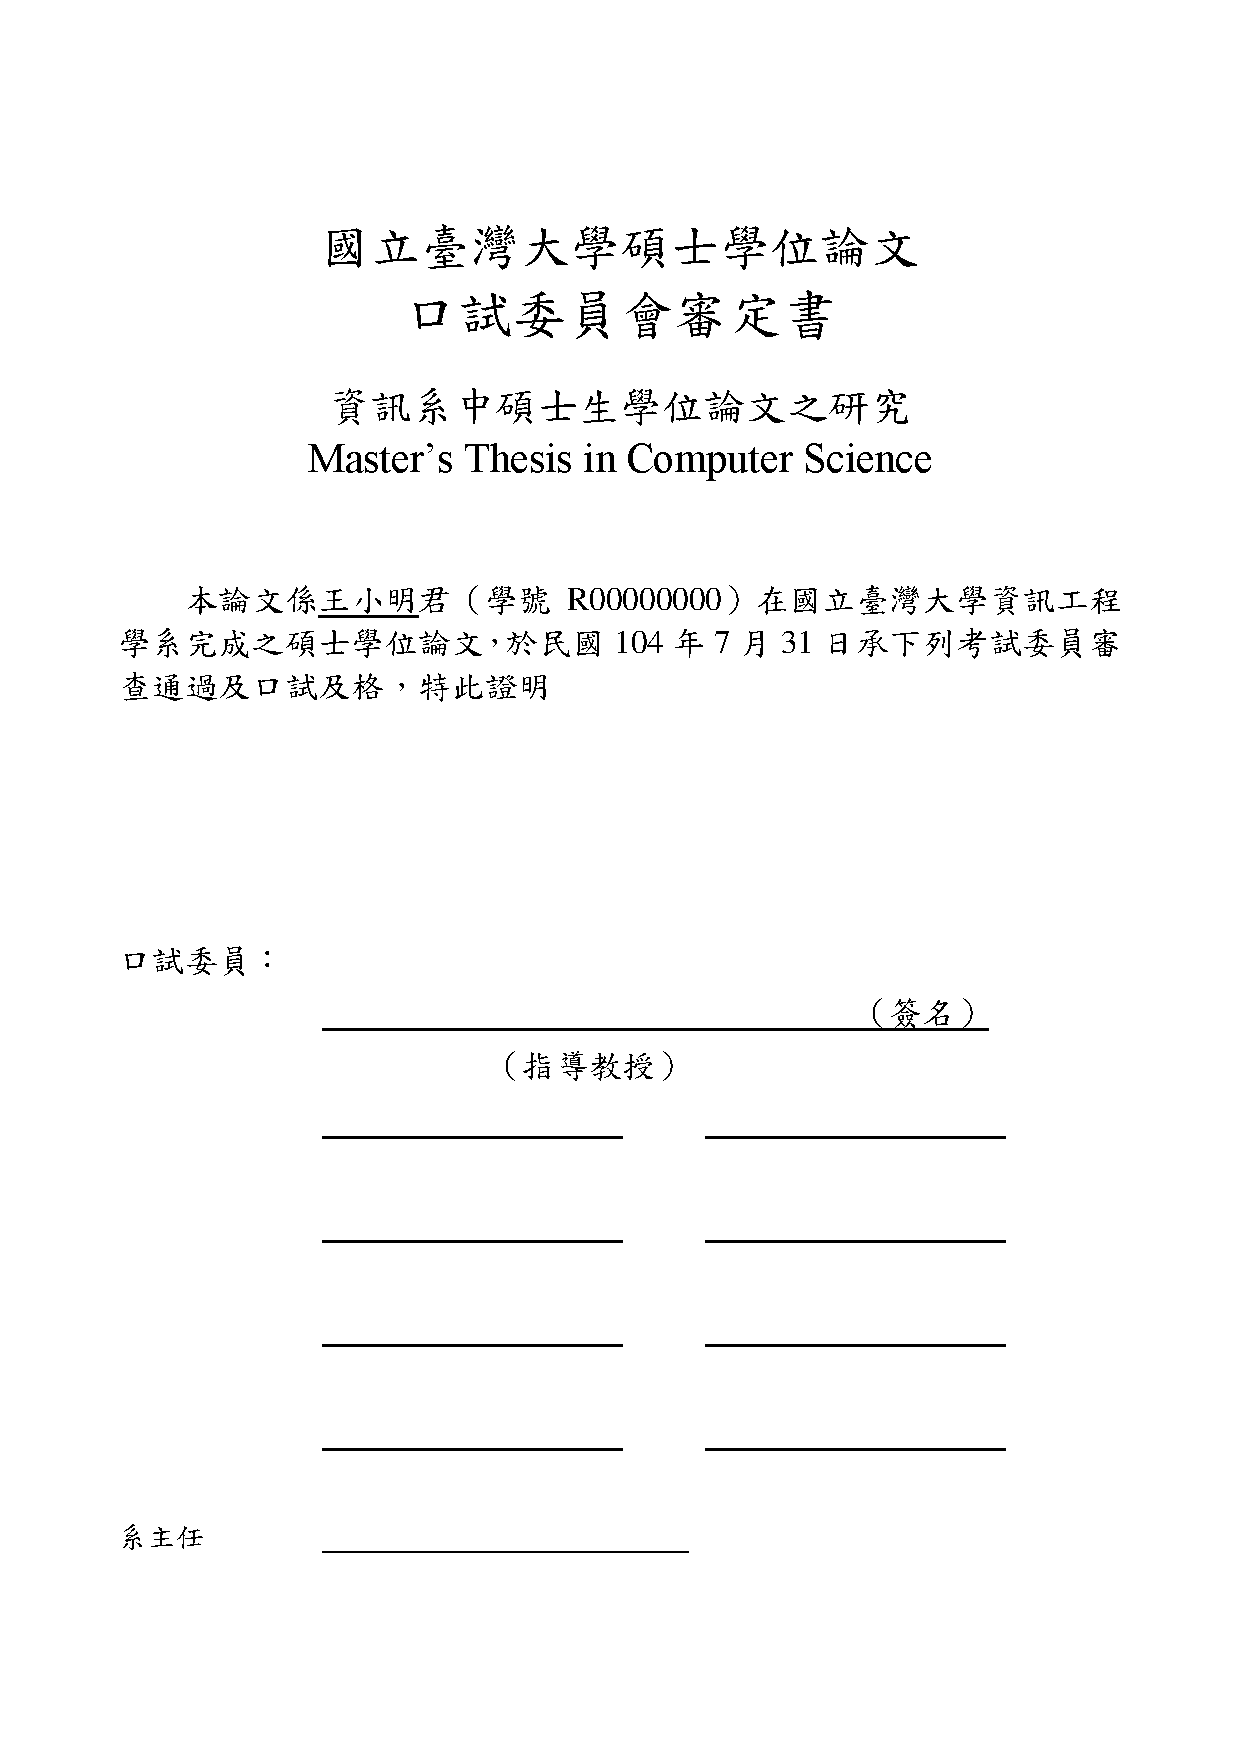
\includepdf[pages={1}]{pdfs/cert.pdf}

\begin{acknowledgementszh}

感謝指導老師莊曜宇教授,提供全方面的資源支持我研究,給予我充份的空間與機會去嘗
試各種新的技術與想法。謝謝蔡孟勳老師提供我諸多研究點子,及參與實驗室合作案們的
機會。謝謝賴亮全老師在生物、統計上的建議。感謝盧子彬老師提供許多研究發表機會,
申請期間寶貴的建議,改變了我研究生涯。感謝在北京微軟的張益肇博士與許燕老師,你
們開拓了我的研究視野。謝謝張博士教導了我大尺度的領域發展觀察、許老師在北京生活
與學習無時的照顧。我經常懷念夥伴們寫程式時的歌唱、一周一百小時的研究時光。

謝謝學長姐們平日在實驗室的照顧。謝謝建樂學長從大學專題生引領我 miRNA 定序分析
起,到指導我的網站開發與碩論回饋;謝謝嘉珊學姐擔任生物問題的求救對象;謝謝鈺喬
學長雙方面的指導以及臉書上的加油打氣。謝謝承桓學長對伺服器們的維護,讓分析都能
順利完成。也謝謝翔瀚、恆元、勁廷、偉安、沂芳、家郁、耀瑋不論是分析、研究、申請
還是日常的交流與抒壓。 也感謝社群朋友們技術分享與生涯規劃的諸多啟發,以及讓我犯
錯冒險的機會。感謝 R 社群的 Wush、c3h3、chiawei、yen 引領我進入開源的大家庭。謝
謝 Python 社群的 yyc、TP、Tim、Andy、Michelle、Keith。沒有你們,我沒有今日的技
術、能力、想法、以及工程師的世界。也謝謝家人、攝影社朋友、高中同學們一路上的支
持。

加入實驗室團隊轉瞬已四年時光,再次感謝所有指導老師、所有實驗室同仁以及朋友的幫
忙。

\hfill 王亮博\quad2016 年 7 月
\end{acknowledgementszh}

%\begin{acknowledgementsen}
%\end{acknowledgementsen}
% vim: set tw=79:

\begin{abstractzh}
随著次世代定序技術的問世,它已經成為基因體研究中最重要的資料來源之一。與傳統的
方法比較,次世代定序能在可行的時間與預算內,提供高通量的序列以及定量生物體活動
的能力。然而,在獲取生物上有意義的結果之前,完成一個次世代定序的分析需要一系列
命令列下運作工具的參與,以及龐大的計算資源,給予生物學家以及臨床人員很高的分析
進入門檻,他們甚而無法解讀自己的序結資料。因此本研究提出了一個線上分析次世代定
序平台,BioCloud,它得以自動化常見的定序分析流程,並且根據分析結果產生總覽報
表。進一步,使用者能設計自訂的分析流程並擴充現有的流程實作來支援更多種類的定序
與分析方法。藉由在 BioCloud 上分析次世代定序,研究者能以更互動式與方便的方式來
了解他們的資料,並且讓整個分析更容易地重現。

\vspace{1.5em}\noindent
關鍵字:次世代定序、線上分析平台
\end{abstractzh}

\begin{abstracten}

With the advent of next-generation sequencing (NGS), it has become one of the
most important data sources in genome-wide study. Compared with traditional
methods, NGS provides high throughput sequencing reads and ability to quantify
expression of biological activities in feasible range of time and budget.
However, before obtaining biologically meaningful results, a NGS data analysis
involves series of command-line tools to process and requires extensive
computation resources, which imposes a high barrier for biologists and
clinicians to enter NGS analysis and even interpret their own data. Therefore,
in this study, an online NGS analysis platform, BioCloud, is proposed to
automate common analysis pipelines and generate summary report based on the
analysis results. Furthermore, users can design their custom analysis pipelines
and extends the existed implementation to support a wider set of NGS sequencing
types and analysis methods. By conducting NGS analyses on BioCloud, researchers
can understand their data in a more interactive and convenient way and the
analyses results can be easily reproducible.

\vspace{2em}\noindent
Keywords: Next-generation sequencing, online analysis platform
\end{abstracten}

% vim: set textwidth=79 spell:


% Table of Content
\clearpages
\tableofcontents
% List of Figures
\clearpages
\listoffigures
% List of Tables
\clearpages
\listoftables

\mainmatter

% Your thesis goes here
\chapter{Introduction}
\label{c:intro}

\section{Motivation}
\label{s:motivation}

%
% Why we need an online analysis platform
%

As more and more genome-wide studies rely on next-generation sequencing (NGS)
analysis, there is an increasing demand from both researchers and clinicians to
develop systems to orchestrate and interpret NGS data analysis pipelines. NGS
provides high read throughput which can generate total a few gigabases of read
sequences in a typical experiment run. However, before the read sequences yield
biologically meaningful results, they have to undergo many non-trivial steps
including genome alignment, sequence piling up, variant calling, and transcript
expression quantification which requires hours of computation by high-end
processors.

Combining the demand for fast computation speed and large data storage, NGS
analyses are mostly performed on powerful servers remotely using command line
interface. Therefore, the tools involved are often developed without graphical
interface due to maximum computation efficiency and lack of need. This kind of
terminal-based environment imposes a high barrier for especially biologists and
clinicians to enter. Furthermore, output of most analysis tools are shown as
log files or as file formats that are friendly for computers to parse but
cannot be easily interpreted by human without data cleaning and transformation.

As a NGS service core lab, many lab members have identified the burden of
routine NGS data processing and interpretation of results of commonly used
analysis pipelines. If a graphical summary report can be obtained after the
automated execution of analysis pipeline, many biologists and clinicians can
interpret the result themselves without extensive knowledge of how computers
work nor consulting bioinformatic researchers and thus improve the efficiency
of collaboration. On the other hand, for bioinformatic researchers, automated
execution of typical analysis pipelines can release them from routine tasks to
process incoming NGS experiment runs and focus more on innovative discovery and
interpretation of the NGS data itself.

Several analysis platforms have been proposed to help automate NGS analysis
pipeline with user friendly report or result viewer, including commercial
products such as DNAnexues \cite{:dnanexus} and Partek Flow \cite{:partek} and
open source projects such as Galaxy \cite{goecks2010:galaxy} and Genome
Modeling Tools \cite{griffith2015:genome}. However, these tools are either too
complex for biological researchers and clinicians to use, too simple for
researchers to build their own pipeline, or operating at a scale too large for
our lab to adapt. Therefore, the idea of building our own designed NGS online
analysis platform then emerged and became the main goal of my master thesis
study.


\section{Specific Aims}
\label{s:specific-aim}

%
% Propose the analysis platform and report generator
%

In this thesis study, an online platform, BioCloud, and a report generator,
BCReport, have been developed to help researchers automate their NGS analyses
and interpret the result based on the generated summary report. The online
platform builds on an account system to let individuals manage their sequencing
data sources and then design the experiment and sample settings to group their
data sources like their biological experiment set up. The designed experiment
can be used in different analysis pipelines that match the sequencing type of
the data sources, e.g., DNA or RNA sequencing. Each analysis pipeline combines
different tool chains and comes with their corresponding tool parameters for
user to adjust. After an analysis pipeline has been configured, it is submitted
to the job queue of online platform and will execute the underlying tool chains
when the computation resources are available.

As soon as the analysis execution has been completed, the report generator,
BCReport, is called and generates a summary report by parsing the results of
the execution. Report are given in HTML format so BCReport can be seamlessly
integrated into BioCloud and user can view their report via the BioCloud
website. In the report, the output of each tool is collected and parsed as
interactive charts and tables for user to explore the result. One of the
convenient features about the summary report is that results are grouped by
their samples and condition settings so user can compare the result between
different conditions naturally. They can also download the raw result output by
links provided in the report. Reports and results can be easily shared by
providing their URL link. Though the links are publicly accessible via
internet, they can be well protected if user apply different permission rules
for each analysis.



\section{Next-generation sequencing}
\label{s:ngs}

Next-generation sequencing (NGS) is a group of sequencing technologies that
succeeds automated Sanger sequencing which is considered as the first-generation
sequencing, by providing much higher read throughput while shorter read length
that reduces the cost and time to complete genome-wide sequencing study
\cite{metzker2010:sequencing}. Generally speaking, a NGS experiment undergoes
steps of template preparation, sequencing, imaging and data analysis. During
template preparation, DNA samples are broken into fragments of shorter length,
which the desired length varies across different NGS technologies but generally
in the range of few tens to few thousands of nucleotides. Proper adapters and
barcode will be added to these DNA fragments for further manipulation, fixation
on the sequencing chip, and mixed multiple samples in one experiment run. Each
template will then be positioned separately on the sequencing chip by for
example, ligation with adapter in illumina NGS technology. Sequencing is done
by multiple cycles which read out one base at a time using deoxyribonucleotide
triphosphates (dNTPs) with four or two fluorescent chemical labels and
reversible terminator. Reading base detection in a sequencing cycle is done by
image capturing the fluorescent emission of all templates on chip. Sequencing
and imaging steps enables NGS determine the sequencing millions of DNA
fragments in parallel.

Next-generation sequencing has been playing an important role in current
genomic researches. In the last decade, next-generation sequencing has become
the \textit{de facto} way to understand genome \cite{vandijk2014:ten} including
quantification of transcriptome expression \cite{wang2009:rnaseq}, variant
calling and genotype inference \cite{nielsen2011:genotype}. The ability to
determine novel sequence reads opens the door for \textit{de novo}
transcriptome and genome assembly. Comparing to the renowned Human Genome
Project \cite{lander2001:initial}, finishing a new organism assembly now
requires significantly shorter time and lower budget and makes study of
non-model organisms becoming feasible. As the sequencing cost for a whole human
genome passing below USD 1,000, we can expect a wider application of NGS and
more and more fields adopt this technology.

% single-cell sequencing
New single-cell sequencing technology, often viewed as the third generation
sequencing, has enabled the genomic research down to the cellular level in the
past few years \cite{gawad2016:singlecell}. New insights may be found by
applying single-cell sequencing to heterogeneous samples, for example, studying
somatic mutations in tumor samples and analyzing individual genomes in
metagenomics. Although the sequencing data from single-cell sequencing may have
different properties with that from NGS, including statistical distribution and
sequencing error model, the overall workflow and file format for data storage
shares a lot in common. Therefore the currently developed analysis platform can
still analyze data from future sequencing technologies without large
modification.



\section{Genome reference}
\label{s:genome-ref}

Once a NGS experiment is complete, the sequence reads are merely sequences of
DNA fragments and lack biological meaning. However, since fragments are often
overlap with each other, one can concatenate fragments into longer sequences
called scaffolds. Multiple scaffolds can later construct chromosomes and hence
complete a whole genome sequencing. The whole process of joining reads into
scaffolds and chromosomes is referred to as genome assembly. The counterpart
for RNA sequencing and cDNA fragments is referred to as transcriptome assembly.
If such sequence assembly is done on a novel organism, the assembly is called
a \textit{de novo} assembly.

However, \textit{de novo} assembly requires high sequencing coverage and takes
substantial computing resources, which is not feasible for normal applications.
Also, it is hard to comparing the results based on genome from different
studies if people rely on their own distinct genome assembly. Many genomic
studies requires integration of multiple annotations including gene, transcript,
and variant formation, thus having sufficient number of sequencing runs, a
consensus of genome assembly forms the genome reference. A genome reference
needs not to be the exact sequence of a specimen but represents the most common
sequence of the given genomic region.

Once a genome reference is released, different types of annotations, e.g.,
different gene databases, are aligned to the new genome reference. These
annotations can be browsed by the given chromosomal location via genome
browser. Normal applications now only needs to align to the genome reference,
which not only save both time and cost, but also are able to access to many
other annotations. Thus for model organisms like human and mouse, analyses
generally relies on certain version of genome reference.

% time and cost
% hard to compare other result
% annotations

NGS currently still has its limitations to cover full genome in a sequence run.
There are still regions and special sequencing patterns which are hard to
sequence, including reads with short repeat and high GC\% content; regions in
centromeres and telomeres. Even if they can be sequenced correctly, their
repetitive sequences make it hard to figure out the right assembly. Therefore,
even for the mature genome projects like human genome project, the genome
sequence is continually updated. The latest human genome reference GRCh38.p7
was released in March 2016, and it still contains 805 scaffolds with 349 gaps
\cite{:grch38p7}, whereas the first version released in 2001 contains around
150,000 gaps \cite{2010:e-pluribus-unum}.

% allelic diversity -- alternative loci
% patch

It should be noted that there are two types of genome reference updates: major
and minor updates. Major updates, e.g., from hg19 to GRCh38, breaks the
chromosomal location compatibility, whose genomic coordinates of primary
assemblies, e.g., major chromosomes and plasmids, will change. One could use
tools such as liftOver to handle the coordination conversion. On the contrary,
minor updates, e.g., from GRCh38 to GRCh38.p1, don't introduce backward
breakage on primary assemblies, but release the updates as patches and
alternative loci. Patches fix the sequencing errors or fill in the gap between
scaffolds of primary assembly, which will be displayed along their
corresponding genomic regions and overwrites the primary assembly in the next
major release. Alternative loci appear in when some regions have high allelic
diversity so one common sequence cannot well represent the specified gnomic
region. For example, major histocompatibility complex (MHC) region on
chromosome 6 has 7 alternative representations.


%
% Explain about the general NGS analysis workflow
%

\section{General NGS analysis workflow}

Except for \textit{de novo} assembly, general NGS analysis involves the
following analysis steps: sequencing quality check, genome alignment,
annotation, and statistical inference. During sequencing, the sequencer records
each read base with a Phred quality score $q$, where the probability of the
base being erroneously sequenced $P_q$ is $P_q = 10^{\frac{-q}{10}}$. A read
base with quality lower than 30 implies the probability of sequencing error at
this base is higher than 0.1\%. How quality is measured depends on the
sequencing technology. For example, the quality score is computed based on the
fluorescent intensity on Illumina platforms. Quality of all sequence reads will
be first checked to determine if the experiment run performed as expected.
Reads with low quality can be filtered or partially trimmed during this stage.

% genome alignment
Then sequence reads are aligned to the genome using certain version of genome
reference. Though the generated sequence reads are shorter, they are long
enough to determine their genomic location. Aligned reads may have mismatched
sequences with genome reference and the all alignment information will be
stored in the alignment result file, usually in the format of BAM or SAM files.
Alignment methods of RNA and DNA sequencing are different, since RNA-Seq the
sequences are the product of splicing event and will map to multiple distinct
exon regions during alignment. After sequences have been aligned to the genome,
user can annotate the reads about the gene information it locates, whether the
variant is a common SNP. The annotation in use will depend on the type of
sequencing and intended application, as long as annotation and the sample
alignment share the same version of genome reference. With proper annotation,
statistical inference and modeling help researcher answer questions like how a
gene or transcript is expressed, whether a genomic location has mutation, or a
genomic region has copy number gain or loss.


% \section{RNA and DNA sequencing application}
% RNA-Seq
% - differential expression
% - novel isoform/transcript discovery
% - de novo transcriptome assembly
%
% DNA-Seq
% - SNV variant calling
% - germline mutation
% - somatic mutation
% - CNV
% - de novo assembly


% vim: set textwidth=79 spell:

\chapter{Related Works}
\label{c:related-work}

In the following, BioCloud is compared with currently available and popular
frameworks, tools and platforms for either NGS analysis pipeline execution or
result report generation. Overall, commercial products such as DNAnexus and
Partek Flow provide more comprehensive functionalities and support than open
source projects and tools. Comparison between a larger sets of related works
can be found in \citeauthor{leipzig2016:review}'s study
\cite{leipzig2016:review}.


\section{Commercial online analysis platforms}

DNAnexus \cite{:dnanexus} is an commercial cloud-based sequencing data analysis
platform, which is undoubtedly the most feature-rich platform currently
available. The role DNAnexus plays in a typical sequencing-driven study is
illustrated in Figure~\ref{fig:dnanexus-workflow}. It covers sequencing samples
management, online analysis pipeline execution, and a result view integrated
with its custom crafted genome browser. All of its functionalities are designed
to be user friendly and does require little understanding of programming and
how to mangle with multiple sequencing formats. However, due to its by-design
simplicity, user can not easily customize their own pipeline to adopt new
published tools or update the tool version in use. On top of that, the usage of
clinical data may be subjected to different law restrictions in different
countries. Using service and cloud sever hosted and managed by a United States
company may not meet the law restrictions in Taiwan and raises extra concern
and private issues for hosting data with patient and clinical information.

\begin{figure}[!htbp]
\centering
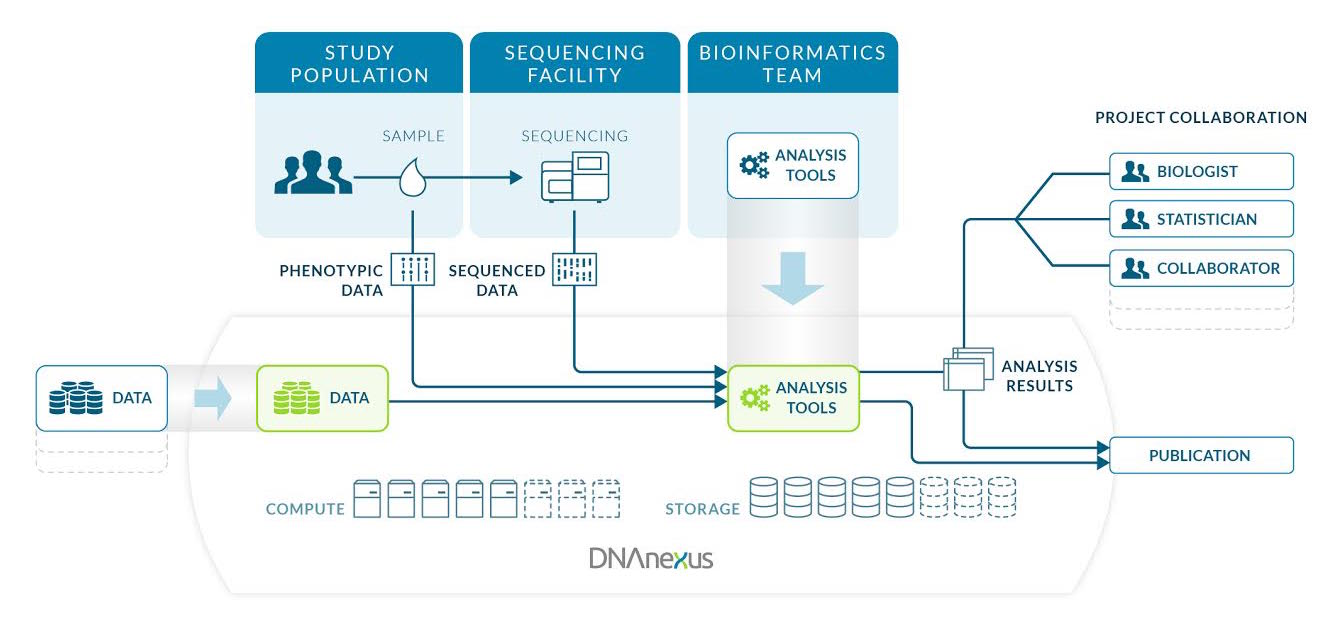
\includegraphics[width=\textwidth]{images/dnanexus_workflow}
\caption[DNAnexus workflow]{
    The role of DNAnexus in a typical sequencing-driven study. User or the
    sequencing facility can upload raw sequencing samples to the DNAnexus and
    complete the rest of the analysis on its platform. The workflow is obtained
    from \href
    {https://www.dnanexus.com/images/diagram/img-platform-genome.jpg}
    {DNAnexus's official website}.
}
\label{fig:dnanexus-workflow}
\end{figure}


Another commercial product, Partek Flow \cite{:partek}, focus more oriented to
bioinformatic researchers by offering custom pipeline design and online
analysis pipeline execution. An example of the custom pipeline design on Partek
Flow is shown in Figure~\ref{fig:partek-flow-pipeline}. User can drag and drop
different function blocks from its tool panel and connect them as a pipeline,
which is very flexible for researchers to explore different combinations of
tools. For different function blocks they can append with different type of
reports or quality assessment. The whole system can be hosted on one's own
server. Due to its flexibility of pipeline design, however, Partek Flow user
should be familiar with all analysis tools involved before conducting new
analysis. Though viewed convenient by bioinformatic researchers, it has a
relatively complex interface to design and execute analysis pipelines.

% TODO: update with our lab's screenshot
\begin{figure}[!htbp]
\centering
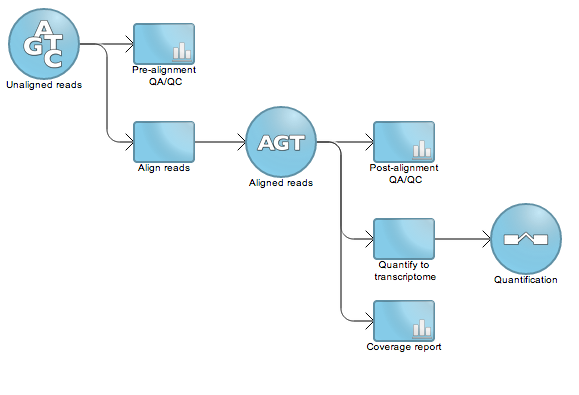
\includegraphics[width=0.7\textwidth]{images/partek_flow_pipeline}
\caption[Example of custom pipeline design on Partek Flow]{
    Example of custom RNA-Seq analysis pipeline design on Partek Flow. It first
    use gnome aligner STAR to align the sequencing, and then use Cufflinks
    quantify the transcript expression. Pre-alignment and post-alignment
    quality check are added. An alignment coverage report is added after
    alignment. The custom pipeline is obtained from
    \href{http://www.partek.com/star-align-and-quantify}{Partek Flow's official site}.
}
\label{fig:partek-flow-pipeline}
\end{figure}




\section{Open sourced online analysis platform}

The Galaxy project \cite{goecks2010:galaxy} is the most widely used general
purpose bioinformatic analysis platform, which aims for reproducible research
in computational biology. Like commercial platforms previously mentioned,
Galaxy can let user upload and manage their own data sources, execute tools
remotely, and convert the execution history into reproducible workflow via its
flexible workflow editor. Galaxy can be deployed on one's own cloud or server,
while they also maintain a list of public Galaxy servers with commonly used
toolboxes to let anyone to try on freely. Support for NGS data analysis has
reached a relatively mature state where most common tools are available and can
be accessed on their public servers. Figure~\ref{fig:galaxy-workflow} shows how
a typical RNA-Seq analysis workflow called Tuxedo looks like in Galaxy's
workflow editor, which best demonstrates the powerfulness and flexibility the
editor provides. However, it is more specifically designed for bioinformatic
researchers than Partek Flow. Also it has been developed for years, some of the
Galaxy dependencies make its source code obscure for normal Python developers,
which they often craft their own tool chains without adopting language agnostic
standards. A pile of specially developed tool chains make the Galaxy plugin
development more difficult then it seems at first. It may also lead to security
issues since most of their own developed web tools have not been publicly
battle tested, whereas standard Python web frameworks and tools like Flask and
Django have been audited and publicly tested by worldwide companies for years.

\begin{figure}[!htbp]
\centering
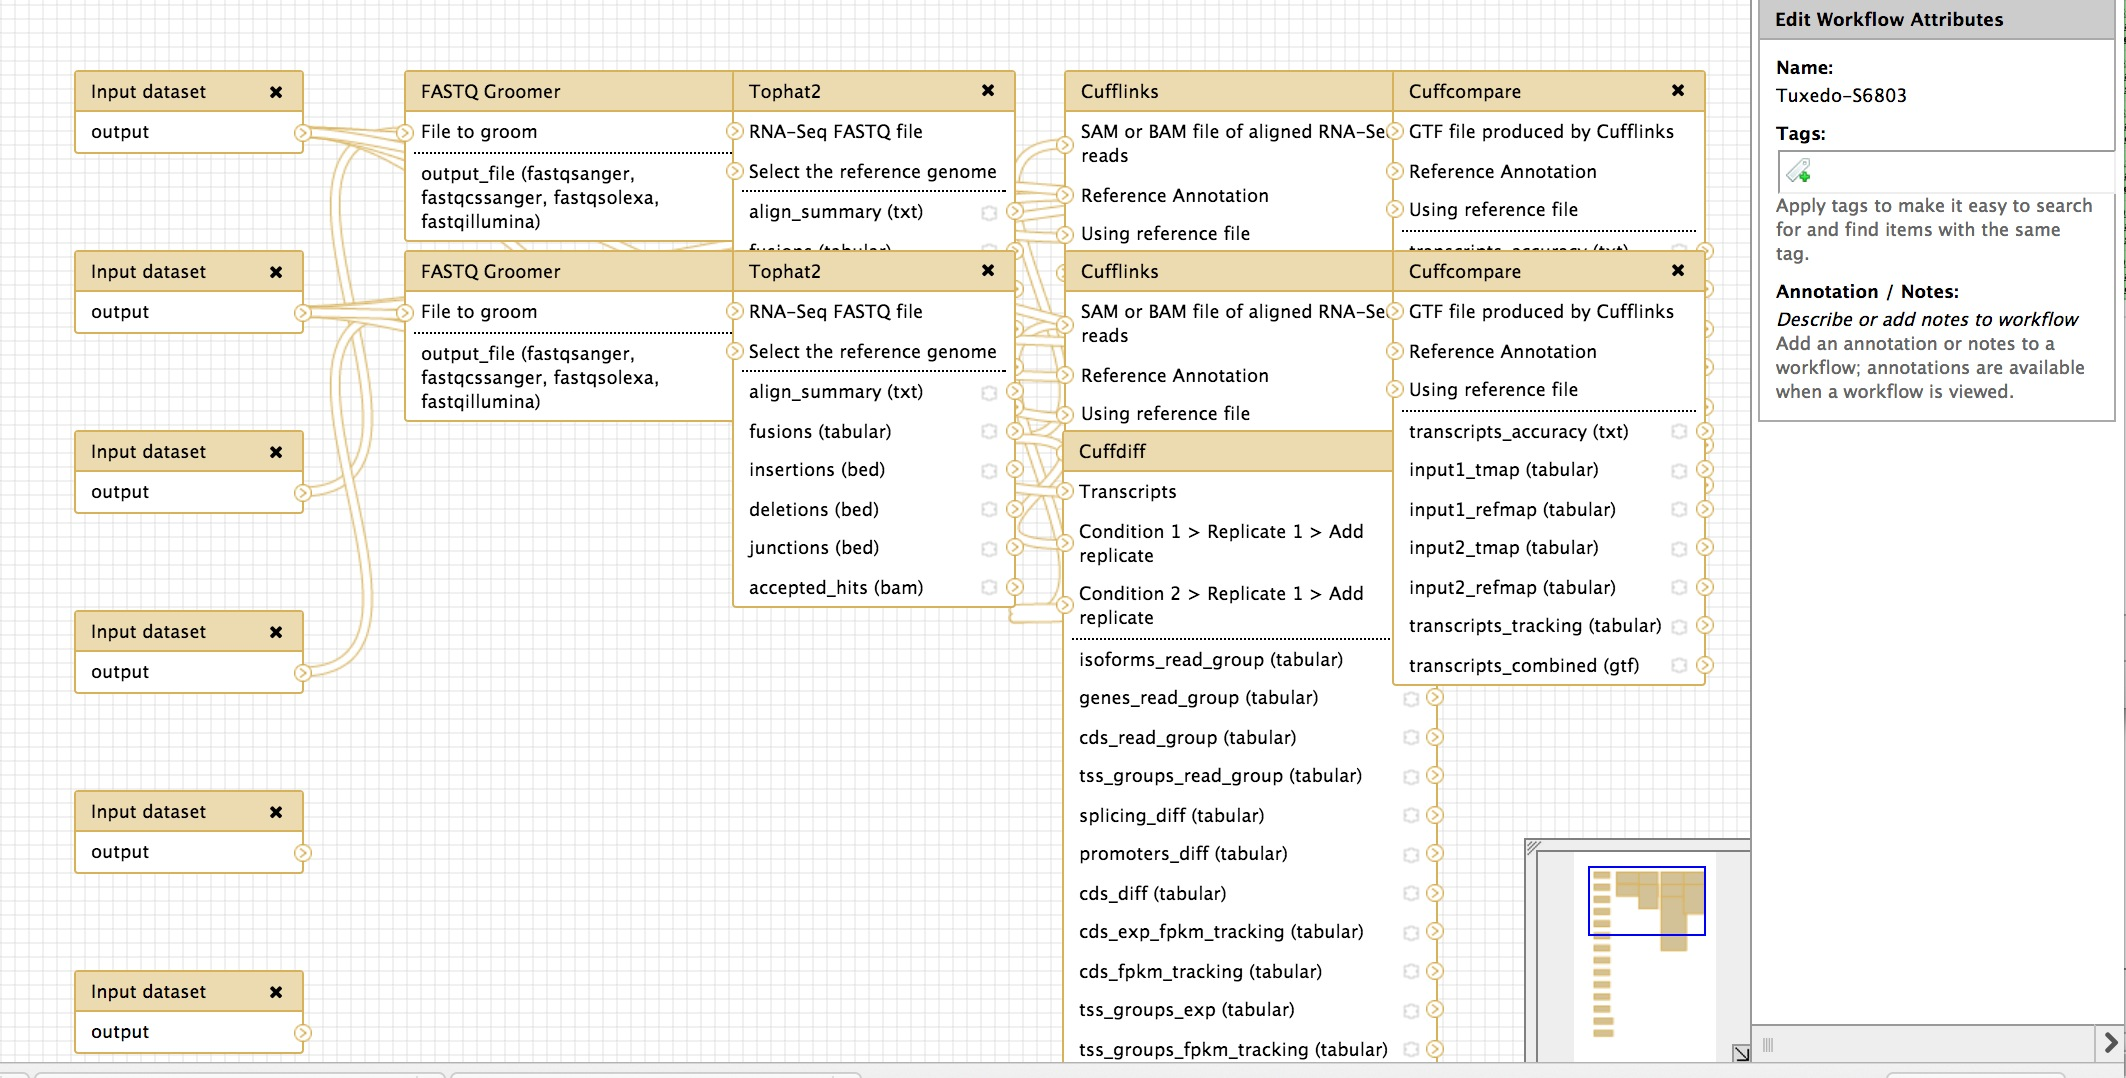
\includegraphics[width=1\textwidth]{images/galaxy_workflow}
\caption[Example of custom workflow on Galaxy]{
    Example of custom workflow on Galaxy implementing the Tuxedo RNA-Seq
    analysis workflow. This RNA-Seq workflow uses Tophat2 as genome aligner and
    Cufflinks for transcript expression inference. The shown custom workflow is
    developed and obtained from
        \href{http://genomeintelligence.org/?p=561}
        {Genome Intelligene website}
    made by Dr. Cynthia Gibas.
}
\label{fig:galaxy-workflow}
\end{figure}




Another sequencing analysis platform, Genome Modeling System
\cite{griffith2015:genome}, is used in The Genome Institute of Washington
University and has process hundreds of terabytes of sequencing data with
predefined hundreds of bioinformatic tool profiles. It resembles Galaxy in the
flexibility of developing custom workflow, while focusing solely on processing
sequencing data. Using the terminology of Genome Modeling System, sequencing
sources are subjects, and user can define multiple genome model on the same set
of subject. Genome model is defined by connections of tool profiles. Tool of
different versions have different profiles to ensure the result of genome model
can be strictly reproducible using pinned version of tools. However, like
Galaxy, it has a relatively complex design of pipeline design and does not suit
for biological researchers and clinicians.


\section{Pipeline execution tools}
\label{s:pipeline-execution-tool}

Though some of the works are not a full-fledged online analysis platform, they
focus on the automated analysis pipeline design, including bcbio-nextgen
\cite{:bcbionextgen,guimera2012:bcbionextgen} and Snakemake
\cite{koster2012:snakemakea}, whose architecture designs either share common
traits with BioCloud or inspire some features of BioCloud.

In bcbio-nextgen \cite{:bcbionextgen,guimera2012:bcbionextgen}, user can adopt
existed or design custom analysis type, and then specify the input samples,
genome reference, and other necessary parameters through a pipeline
configuration file in YAML format, which is human readable and simple to write
from scratch in plain text. An configuration example of RNA-Seq analysis is
shown in Listing~\ref{lst:bcbio-nextgen-config}, whose structure and syntax
share plenty of common with BioCloud's analysis configuration file.
Bcbio-nextgen by default ships with predefined of DNA-Seq, RNA-Seq, small
RNA-Seq, and CHIP-Seq pipelines so real analysis can be performed with little
effort. The pipeline execution can utilize multi-core processors and even scale
across multiple machines through IPython Parallel framework
\cite{:ipython-parallel}. Scripts to deploy on Amazon Web Service (AWS) are
available so user can scale up the number of AWS computing instances
dynamically when needed. Bcbio-nextgen is also gradually adding support of
Common Workflow Language \cite{amstutz2016:common}, which is a on-going
workflow specification standard proposed by multiple analysis platform vendors.
The integration of IPython Parallel framework and AWS cloud infrastructure
makes bcbio-nextgen a competitive tools to perform large scale and parallel
pipeline analysis.

\begin{lstlisting}[
    caption={
        Example of bcbio-nextgen pipeline configuration to run Tophat2 genome
        alignment. The configuration is obtained from the
        \href{https://bcbio-nextgen.readthedocs.io/}
        {official tutorial of bcbio-nextgen}.
    },
    label={lst:bcbio-nextgen-config},
    language={},
]
fc_date: '070113'
fc_name: control_experiment
upload:
    dir: final
details:
    - files: [
          /full/path/to/control_1.fastq,
          /full/path/to/control_2.fastq
      ]
      description: 'Control_rep1'
      genome_build: GRCh37
      analysis: RNA-seq
      algorithm:
           aligner: tophat2
           quality_format: Standard
           trim_reads: read_through
           adapters: [truseq, polya]
           strandedness: unstranded
\end{lstlisting}

Snakemake \cite{koster2012:snakemakea} is a low-level pipeline execution tool
which is inspired by source code build automation tool Make \cite{:gnu-make}
and its rule file format Makefile. User constructs a Snakemake pipeline by
writing a series of rules which each rule corresponds to commands of a tool.
Each rule also defines its input and output file patterns, which Snakemake will
use them to construct the execution dependencies between rules as a directed
acyclic graph (DAG). Listing~\ref{lst:snakemake-rule} shows an example of
writing Snakemake rule to run BWA MEM genome alignment. Like Makefile, the
variable \texttt{\{sample\}} specified in the input FASTQ files will be auto
expanded to all files matching the given pattern, that is, all files with
suffix \texttt{.fastq} under the folder \texttt{data/samples/}. Before
execution, these rules are first evaluated and expanded to all matched files to
build the DAG dependencies, shown in Figure~\ref{fig:snakemake-dag}. Snakemake
will detect outdated output files by comparing creation timestamp with input
files. Only outdated outputs will be re-executed, which reduces the total
execution time. Other parameters of the Snakemake rule can further control the
resources a job can use, e.g., number of threads and read-only files to prevent
output files from being rewritten.

\begin{lstlisting}[
    caption={
        Example of Snakemake rule to run BWA MEM genome alignment. The rule is
        obtained from the
        \href{http://snakemake.bitbucket.org/snakemake-tutorial.html}
            {official tutorial of Snakemake}.
    },
    label={lst:snakemake-rule},
    language={},
]
rule bwa_map:
    input:
        "data/genome.fa",
        "data/samples/{sample}.fastq"
    output:
        "mapped_reads/{sample}.bam"
    shell:
        "bwa mem {input} | samtools view -Sb - > {output}"
\end{lstlisting}

\begin{figure}[!htbp]
\centering
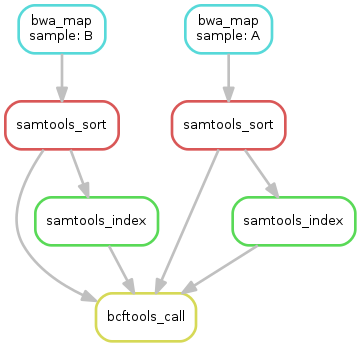
\includegraphics[width=0.5\textwidth]{images/snakemake_dag}
\caption[Example of DAG job dependencies of a Snakemake workflow]{
    Example of DAG job dependencies of a Snakemake workflow that first aligns
    sequence reads to genome using BWA MEM, sorts and indexes the aligned BAM
    file, and finally calls variants using bcftools. Two samples A and B are
    used, and Snakemake can correctly understand the input and output
    dependencies for each job through file expansion and collection rule. The
    workflow is obtained from
    \href{http://snakemake.bitbucket.org/snakemake-tutorial.html}
    {the official tutorial of Snakemake}.
}
\label{fig:snakemake-dag}
\end{figure}




Though Snakemake may not be directly used by biological researchers and
clinicians, integrating it into a cloud platform may not be as trivial as it
seems. Monitoring the Snakemake execution process can be complicated since it
treats individual inputs as separate jobs. One could either show the detailed
execution progress or trying to deep integrate with Snakemake to collect all
the job details and organize them externally. The latter deep integration can
be easily broken if Snakemake changes its internal structure.

Two pipeline execution tools mentioned above can be used as the way Biocloud
run analysis pipelines. However, due to time constraint and development
complexity a developer can manage, BioCloud rolls out its only basic pipeline
execution method with stage monitoring. There are possibilities for BioCloud to
leverage these pipeline execution tools in future and such integrations are
discussed in Chapter \ref{c:discussion}.


\section{Analysis report generation}
\label{analysis-report-generation}

An analysis report helps summarize the result of a sequencing analysis pipeline
across different samples or even different conditions in the experiment design.
Without getting into details, summary report collects the most important
statistics and results of each tools, which is suitable to provide researchers
with little sequencing experience a basic understanding the condition of one's
sequencing results.

Aside from commercial products which more or less provide a summary report,
some open sourced works also focus on the summarization of the sequencing
analysis. MultiQC \cite{ewels2016:multiqc} is a quality assessment tool for
sequencing data. After its first release in Nov 2015 it has been gaining
popularity. At the time of writing, both bcbio-nextgen and Galaxy can integrate
with MultiQC report. An example of the MultiQC report is shown in
Figure~\ref{fig:multiqc-report}, which is a single page HTML report. The first
general information table collects important statistics of each sample produced
by each tools, which user can select which of them should be displayed by
tweaking the column visibility. Following the general information, the report
shows interactive figures which user can zoom in and out, filter unwanted
samples, and export current figure state as static JPEG or PNG picture format.

However, since MultiQC focuses on quality assessment, it cannot parse the end
results of typical sequencing analysis. MultiQC treats samples independently,
so user cannot group samples of same conditions or compare samples grouped by
their conditions. For example, it cannot display the differentially expressed
genes and genomic variants called in all samples of the same condition. Also,
due to its single page web structure, showing figures of too many stages will
impact the viewing experience due to low rendering frame rate. Though MultiQC
does provide innovative ways to display sequencing results, BioCloud cannot
directly integrate MultiQC and need to develop its own way displaying figures
considering sample grouping.

\begin{figure}[p]
\centering
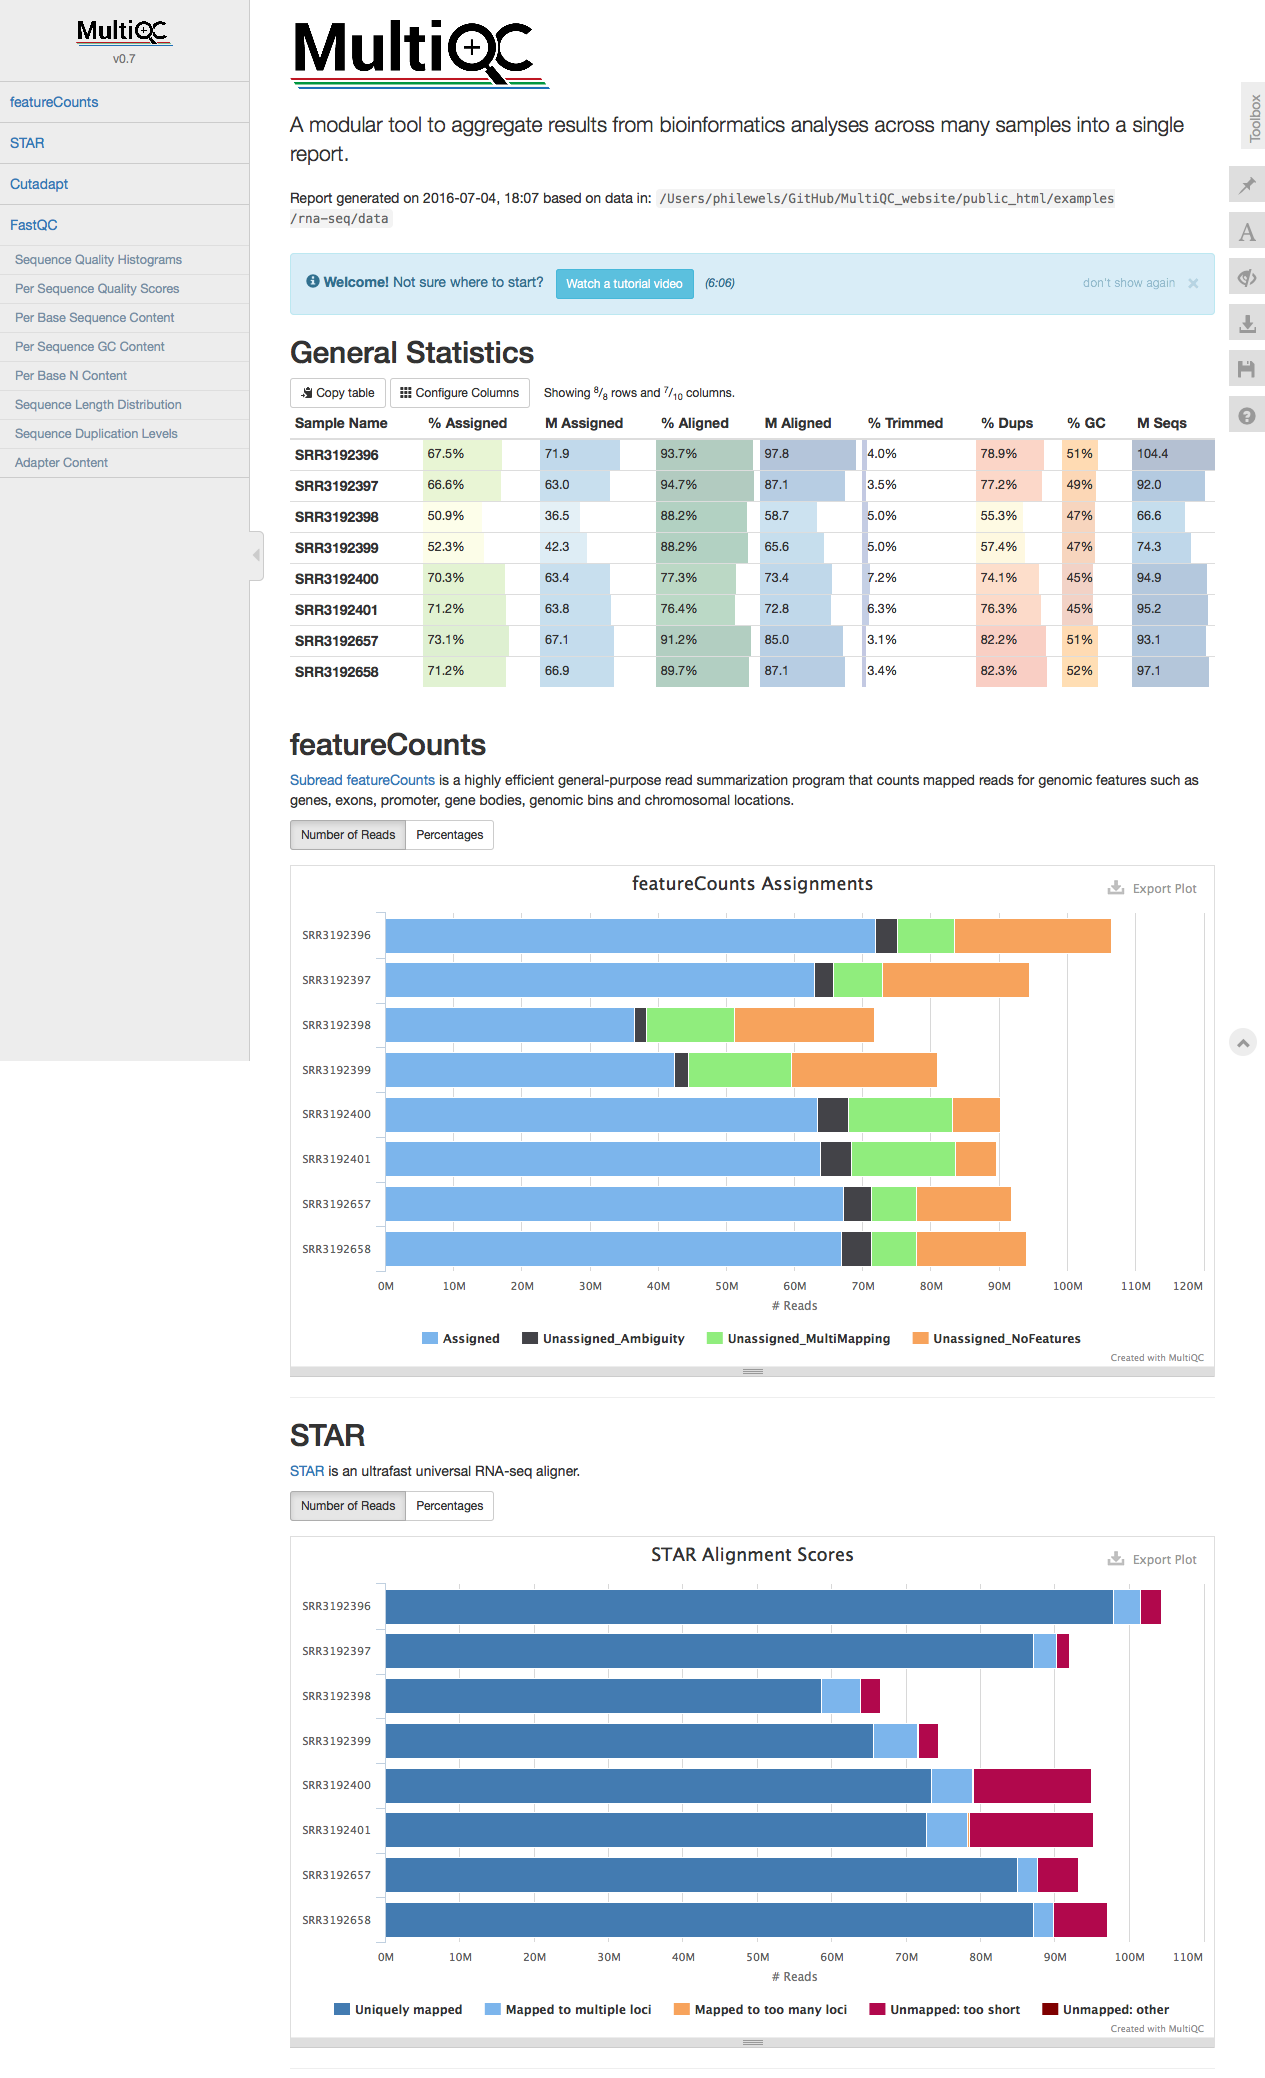
\includegraphics[width=0.9\textwidth]{images/multiqc_report}
\caption[Example MultiQC report]{
    Example MulitQC report for RNA-Seq analysis.
}
\label{fig:multiqc-report}
\end{figure}




% vim: set textwidth=79:

\chapter{Methods}
\label{c:method}

In the following sections, first a number of typical RNA-Seq and DNA-Seq
pipelines that BioCloud supports are defined and explained. Then the design of
BioCloud is explained by breaking down into two main parts: the website and the
report generator. For the website, the components including account
registration, data sources management, experiment design, and pipeline
execution are described and their roles are illustrated in the website overview
workflow. For the report generator, the workflow is shown to demonstrate how
outputs of each tool is extracted, parsed, and rendered into pre-defined
web-based report templates.



\section{RNA-Seq pipelines}
\label{s:rnaseq-pipeline}

The RNA-Seq analysis pipelines that BioCloud supports are summarized in
Figure~\ref{fig:rnaseq-pipeline}, where some of the tools are shared for
different pipelines. The goal of RNA-Seq analysis is to infer differential
expression of gene or transcripts across different conditions. Based on
different assumptions of the distribution of gene and transcript expression,
three different methods are used: Cufflinks, DESeq2, and kallisto, which yield
FPKM based, count-based, and abundance-based expression value respectively.

\begin{figure}[!htbp]
\centering
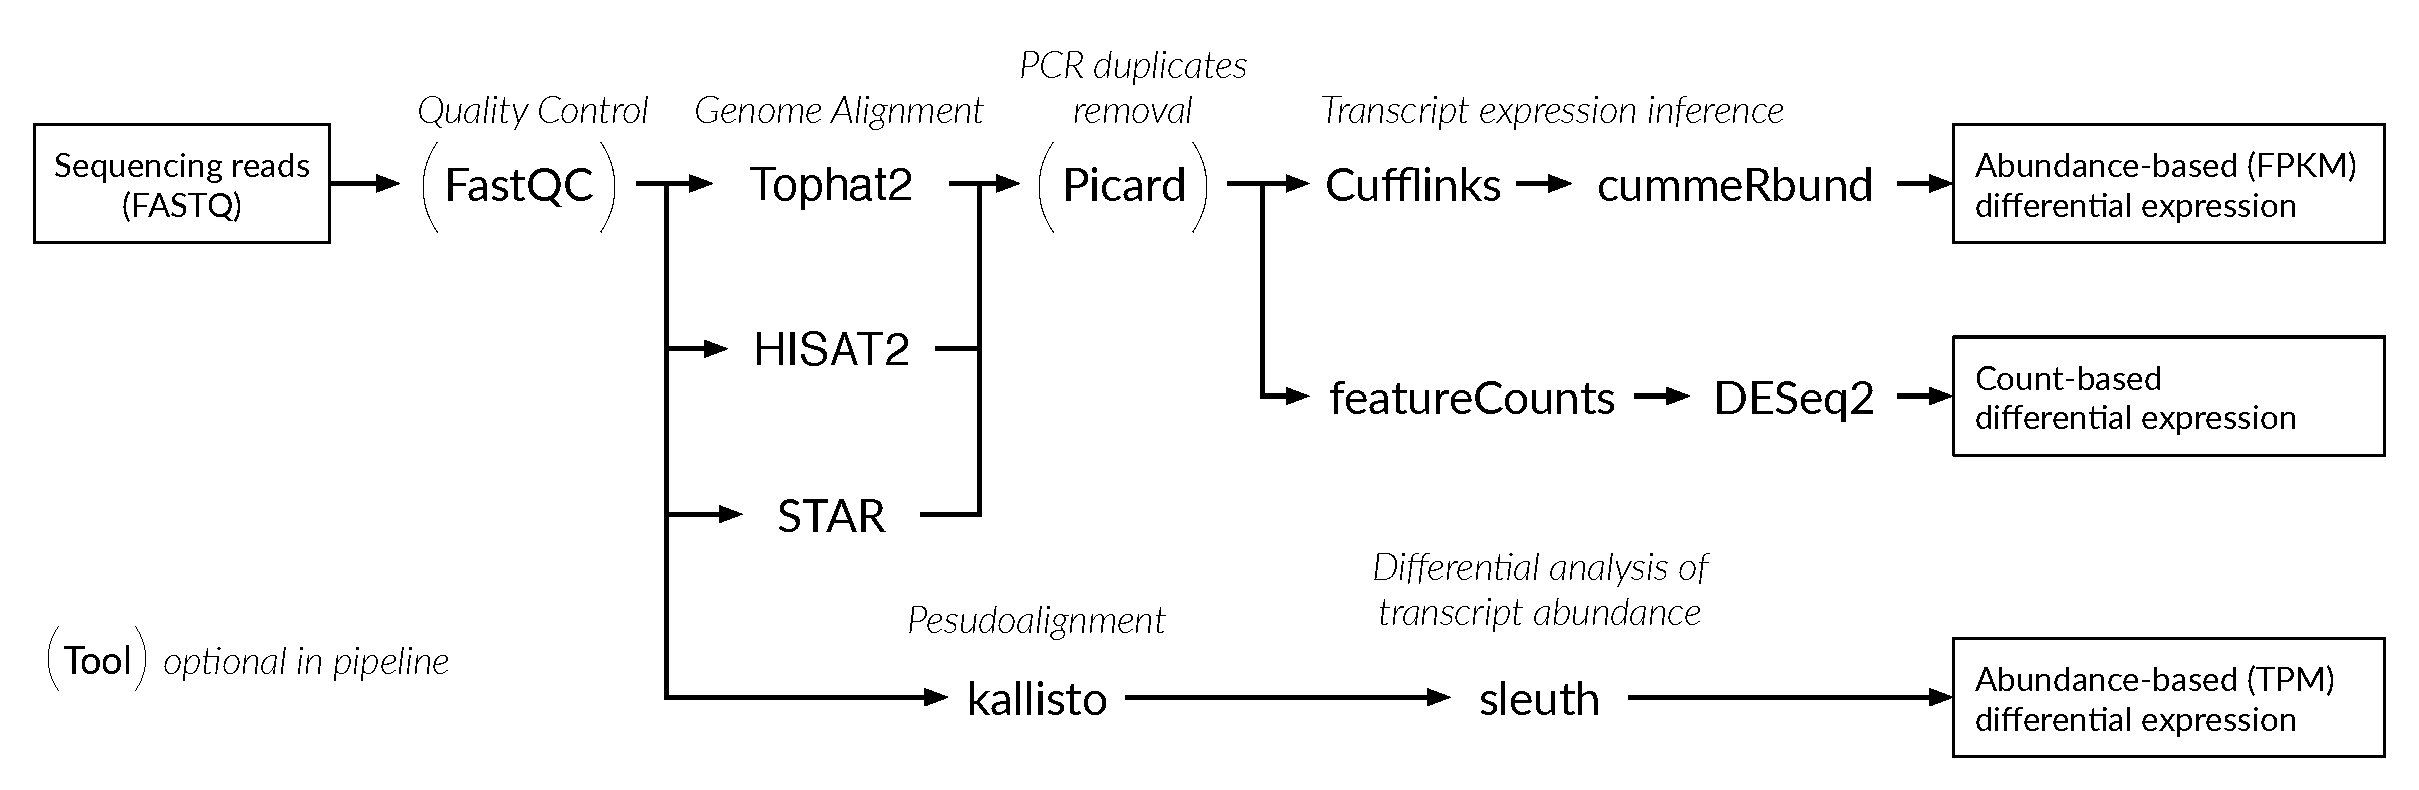
\includegraphics[width=\textwidth]{images/rnaseq_pipelines}
\caption[RNA-Seq analysis pipelines]{RNA-Seq analysis pipelines supported by BioCloud.}
\label{fig:rnaseq-pipeline}
\end{figure}


Cufflinks \cite{trapnell2010:transcript} and its differential analysis method
Cuffdiff \cite{trapnell2013:differential} are best used for gene expression
considering its isoforms, e.g., differential expression on transcript-level.
The output of Cuffdiff can be further visualized using R package cummeRbund
\cite{:cummerbund} from the same development team of Cufflinks. The unit of
expression Cufflinks uses is reads per kilobase of exon per million reads
mapped (FPKM). For DESeq2 \cite{love2014:moderated}, its model analyzes
expression change on gene level using read counts, which cannot be applied to
transcript level analysis. The unit of expression DESeq2 uses is normalized
read counts. The read counts are computed by featureCounts
\cite{liao2014:featurecounts}. Another popular alternative for computing read
counts is HTSeq \cite{anders2015:htseqa}. HTSeq generally acts the same as
featureCoutns while having slower processing speed so it is not used in
BioCloud.

Both Cufflinks and DESeq2 require genomic location of reads so their analysis
is prepended by the genome alignment step. Three aligners are supported:
Tophat2 \cite{kim2013:tophat2}, HISAT2 \cite{kim2015:hisat}, and STAR
\cite{dobin2013:star}. Though the underlying alignment algorithms of these
tools are different, all of their alignment output in BAM file format can be
used interchangeably by the following expression inference tools. The most
discernible difference is computation time. Given the same execution
environment on a same sequencing sample, Tophat2 takes a hundred times the
computation time of STAR to complete the alignment. HISAT2 uses even slighter
shorter time and significantly less memory than STAR.

Between the genome alignment and expression inference step, an optional step of
removing PCR duplicated reads can be added, which can be done by Picard
\cite{:picard} or Samtools \cite{li2009:sequence}. PCR duplication can occur in
some NGS technology that requires PCR amplification when the given biological
sample has low cDNA template diversity. Filtering out PCR duplication can rule
out the expression bias made by PCR and reduce the computation time due to
fewer reads. However, PCR duplication removal can introduce extra artifact
since no information about PCR duplication can be obtained from the sequencing
data.  That is, the data cannot tell whether a sequence read is PCR duplicated
or not from the sequencing result. Currently the tools label a sequence read as
PCR duplicated if its 5' and 3' genomic position is exactly identical to
another read. Since this empirical rule clamps the dynamic range of gene and
transcript expression, user can choose to skip the step if their NGS technology
does not involve PCR or the PCR duplication effect is negligible.

Contrary to aligning RNA-Seq reads to genome, the concept of pseudoalignment
which does not require actual genome alignment has been brought up in the last
two years. For each sequence read, pseudoalignment finds the most compatible
transcript by sharing the most number of k-mers and use the abundance of k-mers
to infer the estimated the expression of the transcript. By skipping the step
of spliced genome alignment, transcript quantification can be fast and maintain
roughly as accurate as the actual alignment. The idea of pseudoalignment is
first proposed by Salifish \cite{patro2014:sailfish}, formalized and continued
by kallisto \cite{bray2016:nearoptimal} and Salmon \cite{patro2015:accurate}.
Though the differential expression analysis can utilize the existed count-based
analysis tools by rounding the estimated abundance of all transcripts and
summing them to gene level expression, their statistical models on read count
distribution are different. Thus additional tools are developed to provide
better integration with pesudoalignment results, including sleuth
\cite{pimentel2016:differential} and SUPPA \cite{alamancos2015:leveraging}.
Since pseudoalignment is a relatively new concept, only one pipeline is
implemented on BioCloud. User can use kaillisto and sleuth, tools developed by
the same lab, to do pseudoalignment differential expression analysis.

Raw sequence reads are first quality checked using FastQC \cite{:fastqc}.
FastQC provide comprehensive visualization of the quality of sequencing
experiment including per base quality plot, sequencing duplication rate plot,
and adapter sequencing check. FastQC does not affect the content of sequences
thus this step is optional.



\section{DNA-Seq pipelines}
\label{s:dnaseq-pipeline}

The DNA-Seq analysis pipelines that BioCloud supports are summarized in
Figure~\ref{fig:dnaseq-pipeline}. Some of the tools overlap with RNA-Seq
pipelines which have been already mentioned and described in
Section~\ref{s:rnaseq-pipeline}. To find germline variants, sequence reads are
first aligned to genome by the tool Burrows-Wheeler Alignment (BWA)
\cite{li2009:fast} using its MEM local alignment algorithm.

\begin{figure}[!htbp]
\centering
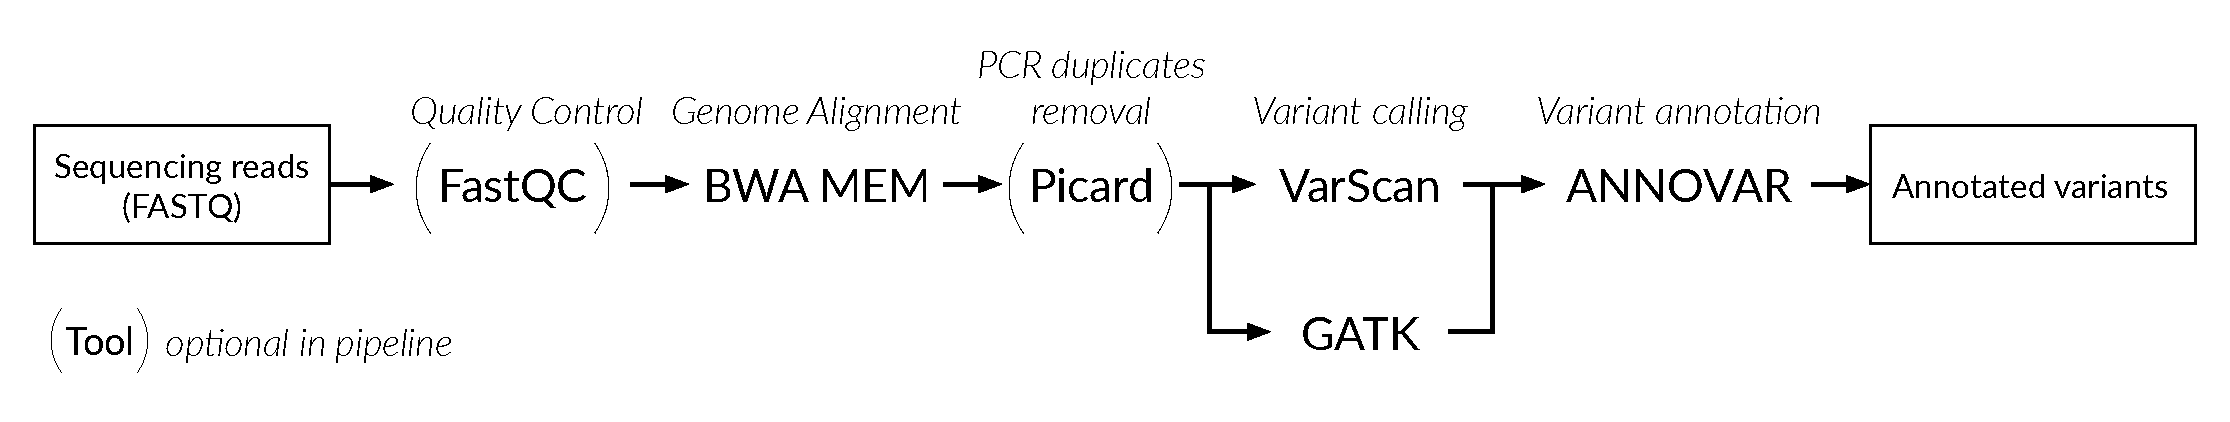
\includegraphics[width=\textwidth]{images/dnaseq_pipelines}
\caption[DNA-Seq analysis pipelines]{DNA-Seq analysis pipelines supported by BioCloud.}
\label{fig:dnaseq-pipeline}
\end{figure}


For variant calling, BioCloud supports two callers: VarScan
\cite{koboldt2012:varscan} and GATK
\cite{vanderauwera2013:fastq,mckenna2010:genome}. To use with VarScan, the
output alignment BAM file is processed by samtools' mpileup subcommand to
compare the aligned reads with genome reference sequence. VarScan take the
mpileup output and determine if it is a significant variant that beyond the
given threshold for each base. To use with GATK, the best practice
\cite{vanderauwera2013:fastq} made by \citeauthor{vanderauwera2013:fastq} is
adopted. However, since our lab does not use GATK for variant calling as
frequently as VarScan, the development to support GATK has been postponed.
Currently existed GATK protocols in our lab are for GATK 1.x, which are
outdated and are not compatible with the newer GATK 2.x.

After variant calling, these variants are further annotated with gene
information, SNP database records, animo acid and protein structure change
predictions by ANNOVAR \cite{wang2010:annovar}. ANNOVAR collects widely used
genome references such as refSeq and Ensembl, annotation databases such as 1000
Genome, dbSNP, ClinVar and COSMIC, and prediction algorithms such as SIFT and
PolyPhen-2. By relying on ANNOVAR, BioCloud don't need to look up each database
and reference on its own, which also reduces the maintaining burden for keeping
all database in use updated.



\section{BioCloud Website}
\label{s:biocloud-website}

In this section, the architecture of BioCloud website is introduced and an
overall picture is given. The workflow for generating summary report is
explained in Section~\ref{s:report-generation}. Except for summary report
generation, the mechanism of each component is explained per subsection,
including a message authentication method for access control and account
validation; experiment design for grouping samples in conditions and is reused
for multiple analyses; analysis submission with parameter settings; job queue;
and finally access control for report and results of an analysis.



\subsection{Overview}

Shown in Figure~\ref{fig:overview-arch}, BioCloud website can be viewed as
three main parts: data storage, computing cluster, and web frontend. For normal
user, they only interact with the web frontend and the architecture of BioCloud
will remain unknown for them. However, in the BioCloud internal structures,
these main parts can exist on different machines. So when large computing
resource is needed, more machines can be added to the computer cluster without
modifying the settings and source code of BioCloud. Data storage includes the
database and local file system to store data sources, genome references and
analysis results and reports. File systems like NFS can be used to allow access
from multiple machines if BioCloud operates across one and more servers.

\begin{figure}[!htb]
\centering
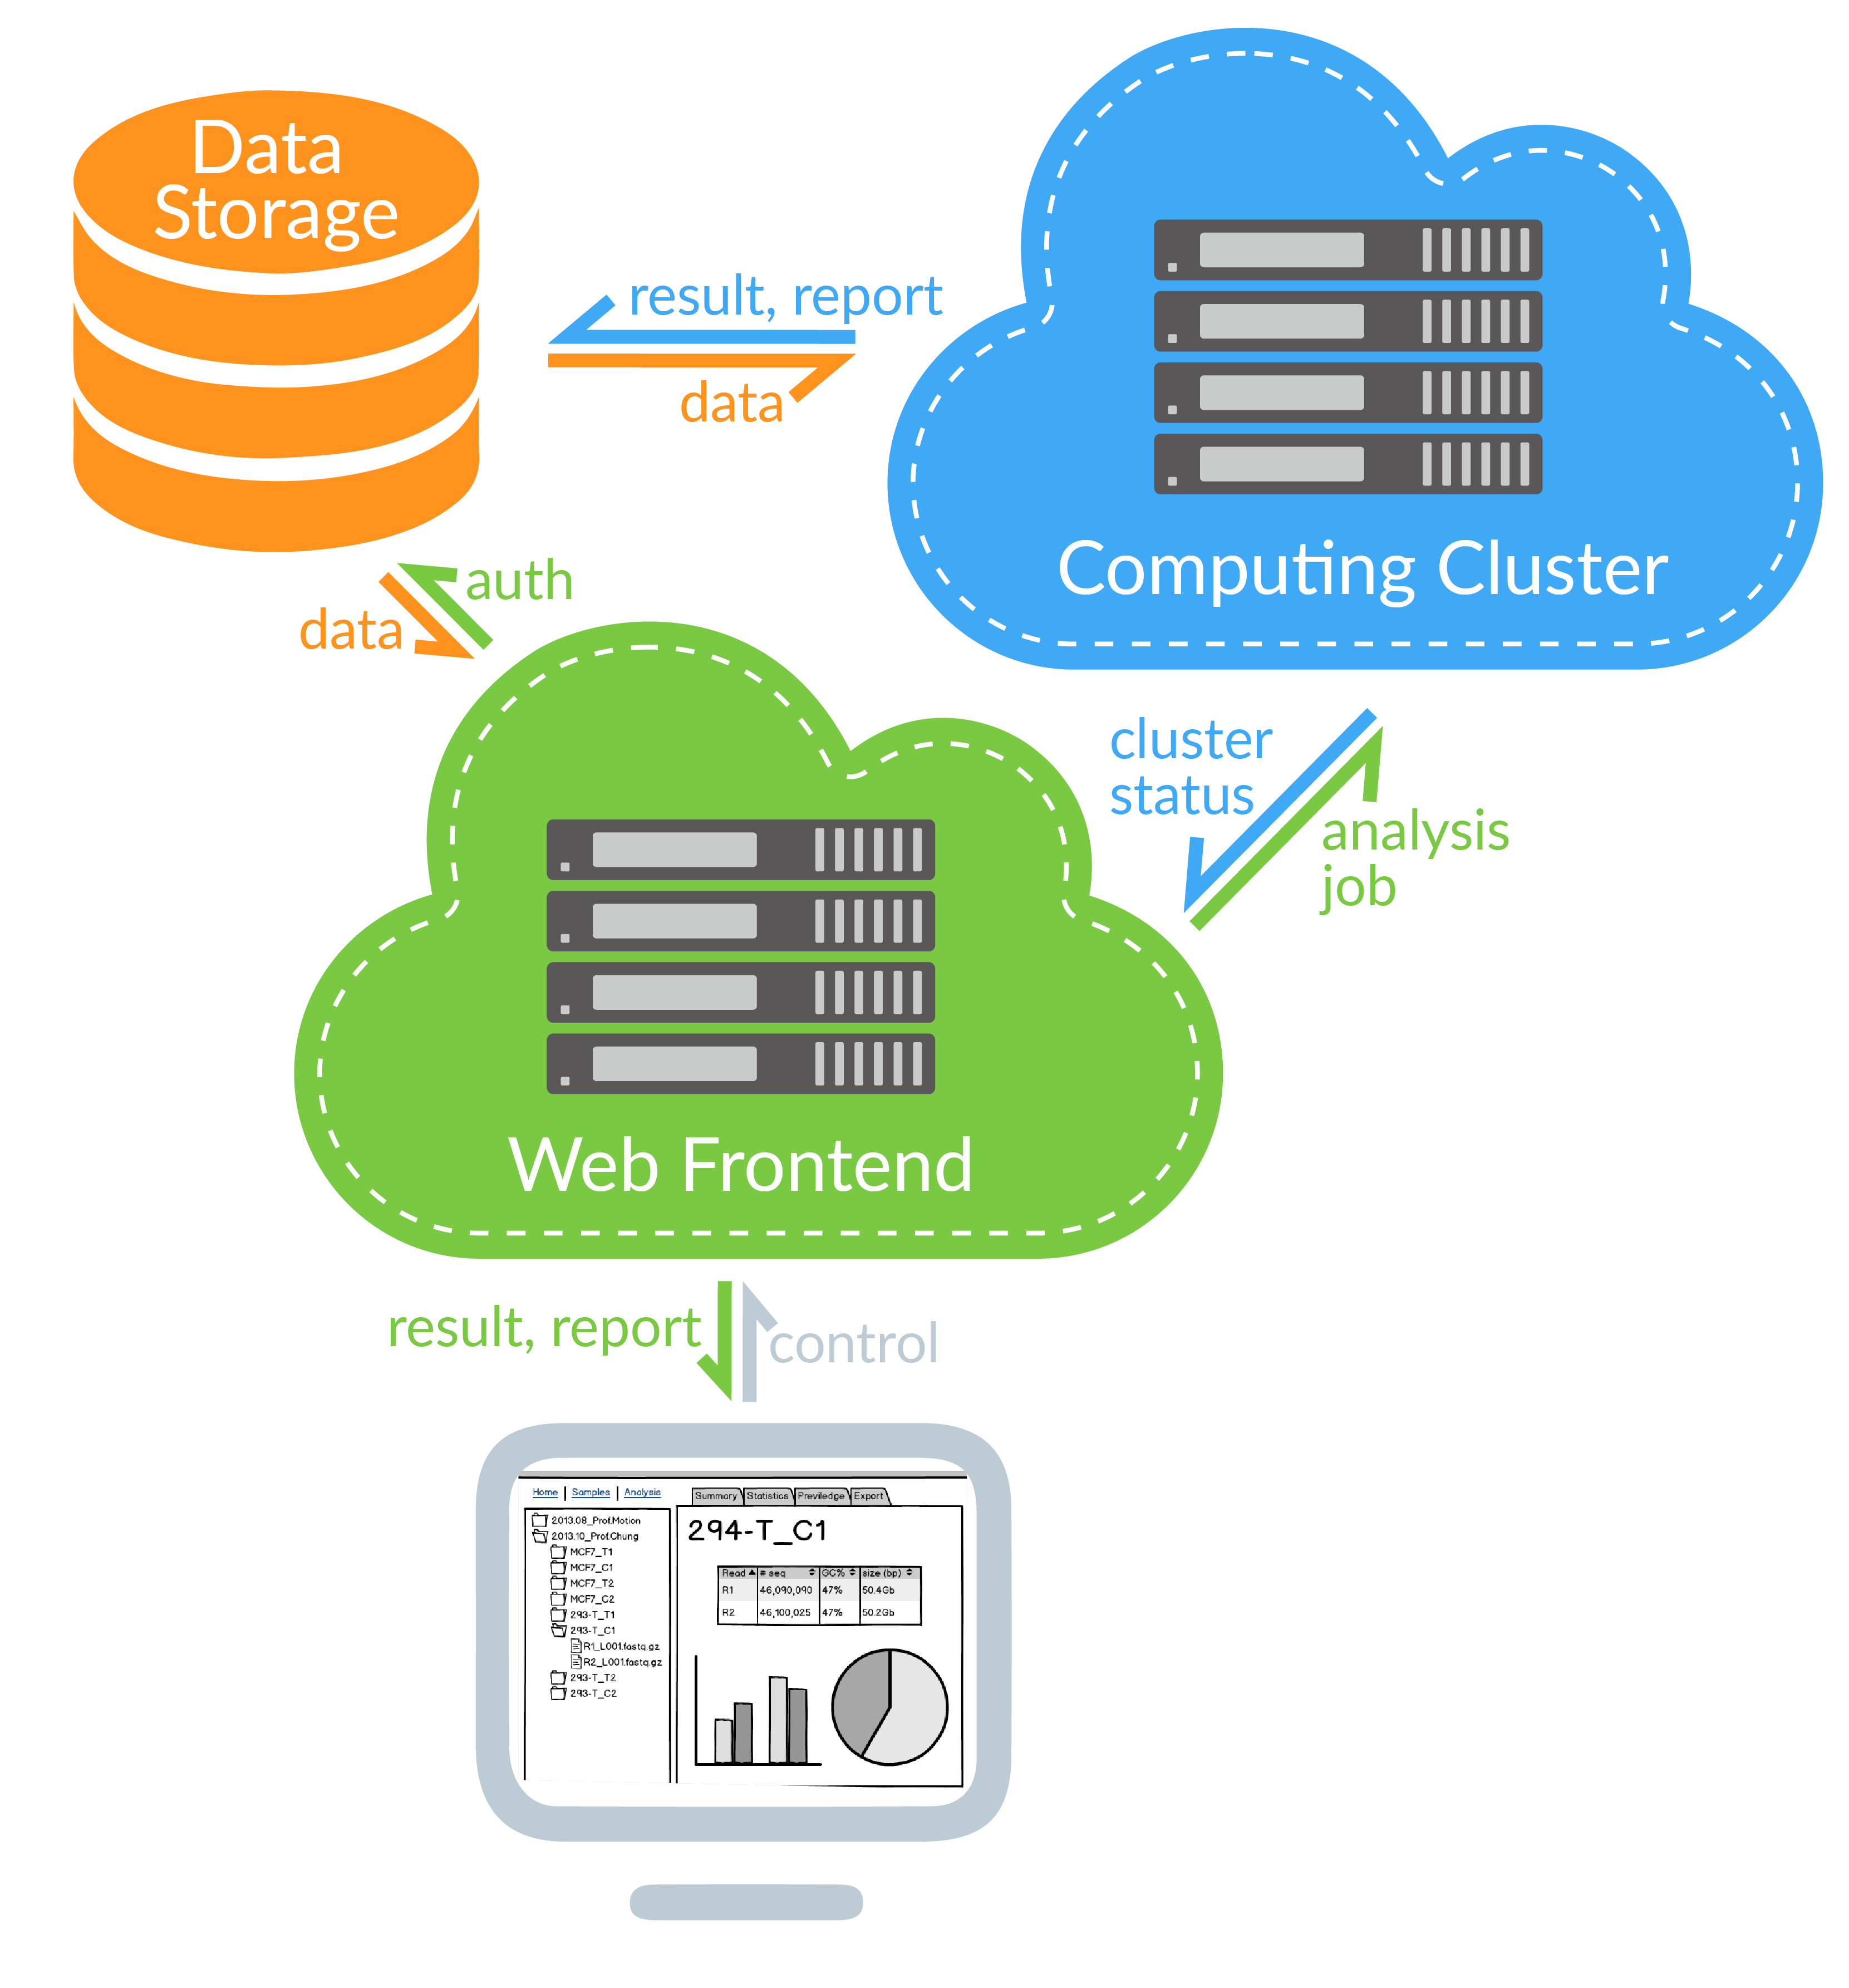
\includegraphics[width=0.75\textwidth]{images/overview_arch}
\caption[BioCloud overview architecture]{Overview of BioCloud architecture.}
\label{fig:overview-arch}
\end{figure}



We further breakdown this general BioCloud architecture into independently
operating components and demonstrate how these components interact in a
workflow of a user completing one analysis in
Figure~\ref{fig:overview-workflow}. Before going down the workflow explanation,
some terminologies BioCloud use should be clarified at first. A data source
represent an file on file system. A sample can be a collection of multiple data
sources. For example, a pair-end sequencing sample contains two data sources
corresponding to the R1 (or forward strand) and the R2 (or reversed strand) of
the sequencing result.

\begin{figure}[!tb]
\centering
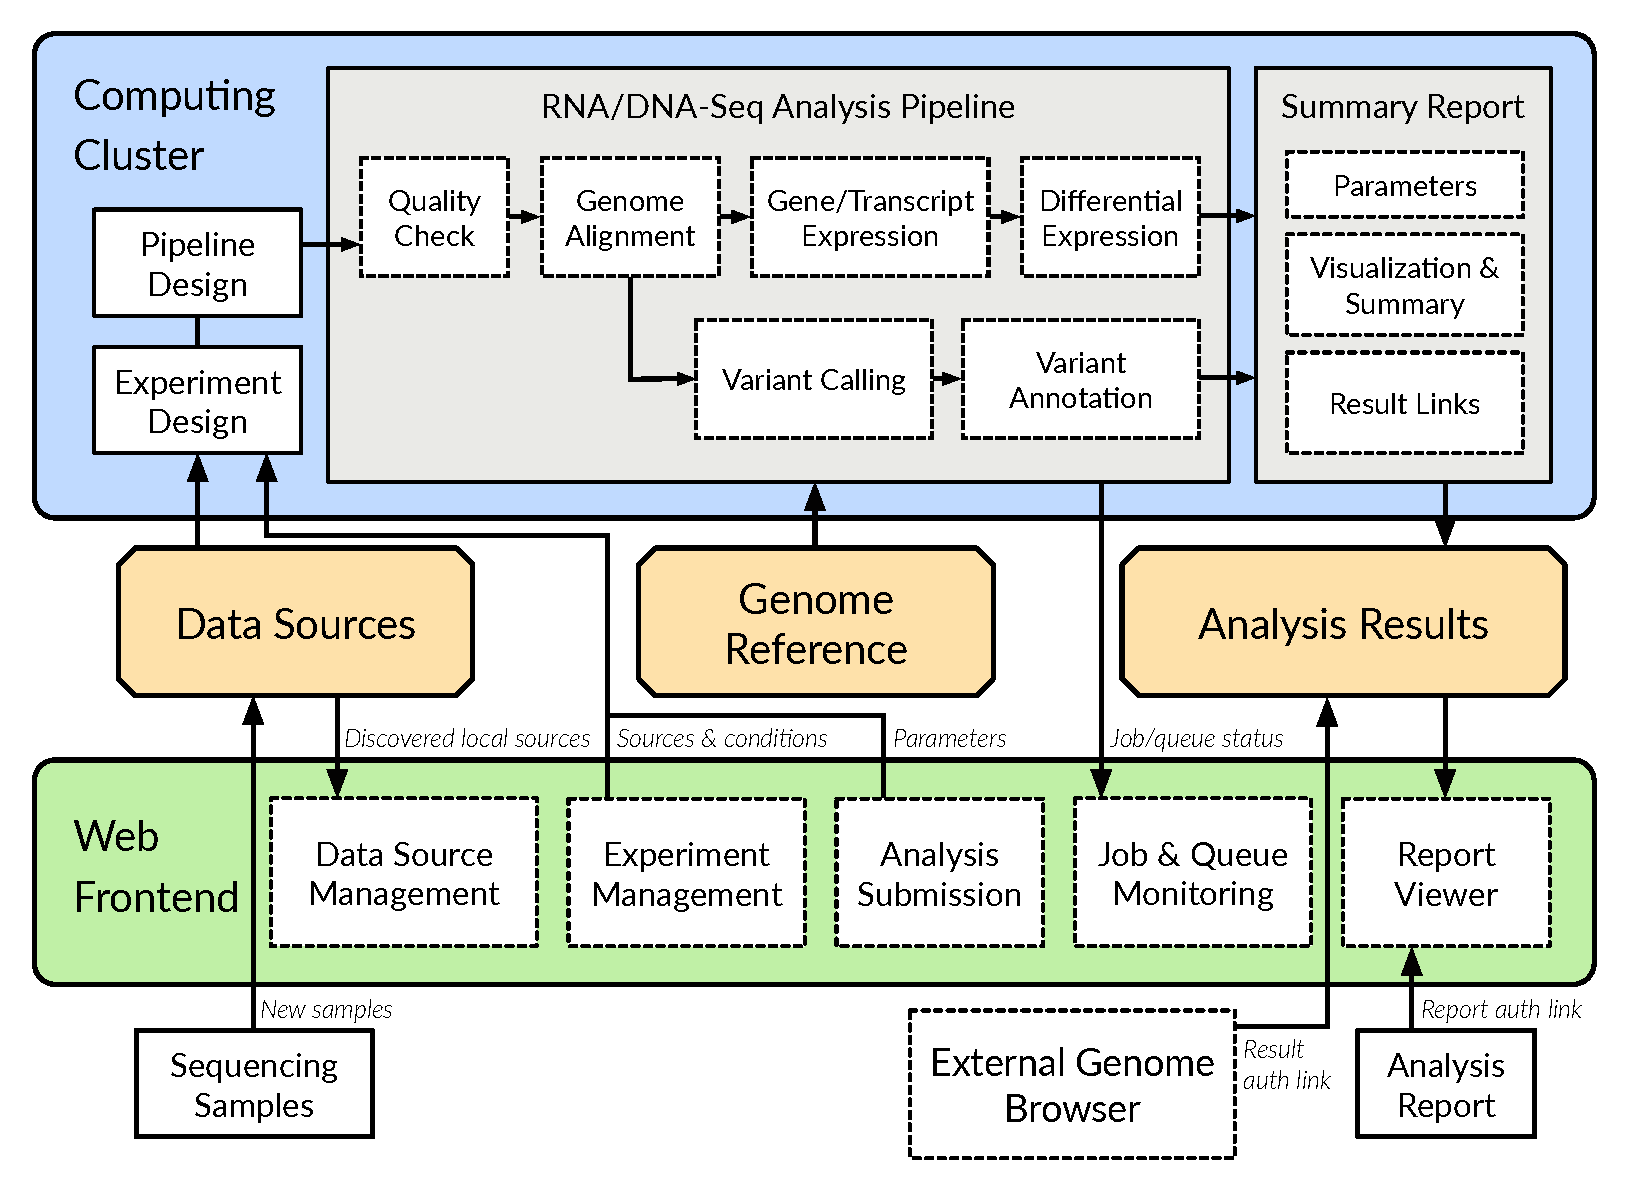
\includegraphics[width=1\textwidth]{images/overview_workflow}
\caption[Overview of BioCloud website workflow]{
    Overview of BioCloud workflow. All operations on data sources, experiments,
    and analysis require user login and thus are isolated by different user
    accounts.
}
\label{fig:overview-workflow}
\end{figure}


The journey of the analysis starts by adding new sequencing samples. These new
samples are added under the user's data source directory. During the auto
discovery, sample name, file type and other information of a source are guessed
by BioCloud but allowed for user to override them. An additional checksum can
be supplied for each source to confirm the data integrity. Data sources or
samples come in group of biological experiments. For example, a experiment can
have control group and test group with 4 samples each. In BioCloud we define
experiment as well, which is a collection of samples. In an experiment, each
selected sample is assigned a condition which can be used for grouping later-on
stages such as differential expression analysis. An experiment can be used in
one and more analyses such as trying different analysis parameters or using
different analysis pipeline. Therefore, an experiment contains which samples to
use and how they are grouped in terms of sample conditions.

Finally, user can now submit an analysis by specifying a pre-defined experiment
and tuning the parameters available for the chosen analysis. User is also
required to select the genome reference used for the analysis, whose possible
options include hg19 (UCSC), hg19 (Ensembl), and hg38 (NCBI). After configuring
and submitting the analysis, the analysis creates its corresponding job and
wait in the job queue for computing cluster to execute. Each analysis pipeline
defines its own unique sequence of execution stages. During the job execution,
the status of these stage reflect either a stage is successfully completed,
failed, running, skipped by user configuration, or waiting for the previous
stage to end. User can obtain the stage status through by monitoring jobs and
the queue. The summary report generation is automatically appended at the end
of each analysis, which is explained in Section~\ref{s:report-generation}. Once
the analysis completes, user will be notified by email with link to the
information page of the analysis.

User can view the summary report by the given link online. Also, outputs of all
executed tools are organized under the folder allocated for this analysis. User
can find the link to download these outputs as well. The report can be shared
to others without a BioCloud account by simply sharing the link. The link to
results and report can be set as private access or have a new URL if user does
not want to disclose their report and result anymore. By pasting the link to
results on genome browser like Ensembl and UCSC, user can immediately view
their results with other genome annotations without uploading full output file
to the genome browser.

\begin{figure}[htbp]
\centering
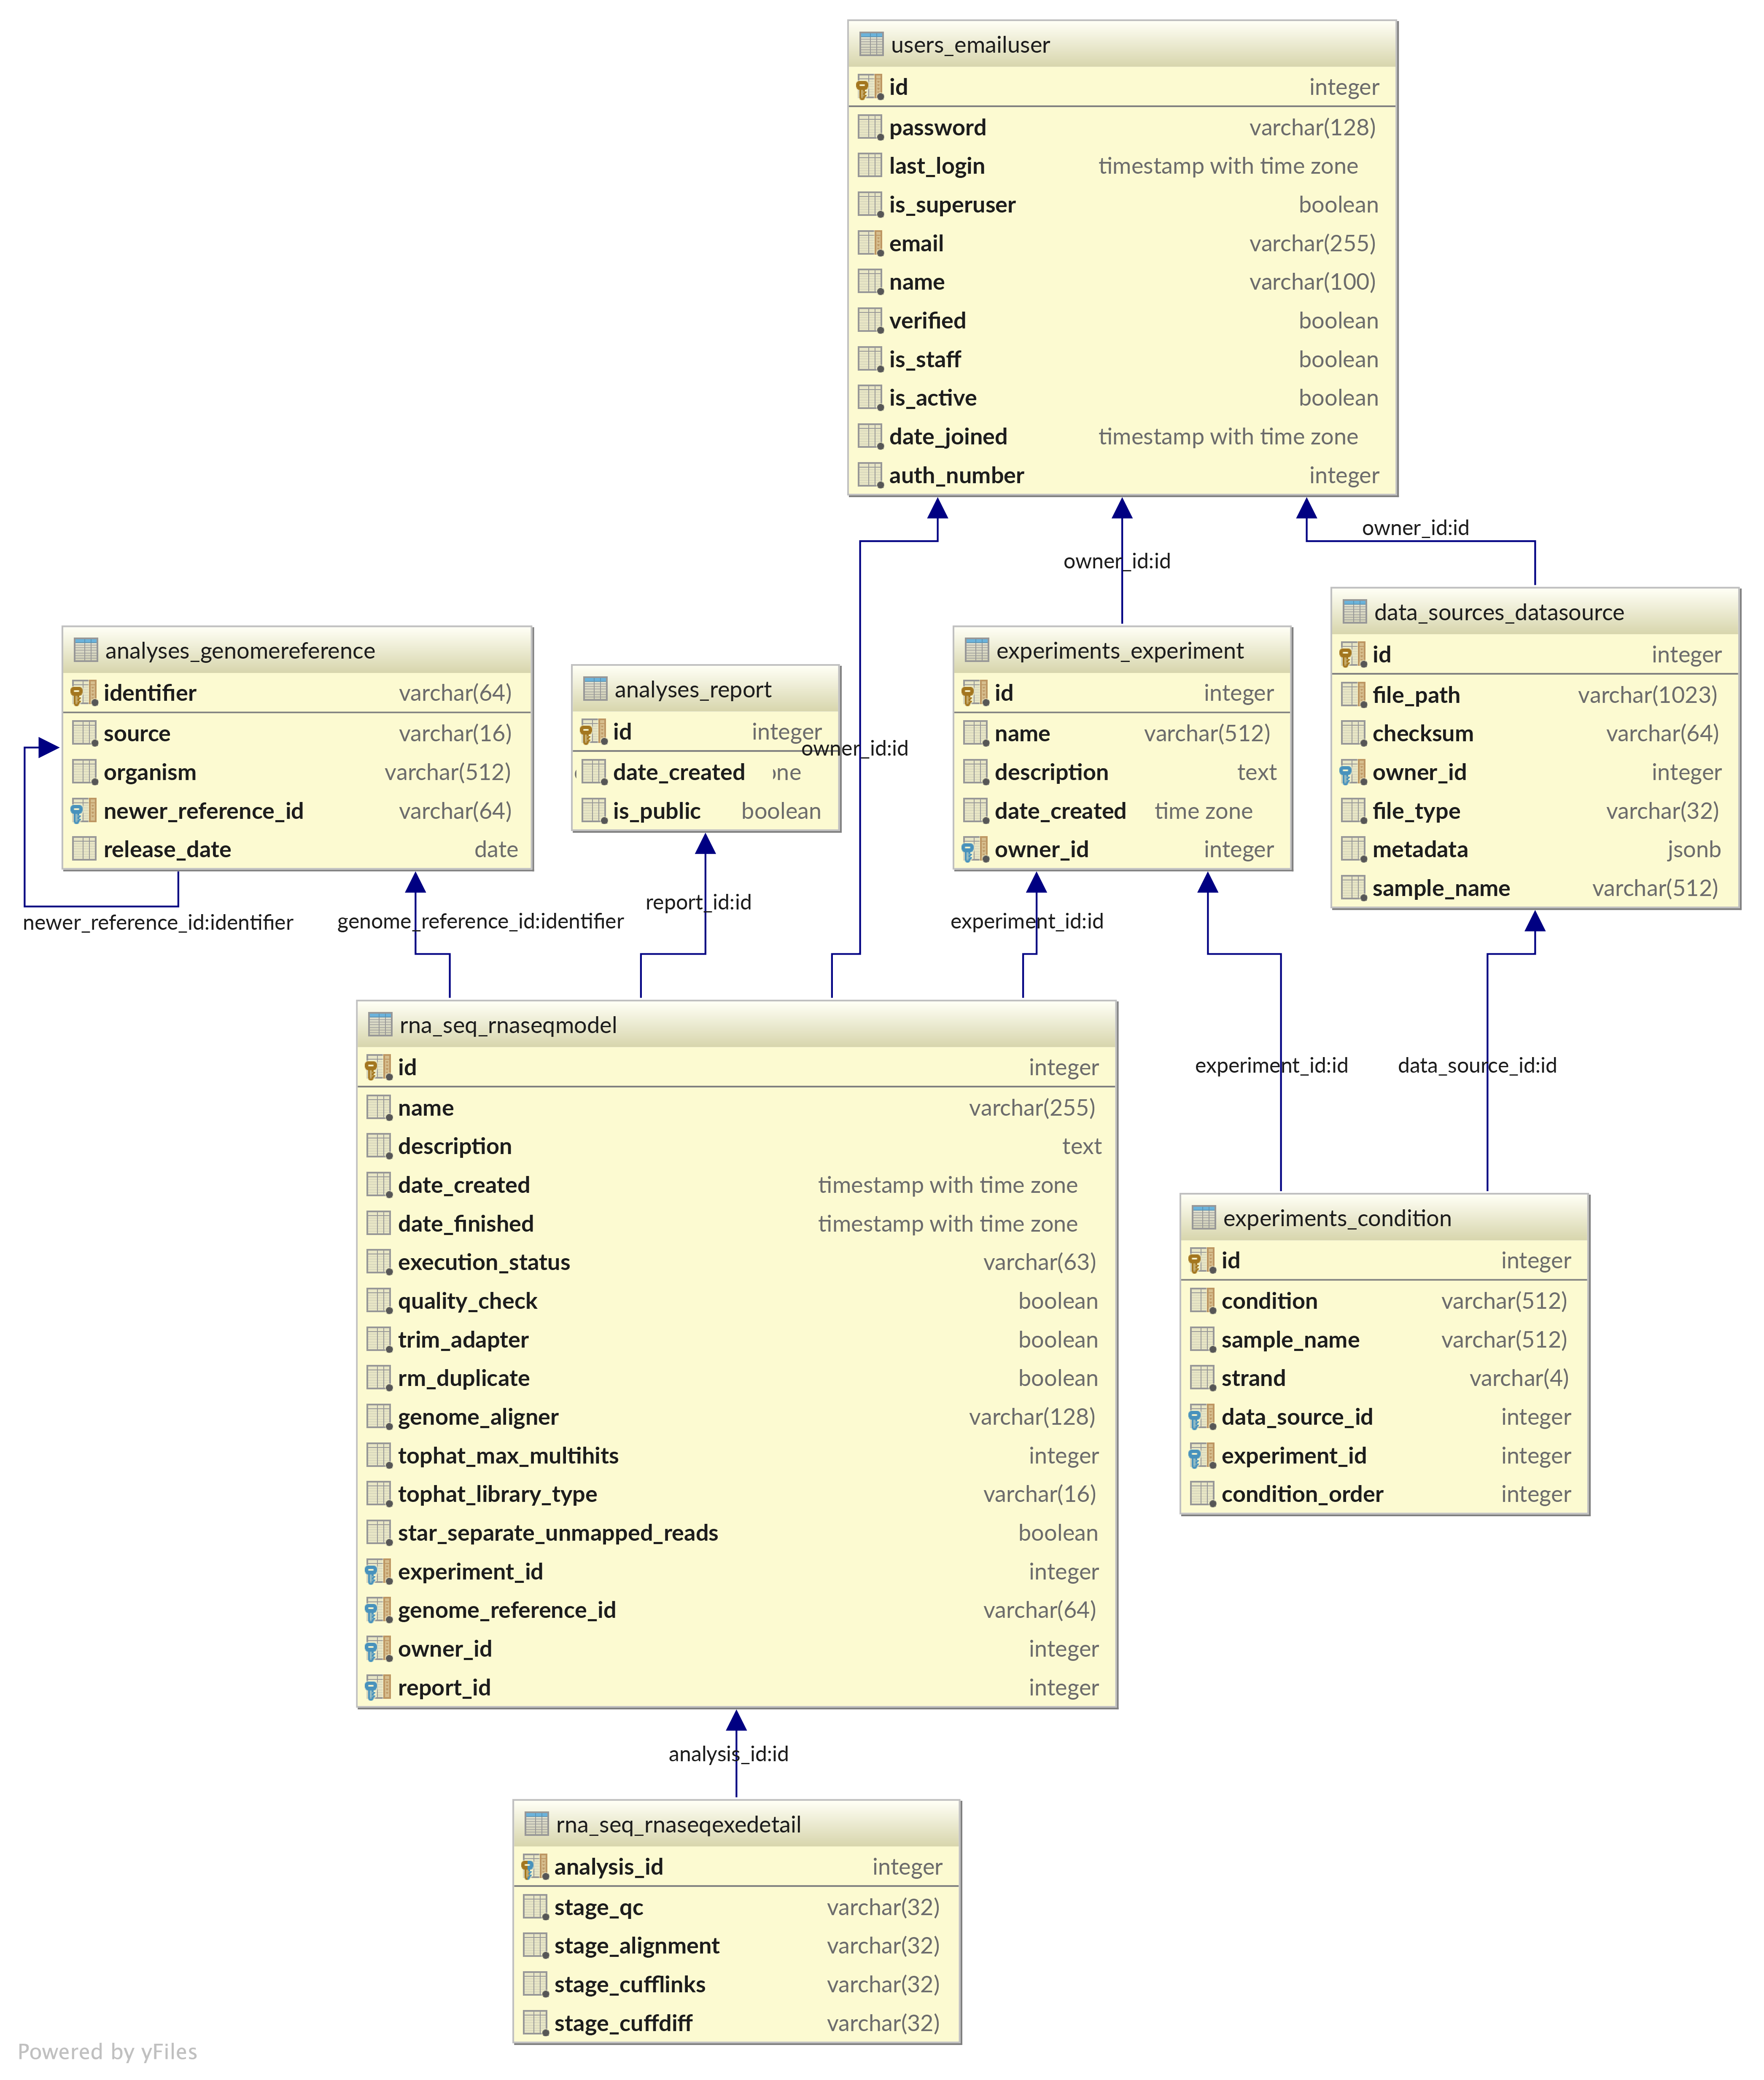
\includegraphics[width=\textwidth]{images/biocloud_erd}
\caption[Entity relation diagram (ERD) of BioCloud database]{
    Entity relation diagram (ERD) of BioCloud database. Here only one analysis
    pipeline of RNA-Seq (table \texttt{rna\_seq\_rnaseqmodel}) is shown for
    simplicity. Tables related with Django web framework internals and job
    queue framework are also omitted.
}
\label{fig:biocloud-erd}
\end{figure}


So far all major components of BioCloud have been covered and they will be
explained in detail in the following subsections. The corresponding database
design is shown in Figure~\ref{fig:biocloud-erd}.


\subsection{Data integrity check and authentication}

Data integrity check and authentication are important topics in BioCloud
website. Data sources need to be checked if the content of uploaded file is
identical to that of user's local copy. During account activation, an unique
activation link for this account is generated and sent to the email registered
by the account. When the user clicks the link, BioCloud knows which account is
activated and is certain that user actually posses this email address. For
sharing report or result through given link, BioCloud verify the link is valid
and retrieve the corresponding analysis report or result. Except for data
integrity check, we have to make sure all the links mentioned above cannot be
forged in a reasonable time given the current computing power. Therefore, in
BioCloud several methods are used to make sure the data integrity and to
validate authentication link and code.

To check data integrity of upload data sources, a checksum per file using
SHA2-256 hash algorithm can be passed during the data source discovery can be
provided. Checksum summarizes the file into a fixed length of bits no matter of
the file size. The checksum algorithm is sensitive to minor changes, so if a
file have a few bytes corrupted during the network transmission, its checksum
will be drastically different to the correct counterpart. Checksum is not file
compression so it can only be used for data integrity check. The checksum of
two different files can be identical, the incident being referred to as
collision. The checksum algorithm in use, SHA2-256, generates 256bits long
checksum.

For authentication, hash-based message authentication code (HMAC) is used to
create the authentication key. A HMAC string consists of two parts: the
original message and a signature for the original message, which is generated
with a secret key and a salt string in the current BioCloud implementation. The
signature is a hash is generated based on the given secret key concatenating to
salt string and the original message. Since the secret key is not disclosed to
user, knowing the original message and the salt string cannot re-create the
signature. The only way to forge the signature is through hash collision.
However, by choosing cryptographic hash function such as SHA-1\footnote{
    SHA-1 is not considered collision resistant anymore, though it is still
    suitable to be used as the hash function of HMAC.
} and SHA-2, they are collision resistant so it is hard to find a collision
in feasible time. The salt key, public or private, extends the computation
effort to crack the underlying secret key. By passing JSON as the original
message, one can store complex data structure in one HMAC string.


\subsection{User account management}

To let individuals manage their own data sources, analyses and results,
BioCloud builds its user account management based on Django's implementation.
Security is one of the top concern for BioCloud, we rely on the password
management made by Django which is secure and long tested in the public.
BioCloud requires email and password for registration.

Since it sends out email notification to users, the email address is first
verified by sending an activation link upon registration. The link contains a
HMAC token consisting of user's email address and registration timestamp. The
timestamp can verify if the activation link has been expired. The activation
link is generated on-the-go when a user requests. Compared to alternative
solution to store activation links in the database, our approach does little
performance impact on database system. A user is marked as verified once the
account activation is complete.

To better maintain the BioCloud, special account types, staff and superuser
account, can access to the BioCloud admin interface and view and modify all
users' data and activities. Superuser doesn't need to permission to do all
operations in the admin interface, whereas staff can only performance a subset
of granted operations. The account type can be adjusted by
\texttt{is\_superuser} and \texttt{is\_staff} columns of
\texttt{users\_emailuser} table, as shown in Figure~\ref{fig:biocloud-erd}.
User's data sources and experiments, and analyses are referred back to its user
record via \texttt{owner\_id} column on their respective table.


\subsection{Data source management}

Once the account is initiated, BioCloud create a folder for user to store
data sources based on the user ID. User ID is auto generated and unique. User
can either move or link their data sources under this folder.

User then add these data sources using ``data source discovery'' function of
BioCloud. It scans user's data source folder and filter newly added sources
with the user's database records. Sample name and type of the data source is
guessed by BioCloud. After the discovery, user can override the guessed values
and add checksum for each discovered files. User can later change these
property after the data sources are added as well.

The representation of data source in the database is a straight-forward
mapping, as table \texttt{data\_sources\_datasource} shown in
Figure~\ref{fig:biocloud-erd}. However, there are some metadata that are only
required for certain file types. For example, only FASTA and FASTQ files can be
pair-end, e.g., R1 and R2. Metadata is stored as a column of JSON type.
Metadata can be a hierarchical data structure in one column and database won't
complain if some substructure of a metadata record cannot be found in another.


\subsection{Experiment design}

Experiment collects a group of data sources and labels them with conditions. An
example of experiment design is shown in Table~\ref{tab:experiment-example}. In
this experiment, four samples, A, B, C and D, from user ID 1 with pair-end
FASTQ files, are selected. The former two samples are of condition control,
while rest of the samples are of condition testing.

\begin{table}[!htb]
    \caption[Example of experiment design]{Example of experiment design.}
    \label{tab:experiment-example}
    \centering
    \begin{threeparttable}
        \begin{tabular}{ccrr}
            \toprule
            Condition & Sample name & Forward read (R1) & Reversed read (R2) \\
            \midrule
            Control & A & \texttt{1/A\_1.fastq} & \texttt{1/A\_2.fastq} \\
            Control & B & \texttt{1/B\_1.fastq} & \texttt{1/B\_2.fastq} \\
            Testing & C & \texttt{1/C\_1.fastq} & \texttt{1/C\_2.fastq} \\
            Testing & D & \texttt{1/D\_1.fastq} & \texttt{1/D\_2.fastq} \\
            \bottomrule
        \end{tabular}
    \end{threeparttable}
\end{table}


BioCloud creates an interactive frontend for user to filter and select the data
sources they want to include in this experiment. Since a simple may have
multiple data sources, by default BioCloud guesses using the sample information
during discovery. However, user can override the sample name during experiment
design. For example, user can create a new sample called AC and include all
four data sources originally of sample A and C. After finalizing the samples,
user defines the available conditions for this experiment and assign sample to
them.

To sum up, there are three steps to design an experiment: select data sources,
label sample name on data sources, label condition on samples. However, user
can freely go back and modify result of the previous stage. BioCloud will try
to re-use all user given information maximally as possible so user don't need
to re-fill all the information again. For example, if the condition ``Control''
is misspelled as ``Contorl'', when updating the condition name, all samples of
the condition will remain and their condition names will be updated
simultaneously. BioCloud achieves this feature by binding condition and sample
name only on data sources' metadata, and user updates directly to the metadata.
When a metadata is changed, BioCloud decides which part of the experiment
design is changed and re-renders all the affected output. This is the notion of
web frontend development called reactive programming.

User can give experiment name and description to help manage all defined
experiments. Description is written in Markdown syntax \cite{:commonmark},
which is a lightweight markup language that convert plain texts into styled
document. Users are encouraged to put relevant links and references regarding
to the experiment in its description. Once an experiment is created, user will
no be able to modify the condition and sample design. The fixation of
experiment design ensures all analyses depending on it will have the same
setting of conditions and samples.


\subsection{Genome reference}

Genome reference store all related references and annotations for a given
version of genome reference. For human, there are hg38 (UCSC), hg38 (Ensembl
Release v84), and hg19 (UCSC); for mouse, there are mm10 (UCSC) and mm10
(Ensembl v84). All tools required index files and the annotations should be
available for every supported genome reference. For example, if one decides to
support hg38 (UCSC) genome reference, all aligners' genome index including
HISAT2, STAR, Bowtie and BWA needs to be generated; dbSNP needs to be version
141 and latter to support hg38 genome reference. It should be noted that
primary assembly of genome won't change across patch releases. So primary
assembly sequence of GRCh38 and GRCh38.p5 remain the same.

Genome reference are managed via the table
\texttt{analyses\_genomereference} using BioCloud admin interface. By providing
the release data of the genome reference, BioCloud can sort the reference in
chronological order. If a newer genome reference comes out, one can specify the
upgrade path in the column \texttt{newer\_reference\_id} so downstream analysis
tools can provide a better hint to user about the new genome reference release.
Genome references are all stored under a same folder specified through the
BioCloud's setting file. Its internal folder structure resembles that of
iGenome \cite{:igenomes}.


\subsection{Analysis submission}

A new submission analysis requires selection of analysis pipeline type and
experiment design. First user selects one of the analysis pipelines described
in Section~\ref{s:rnaseq-pipeline} and \ref{s:dnaseq-pipeline}. After an
analysis is chosen, the webpage is directed to the corresponding form page to
adjust the analysis parameters. There are some common parameters for all
analyses pipelines, including name, description, genome reference and
experiment in use. Like the description of experiment, description of analysis
is written in Markdown to provide basic markups like hyperlinks and bullet
lists. When choosing the experiment, its condition and sample design is shown
dynamically.

Parameters of an analysis pipeline include the choose of tools of equivalent
function and parameters passing to the chosen tools. As shown in the
Figure~\ref{fig:biocloud-erd}, a RNA-Seq pipeline analysis that uses Cufflinks
for differential expression analysis. All of the possible parameters are
stored as separate columns. However, only a subset of the parameters will be
used, mainly depending on the genome aligner user chooses (user's choice is stored
at \texttt{genome\_aligner} column). To avoid user confusion, the form that
renders the analysis parameters will dynamically display the corresponding
parameter set given user's choices. For example, if user chooses HISAT2 as the
genome aligner, all options for Tophat2 and STAR will be hidden. The dynamic
display rendering is also handled by reactive programming in web frontend.


\subsection{Job queue management}

% describe what happens when a new analysis is submitted
% - analysis detail created (stage)
% - report and result directory created
% - mark the analysis as queueing

As a new analysis is submitted by user, it first initiates extra settings to
describe the job execution detail, e.g., stage status, and allocate folders to
store the result and report of the analysis. A job execution detail group an
analysis pipeline into execution stages, whose status can be waiting, running,
successful, failed, or skipped. Take the example RNA-Seq analysis pipeline
shown in Figure~\ref{fig:biocloud-erd}. Its job execution detail is stored in
table \texttt{rna\_seq\_rnaseqexedetail} and defines four stages: qc,
alignment, cufflinks, and cuffdiff. If user opts out quality
check upon setting the analysis, it won't execute FastQC and the qc stage will
be marked as skipped. Stage status will be shown when user query about the
current analysis execution status. Additionally, new analysis will create a new
report record with an unique ID. This ID may differ with the analysis ID since
same analysis ID may appear in different types of analysis pipelines. Folder
for result and report of the analysis will be created based on the report ID.
Finally, the analysis execution status is marked as queueing and wait for a
work of the computer cluster to pick up.

% computer cluster job queue and worker
% - get the analysis ID
% - one machine only have one worker

Computer cluster runs its job queue and job workers in separate processes. The
queue monitor continuously watches if a new job, e.g. a new analysis, is added
to the job queue. When a new job is added, it pass down to one of its available
worker to execute. The job queue BioCloud uses guarantees at least once
delivery. The job worker receives a new job with the analysis ID and obtains
all related information by querying the database with this analysis ID. Here
the analysis ID is used for analysis of different pipelines won't share the
task they run so no ID collision issue. During the execution, work updates the
stage status in the way previously mentioned. When the analysis is completed
and the summary report is generated, the worker will notify the user about the
completion via email.


\subsection{Report and result access control}

% what is in the report HMAC token
% - email, auth number, report ID
% no login for this link set the report link as public or private change the
% report HMAC token canonical link to the report
To enable report and result sharing, HMAC token is used to control the access.
The access URL patterns for a report and the result file of the same analysis
are shown in the following, which share the same authentication key
\texttt{<auth key>}:

\begin{CVerbatim}[fontsize=\small]
https://<biocloud domain>/access/<auth key>/report/
https://<biocloud domain>/access/<auth key>/result/path/to/file
\end{CVerbatim}

\vspace{-1em}\noindent
Access to the report and result files via these URLs does not require the
viewer to be logged in on BioCloud or to be the owner of the analysis.

Authentication key contains the user's email, a customizable authentication
number, and the report ID. The user's email is used to prevent user on BioCloud
from forging access to other user's report easily. Authentication number is
decided per user which can be modified in the user profile setting. If the
number is changed, all authentication keys of this user will be updated and
invalidate the previous ones. The number is useful when user accidentally
disclose one's report or result link in public or user finishes connecting the
data with external genome browser. Finally, the report ID is stored in the
authentication key so BioCloud understands which report to retrieve. Aside from
the key, user can control to let individual report to be public or private.

When the BioCloud server receives a request for a report or a result file, it
first validates the authentication key and extract the report ID. If the key is
invalid, a HTTP 404 error of invalid access is raised. Upon any check below
fails, the same HTTP 404 error is raised. If the key is valid, it further
checks if the current authentication number of user match the one extracted
from the key. Then, it checks if the requested report is public or private. For
private report, viewer must be already logged in and must be the owner of the
report. After all above checks are passed, BioCloud serves the report content
or the result file specified by the rest of the URL.

Since the report and result link can be changed frequently, BioCloud also
provide a canonical access link for report, which redirects user to the
currently valid report URL, shown in the following:

\begin{CVerbatim}[fontsize=\small]
https://<biocloud domain>/access/report/<report ID>/
\end{CVerbatim}

\vspace{-1em}\noindent
Only the logged in owner of the report can use the canonical link, so it cannot
be shared with others.



\section{Report generation}
\label{s:report-generation}

Summary report shown in Figure~\ref{fig:overview-workflow} is generated after
an analysis job finishes. A more detailed report generation workflow is shown
in Figure~\ref{fig:bcreport-workflow}. A standalone program, BCReport, that
parses a set of results of NGS analysis tools and generates the summary report.
By specifying the structure of data sources, samples and conditions, BCReport
can provide summary report for any results which need not to be generated on
BioCloud. The standalone mode of BCReport extends the ability to parse a more
general set of NGS results. Moreover, for tools that BCReport does not support,
developers can extend the currently available report templates and result
parsers to build their own analysis pipelines.

\begin{figure}[!p]
\centering
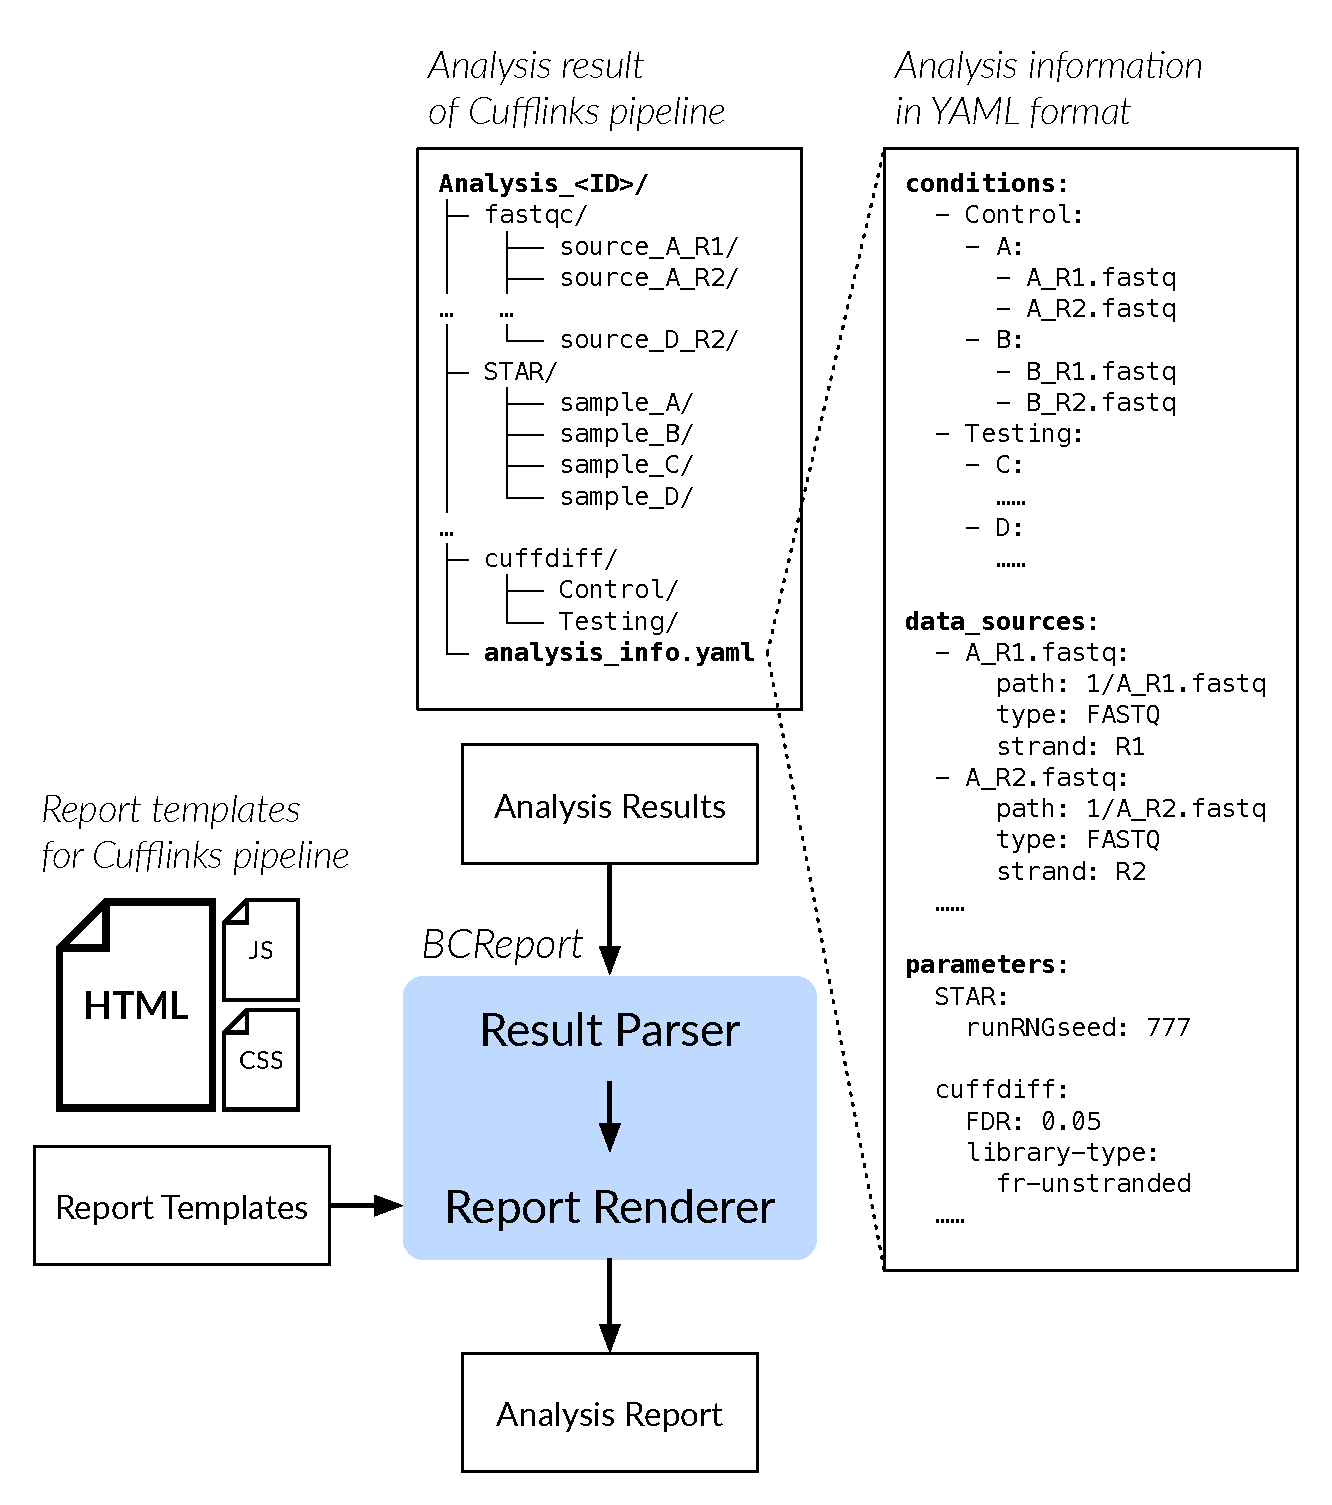
\includegraphics[width=1\textwidth]{images/bcreport_workflow}
\caption[BioCloud report (BCReport) generation workflow]{
    BioCloud report generation workflow. A standalone program, BCReport,
    hanldes the report generation process. BCReport reads the analysis info in
    YAML format and the result folders to understande how the analysis was
    executed. Then it parse the result folders using the parser for the
    corresponding analysis pipeline to extract the important information used
    in summary report. Finally, summary report is rendered based on the
    pre-defined ptemplates.
}
\label{fig:bcreport-workflow}
\end{figure}




\subsection{Analysis result strucntion and information}

A result folder structure readable for BCReport is shown in
Figure~\ref{fig:bcreport-workflow}, where each tool allocates its own result
folder. The folder name for the result of a tool can be flexible. For example,
for folder that contains result of STAR, its name can be \texttt{STAR} or
\texttt{2\_STAR}. Numerical prefix can help file system sort the result folders
to reflect their execution order. Inside the result folder of a tool, there are
four main types of grouping structure: by data sources, by samples, by
conditions and no grouping structure at all. The grouping structure depends on
the execution type of tool. For example, FASTQ runs quality check per data
source, thus its results are grouped by data sources; STAR runs alignment per
sample; Cuffdiff runs differential expression analysis and outputs the result
per condition; Cuffmerge combines transcript annotations of all samples and
produces one output for an analysis. BCReport's tool parser understands how
each tool is executed and will parse its result based on the corresponding type
of grouping structure.

% result folder structure
% analysis inform in YAML
%   data source, sample, conditions, parameters

To let BCReport understand how the analysis was executed, analysis information
including data sources, samples, conditions, and tool parameters are stored in
an analysis information file \texttt{analysis\_info.yaml} in YAML \cite{:yaml}
format. As shown in the Figure~\ref{fig:bcreport-workflow}, there are three
sections of the analysis information: conditions, data sources, and parameters.
In conditions section, grouping of samples and conditions are specified. In
data sources section, the detail of all data sources in use is given. In
parameters section, tool parameters specified during analysis submission are
recorded. Additional analysis information will be places in this section as
well.

As long as the analysis results are organized in the folder structure stated
above and an analysis information YAML file is provides, BCReport can recognize
the analysis and provide the summary report. However, when BCReport is used
with BioCloud, it can also retrieve the raw data access links from BioCloud and
display them in the summary report.



\subsection{BCReport: result processing framework}

% HTML template rendering
When the BCReport is called, it first parses the analysis results based on the
analysis information. An additional parameter is passed to instruct BCReport
which analysis pipeline parser is used to extract the given analysis result. An
analysis pipeline parser contains the logics to extract the result and the
corresponding templates to display. Since an analysis pipeline may have
different tool execution branches, the template rendering contains conditional
blocks so only chosen tools will be processed. For example, for a analysis
based on Cufflinks RNA-Seq pipeline described in
Figure~\ref{fig:rnaseq-pipeline}, there are three possible genome aligners.
Based on the analysis result shown in Figure~\ref{fig:bcreport-workflow}, STAR
is used for genome alignment. Therefore, result sections about Tophat2 and
HISAT2 will be skipped and not shown in the summary report. However, to prevent
unnecessary complexity in the analysis pipeline design, users are not
encouraged to create too many execution branches in a pipeline. When used with
BioCloud, BioCloud set a special flag of BCReport to display the URLs to
original data files. These URLs will contain the valid access token.

All tools defined in current BioCloud analysis pipelines can be re-used by
users to design new custom analysis pipeline. The extension on existed pipeline
is discussed in Section~\ref{s:pipeline-extension}.


\section{Implementation}

\subsection{Website}


% Django
% Django-Q
% Vue.js


% database
BioCloud code base communicates with the database via Object-relational Mapping
(ORM), which continually checks with consistency between the database scheme
and the mapped object representation in source code.

% vue.js
\begin{figure}[!htb]
\centering
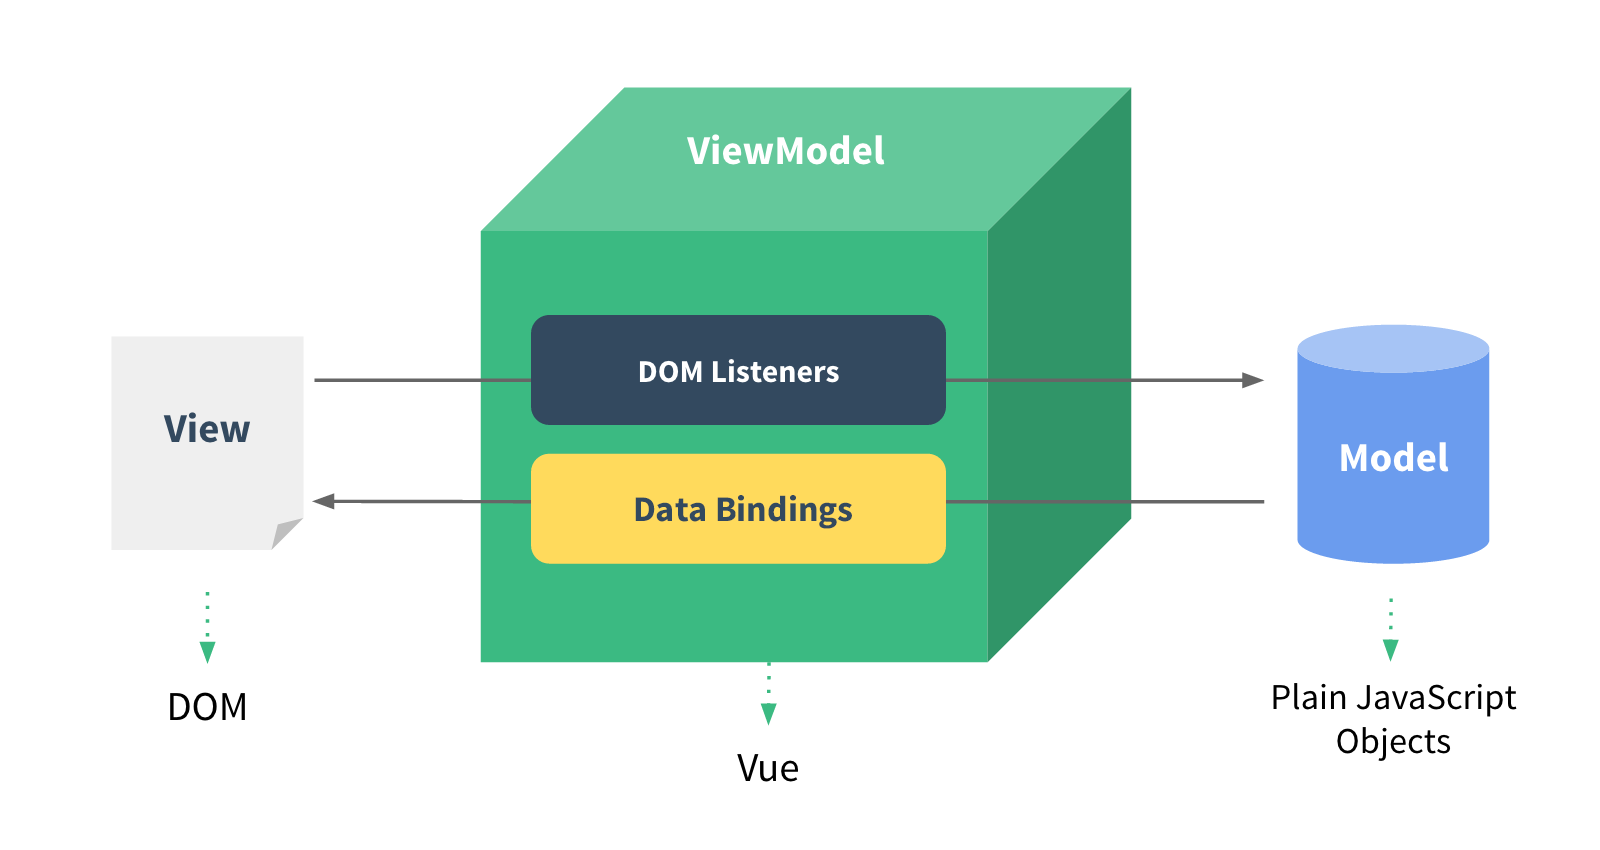
\includegraphics[width=0.8\textwidth]{images/vuejs_mvvm}
\caption[Reactive data binding diagram of Vue.js]{
    Reactive data binding diagram of Vue.js. The diagram is obtained from the
    \href{https://vuejs.org/guide/overview.html}{Vue.js official tutorial}.
}
\label{fig:vuejs-mvvm}
\end{figure}



\subsection{Deployment}

% nginx systemd
% nginx x-Accel and Django auth integration

\subsection{Report}

% YAML
% Jinja2
% skbio
% Vue.js
% plotting libraries

% vim: set textwidth=79:

\chapter{Results}
\label{c:result}

\section{Datasets}
\label{s:dataset}

%
% GSE52194 Breast cancer
% GSE52778 Airway Muscle and Asthma
%

Two RNA-Seq datasets and one DNA-Seq datasets from Gene Expression Omnibus
(GEO) were used for the demonstration of BioCloud. GSE52194
\cite{eswaran2012:transcriptomic} was a transcriptome profiling dataset of
human breast cancer. mRNA profiles of 17 breast tumor samples of three
different subtypes (TNBC, non-TNBC and HER2-positive) and normal human breast
organoids (epithelium) samples (NBS) were sequenced using Illumina HiSeq 2000
sequencer. Full sample list can be found in Table~\ref{tab:dataset-breast}.
Raw sequence reads were obtained from NCBI Sequence Read Archive (SRA), thus
their FASTQ file names were based on their SRA accession ID. In GSE52194 breast
cancer dataset, condition was defined to be the cancer subtype of the sample.

\begin{table}[!htbp]
    \caption[Experiment design of breast cancer GSE52194]{
        Experiment design of breast cancer dataset GSE52194.
    }
    \label{tab:dataset-breast}
    \centering
    \begin{threeparttable}
        \begin{tabular}{llr}
            \toprule
            Condition & Sample name & SRA ID and filename \\
            \midrule
            NBS      & NBS1      & SRR1027188 \\
            NBS      & NBS2      & SRR1027189 \\
            NBS      & NBS3      & SRR1027190 \\
            TNBC     & TNBC1     & SRR1027171 \\
            TNBC     & TNBC2     & SRR1027172 \\
            TNBC     & TNBC3     & SRR1027173 \\
            TNBC     & TNBC4     & SRR1027174 \\
            TNBC     & TNBC5     & SRR1027175 \\
            TNBC     & TNBC6     & SRR1027176 \\
            Non-TNBC & Non-TNBC1 & SRR1027177 \\
            Non-TNBC & Non-TNBC2 & SRR1027178 \\
            Non-TNBC & Non-TNBC3 & SRR1027179 \\
            Non-TNBC & Non-TNBC4 & SRR1027180 \\
            Non-TNBC & Non-TNBC5 & SRR1027181 \\
            Non-TNBC & Non-TNBC6 & SRR1027182 \\
            HER2     & HER2-1    & SRR1027183 \\
            HER2     & HER2-2    & SRR1027184 \\
            HER2     & HER2-3    & SRR1027185 \\
            HER2     & HER2-4    & SRR1027186 \\
            HER2     & HER2-5    & SRR1027187 \\
            \bottomrule
        \end{tabular}
    \end{threeparttable}
\end{table}


Another RNA-Seq dataset, GSE52778 \cite{himes2014:rnaseq}, is a transcriptome
profiling dataset of human airway smooth muscle (HASM). mRNA profiles of 4 male
white donors' HASM cells treated with four treatment conditions were sequenced
using Illumina HiSeq 2000 sequencer with Illumina TruSeq assay, four treatment
conditions being: no treatment (Untreated); treatment with Albuterol (Alb);
treatment with Dexamethasone (Dex); treatment with simultaneous Albuterol and
Dexamethasone (Alb\_Dex). Full sample list can be found in
Table~\ref{tab:dataset-airway}. Raw sequence reads were obtained from SRA thus
sample raw FASTQ files are renamed using their SRA accession ID.

\begin{table}[!htbp]
    \caption[Experiment design of GSE52778 airway muscle dataset]{
        Experiment design of GSE52778 airway muscle dataset.
    }
    \label{tab:dataset-airway}
    \centering
    \begin{threeparttable}
        \begin{tabular}{llr}
            \toprule
            Condition & Sample name & SRA Accession ID \\
            \midrule
            Untreated & N61311\_Untreated  & SRR1039508 \\
            Untreated & N052611\_Untreated & SRR1039512 \\
            Untreated & N080611\_Untreated & SRR1039516 \\
            Untreated & N061011\_Untreated & SRR1039520 \\

            Dex       & N61311\_Dex        & SRR1039509 \\
            Dex       & N052611\_Dex       & SRR1039513 \\
            Dex       & N080611\_Dex       & SRR1039517 \\
            Dex       & N061011\_Dex       & SRR1039521 \\

            Alb       & N61311\_Alb        & SRR1039510 \\
            Alb       & N052611\_Alb       & SRR1039514 \\
            Alb       & N080611\_Alb       & SRR1039518 \\
            Alb       & N061011\_Alb       & SRR1039522 \\

            Alb\_Dex  & N61311\_Alb\_Dex   & SRR1039511 \\
            Alb\_Dex  & N052611\_Alb\_Dex\tnote{$\dagger$} & SRR1039515\tnote{$\dagger$} \\
            Alb\_Dex  & N080611\_Alb\_Dex  & SRR1039519 \\
            Alb\_Dex  & N061011\_Alb\_Dex  & SRR1039523 \\
            \bottomrule
        \end{tabular}
        \begin{tablenotes}
        \item[$\dagger$] This sample was excluded from the later-on analyses
            since its pair-end sequencing reads were mismatched.
        \end{tablenotes}
    \end{threeparttable}
\end{table}


% TODO: how deep is the sequencing depth of these WES samples?

The DNA-Seq dataset used in the demonstration was a human whole exome
sequencing done in our lab. Exome sequencing of 5 members from the same family
using Illumina HiSeq 2000 sequencer. The study aimed to find the common
variants shared in this family.



\section{Account registration and user dashboard}

A new user account was registered on BioCloud using email
\texttt{demo@biocloud.liang2.io}. Screenshots of the registration process are
shown in Figure~\ref{fig:biocloud-signup}, which resemble the process on common
websites. Most of the user inputs were sanity checked and validated, as shown
in Figure~\ref{fig:biocloud-signup}(b). After user completed the form, a
verification email was sent to the registered email address so as to make sure
all future email notifications can reach the user. A fixed message is displayed
on all pages of BioCloud if the user does not complete the email verification,
as shown in Figure~\ref{fig:biocloud-signup}(c).
Figure~\ref{fig:biocloud-signup}(d) shows the content of the verification
email, where an uniquely HMAC-based verification link was given. After clicking
on the link, user completed the verification and the fixed message for
verification was gone, as shown in Figure~\ref{fig:biocloud-signup}(e).

\begin{figure}[!p]
\centering
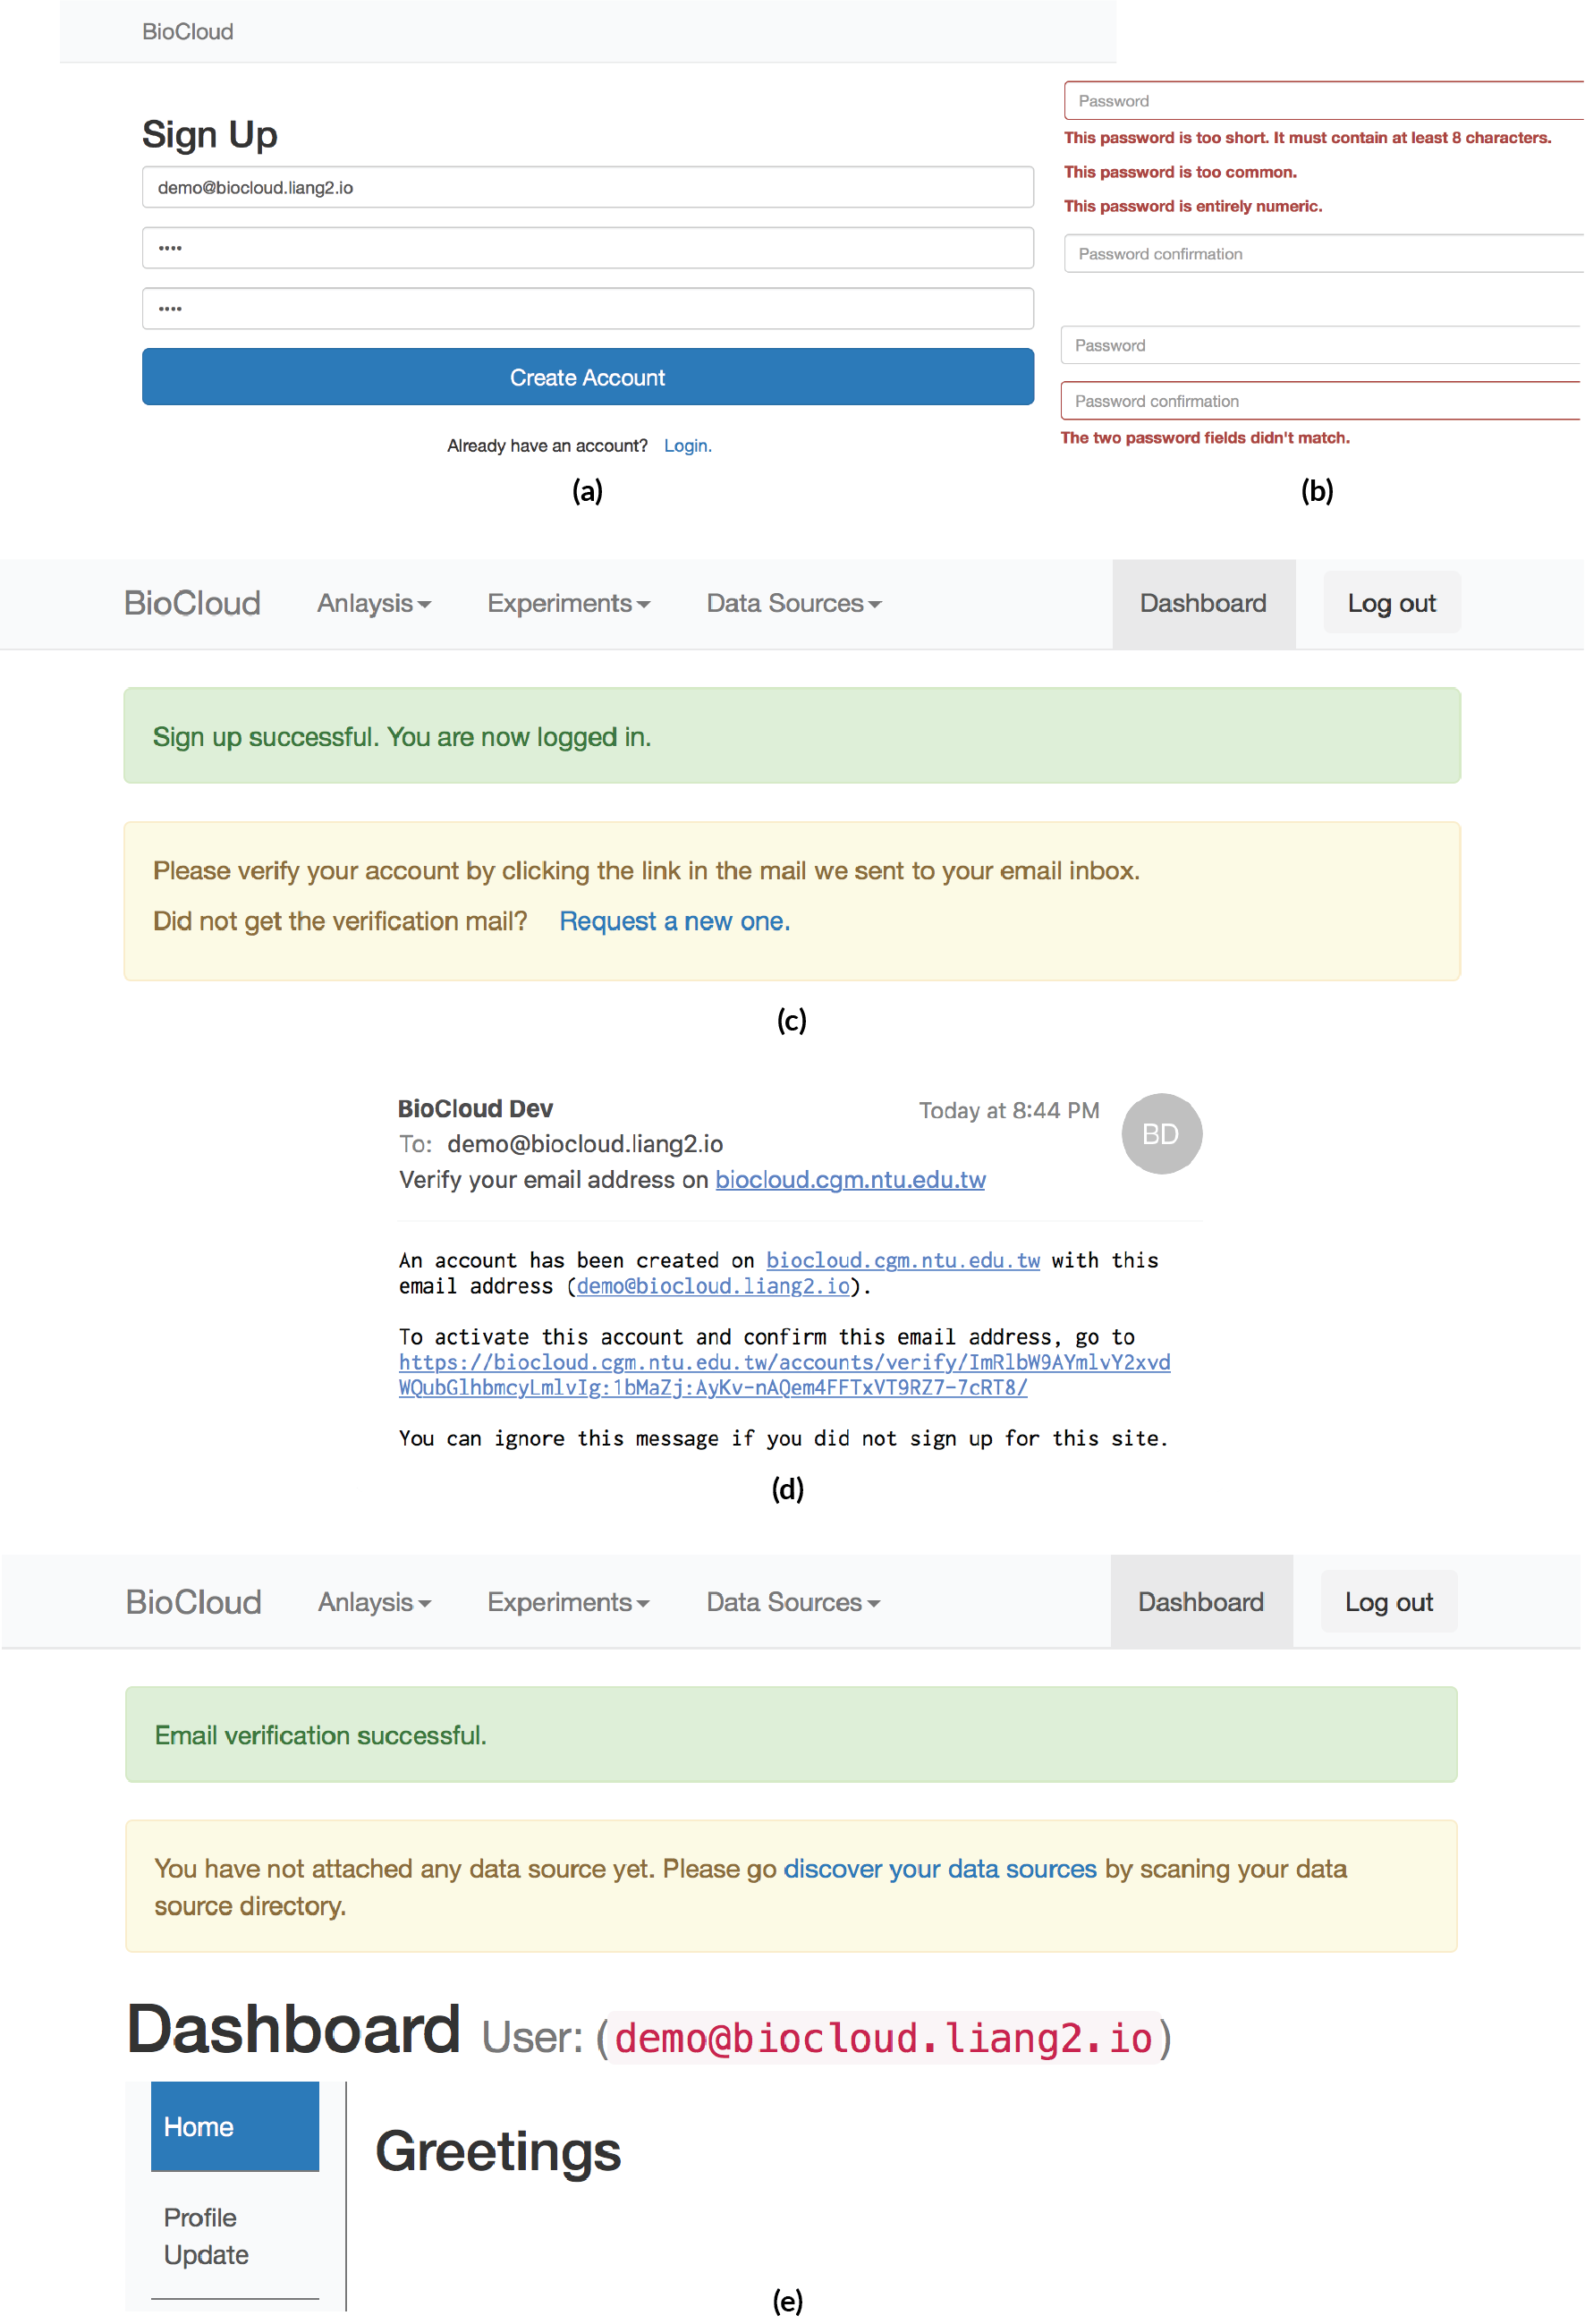
\includegraphics[width=1\textwidth]{images/biocloud_signup}
\caption[Account registration on BioCloud]{
    Account registration on BioCloud.
    (a) Registration form.
    (b) Password validation check.
    (c) Welcome screen after signup with action hint messages.
    (d) Verification email.
    (e) Welcome screen after email verifiction.
}
\label{fig:biocloud-signup}
\end{figure}


A user dashboard is available for user-related settings as shown in
Figure~\ref{fig:biocloud-dashboard}(b). User profile including user name and
authentication number can be updated here. Password can be changed via the link
in the password section in profile update, as shown in
Figure~\ref{fig:biocloud-dashboard}(b). For staff and superuser with special
permission, they can access to the admin interface of BioCloud in user
dashboard via an extra tab ``Admin'', as shown in
Figure~\ref{fig:biocloud-dashboard}(d). Admin interface will be introduced in
Section~\ref{s:biocloud-admin}.

\begin{figure}[!p]
\centering
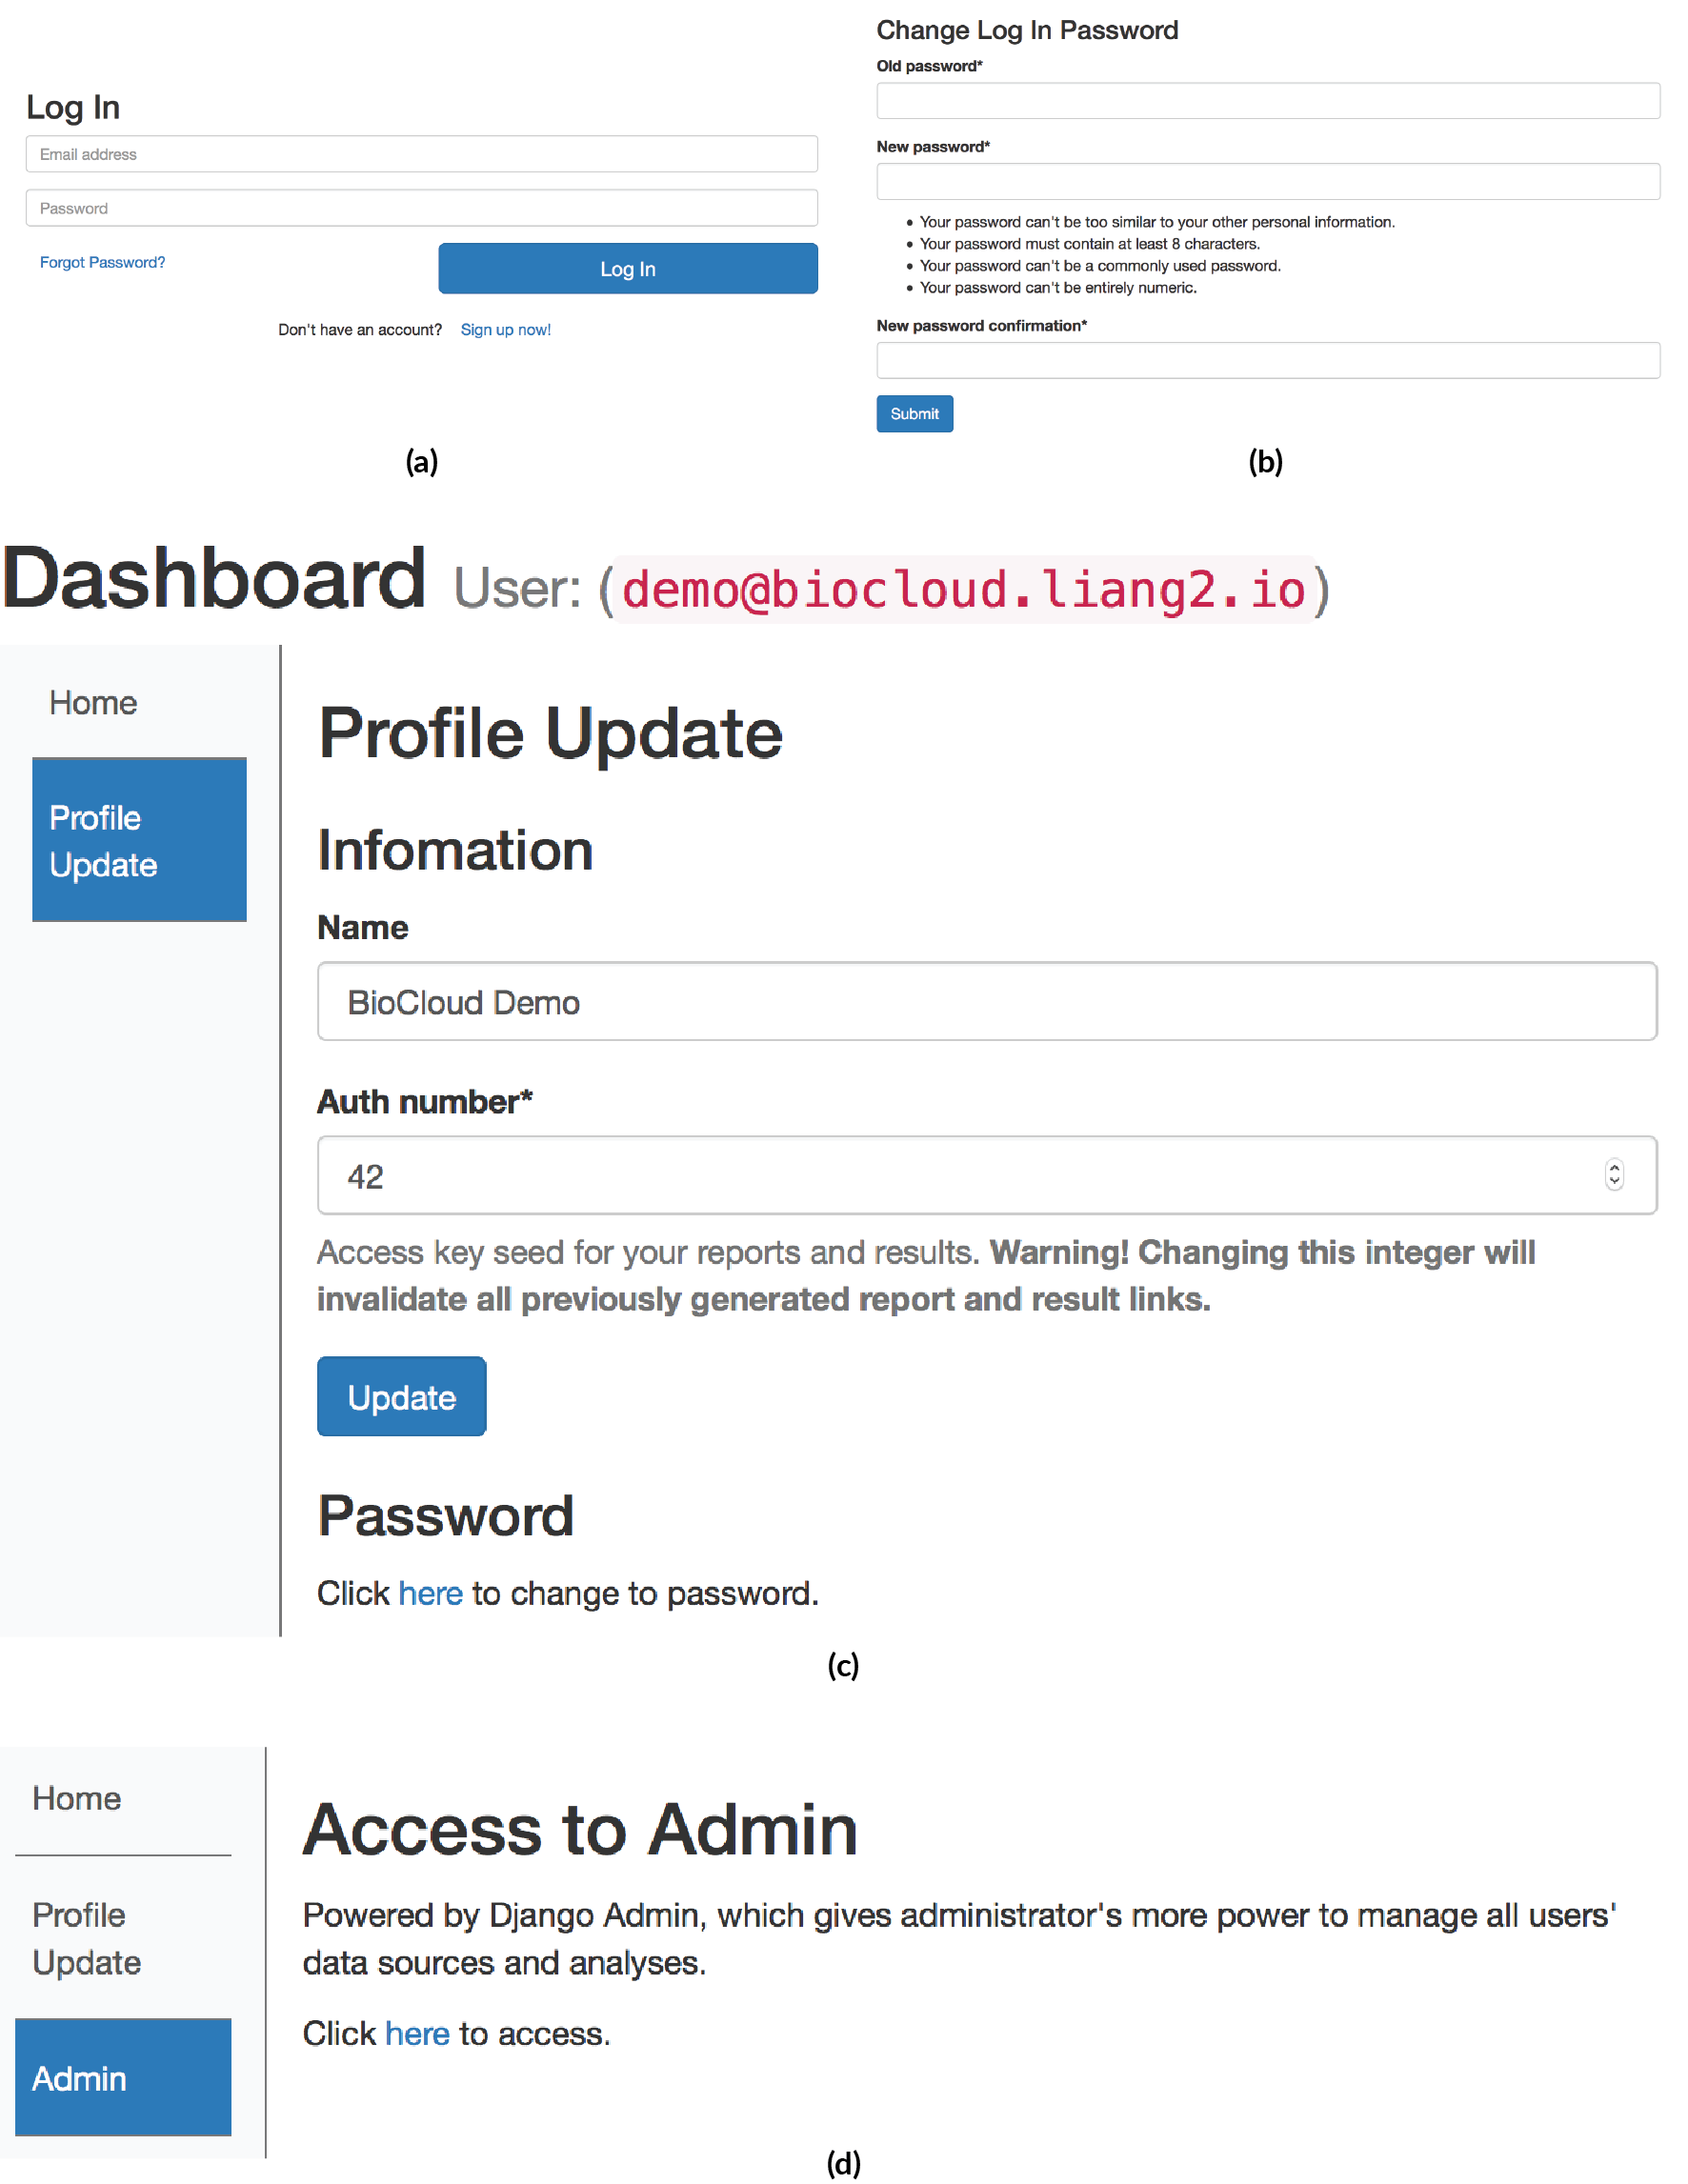
\includegraphics[width=1\textwidth]{images/biocloud_dashboard}
\caption[Login and user dashboard on BioCloud]{
    Login and user dashboard on BioCloud.
    (a) Login form.
    (b) Password change form available through profile update.
    (c) Profile update form.
    (d) For staff and superuser's dashboard, an extra tab to the admin
    interface is shown.
}
\label{fig:biocloud-dashboard}
\end{figure}





\section{Data source discovery}

As a newly registered user, a message was always shown to hint user to attach
their data sources to BioCloud. User can find their specific data source folder
from menu Data Source \textrightarrow List, as shown in
Figure~\ref{fig:biocloud-data-source}(b). For the demo user, location of the
data source folder on BioCloud server was:

\begin{CVerbatim}[fontsize=\small]
/biocloud/data_sources/2/
\end{CVerbatim}

\vspace{-1em}\noindent
Upon new data sources being added, BioCloud updated its database by comparing
the data sources in record with that in current folder. All new discovered data
sources will be listed with guess of sample name and file type, as shown in
Figure~\ref{fig:biocloud-data-source}(a). User can pass the SHA2-256 checksum
value for each file computed locally. BioCloud computed the checksum of these
files and compared the value with that supplied by the user. User can check and
update the detail of their recorded data sources, as shown in
Figure~\ref{fig:biocloud-data-source}(b). BioCloud also guessed the strand for
pair-end FASTA/Q files. The information was recorded at the metadata column in
JSON format.

\begin{figure}[!tbp]
\centering
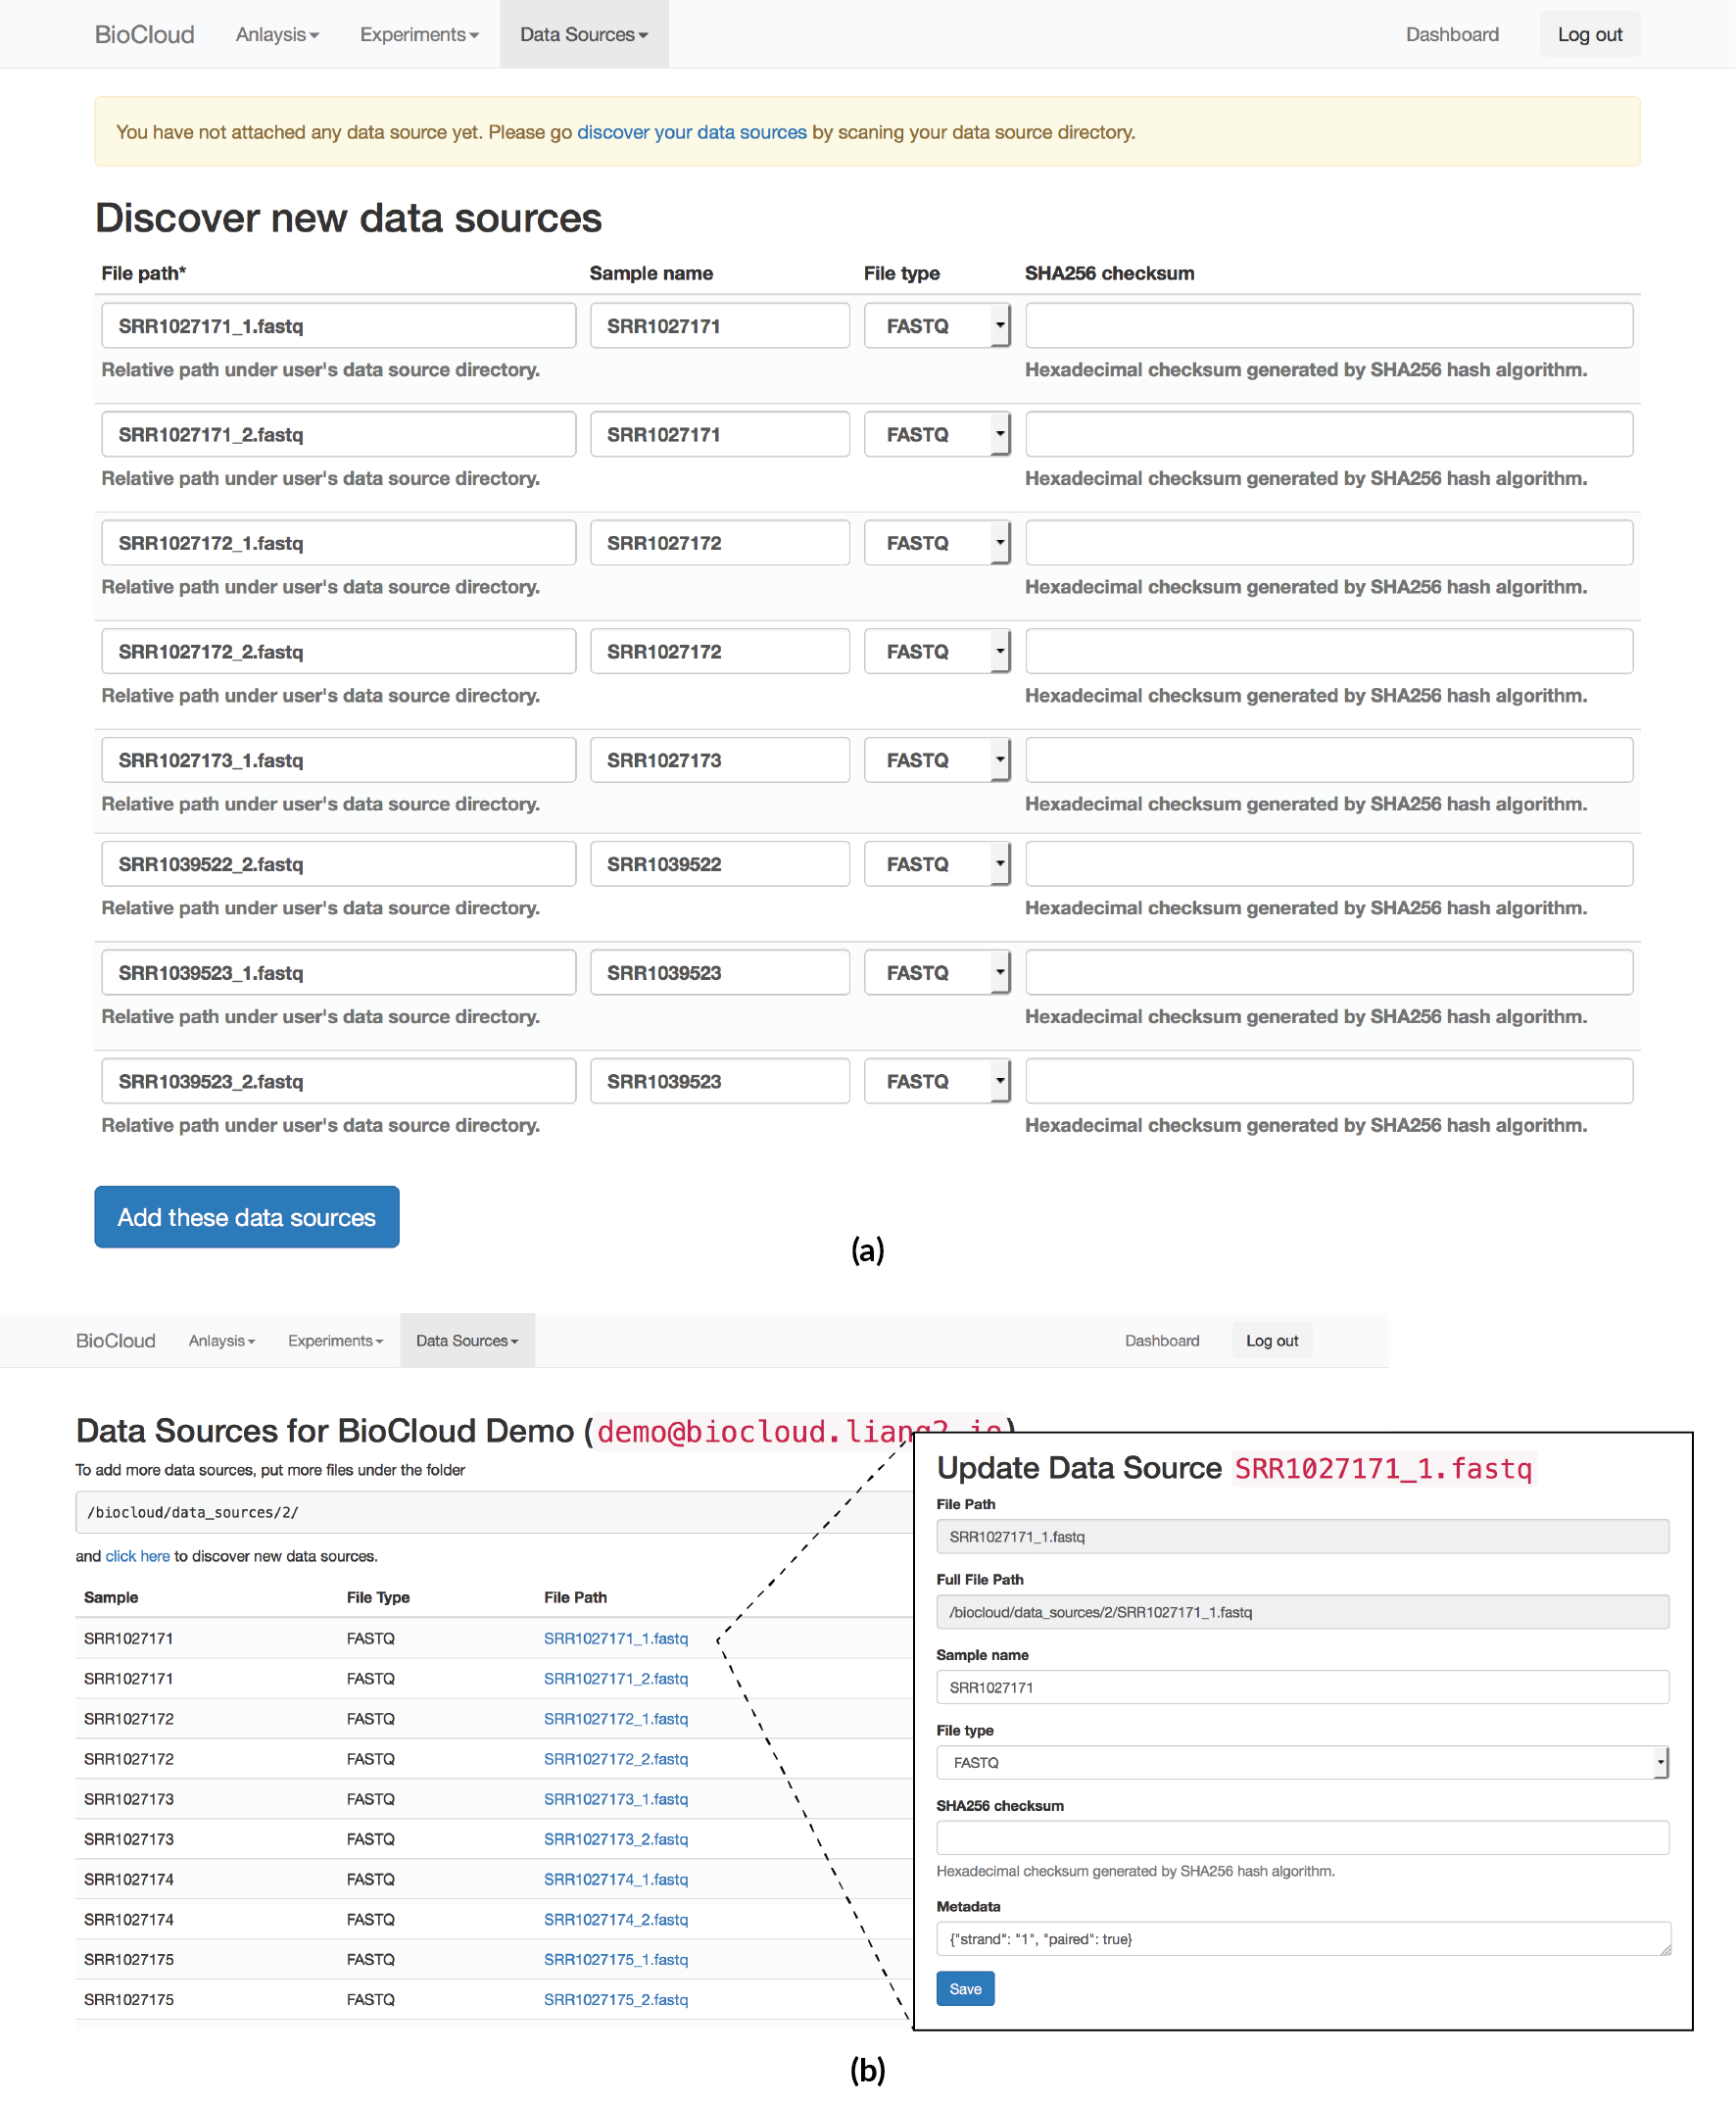
\includegraphics[width=1\textwidth]{images/biocloud_data_source}
\caption[Data source management on BioCloud]{
    Data source management on BioCloud.
    (a) Discovery of new ata sources.
    (b) List and detail view of data sources.
}
\label{fig:biocloud-data-source}
\end{figure}





\section{Experiment design}

\begin{figure}[!tbp]
\centering
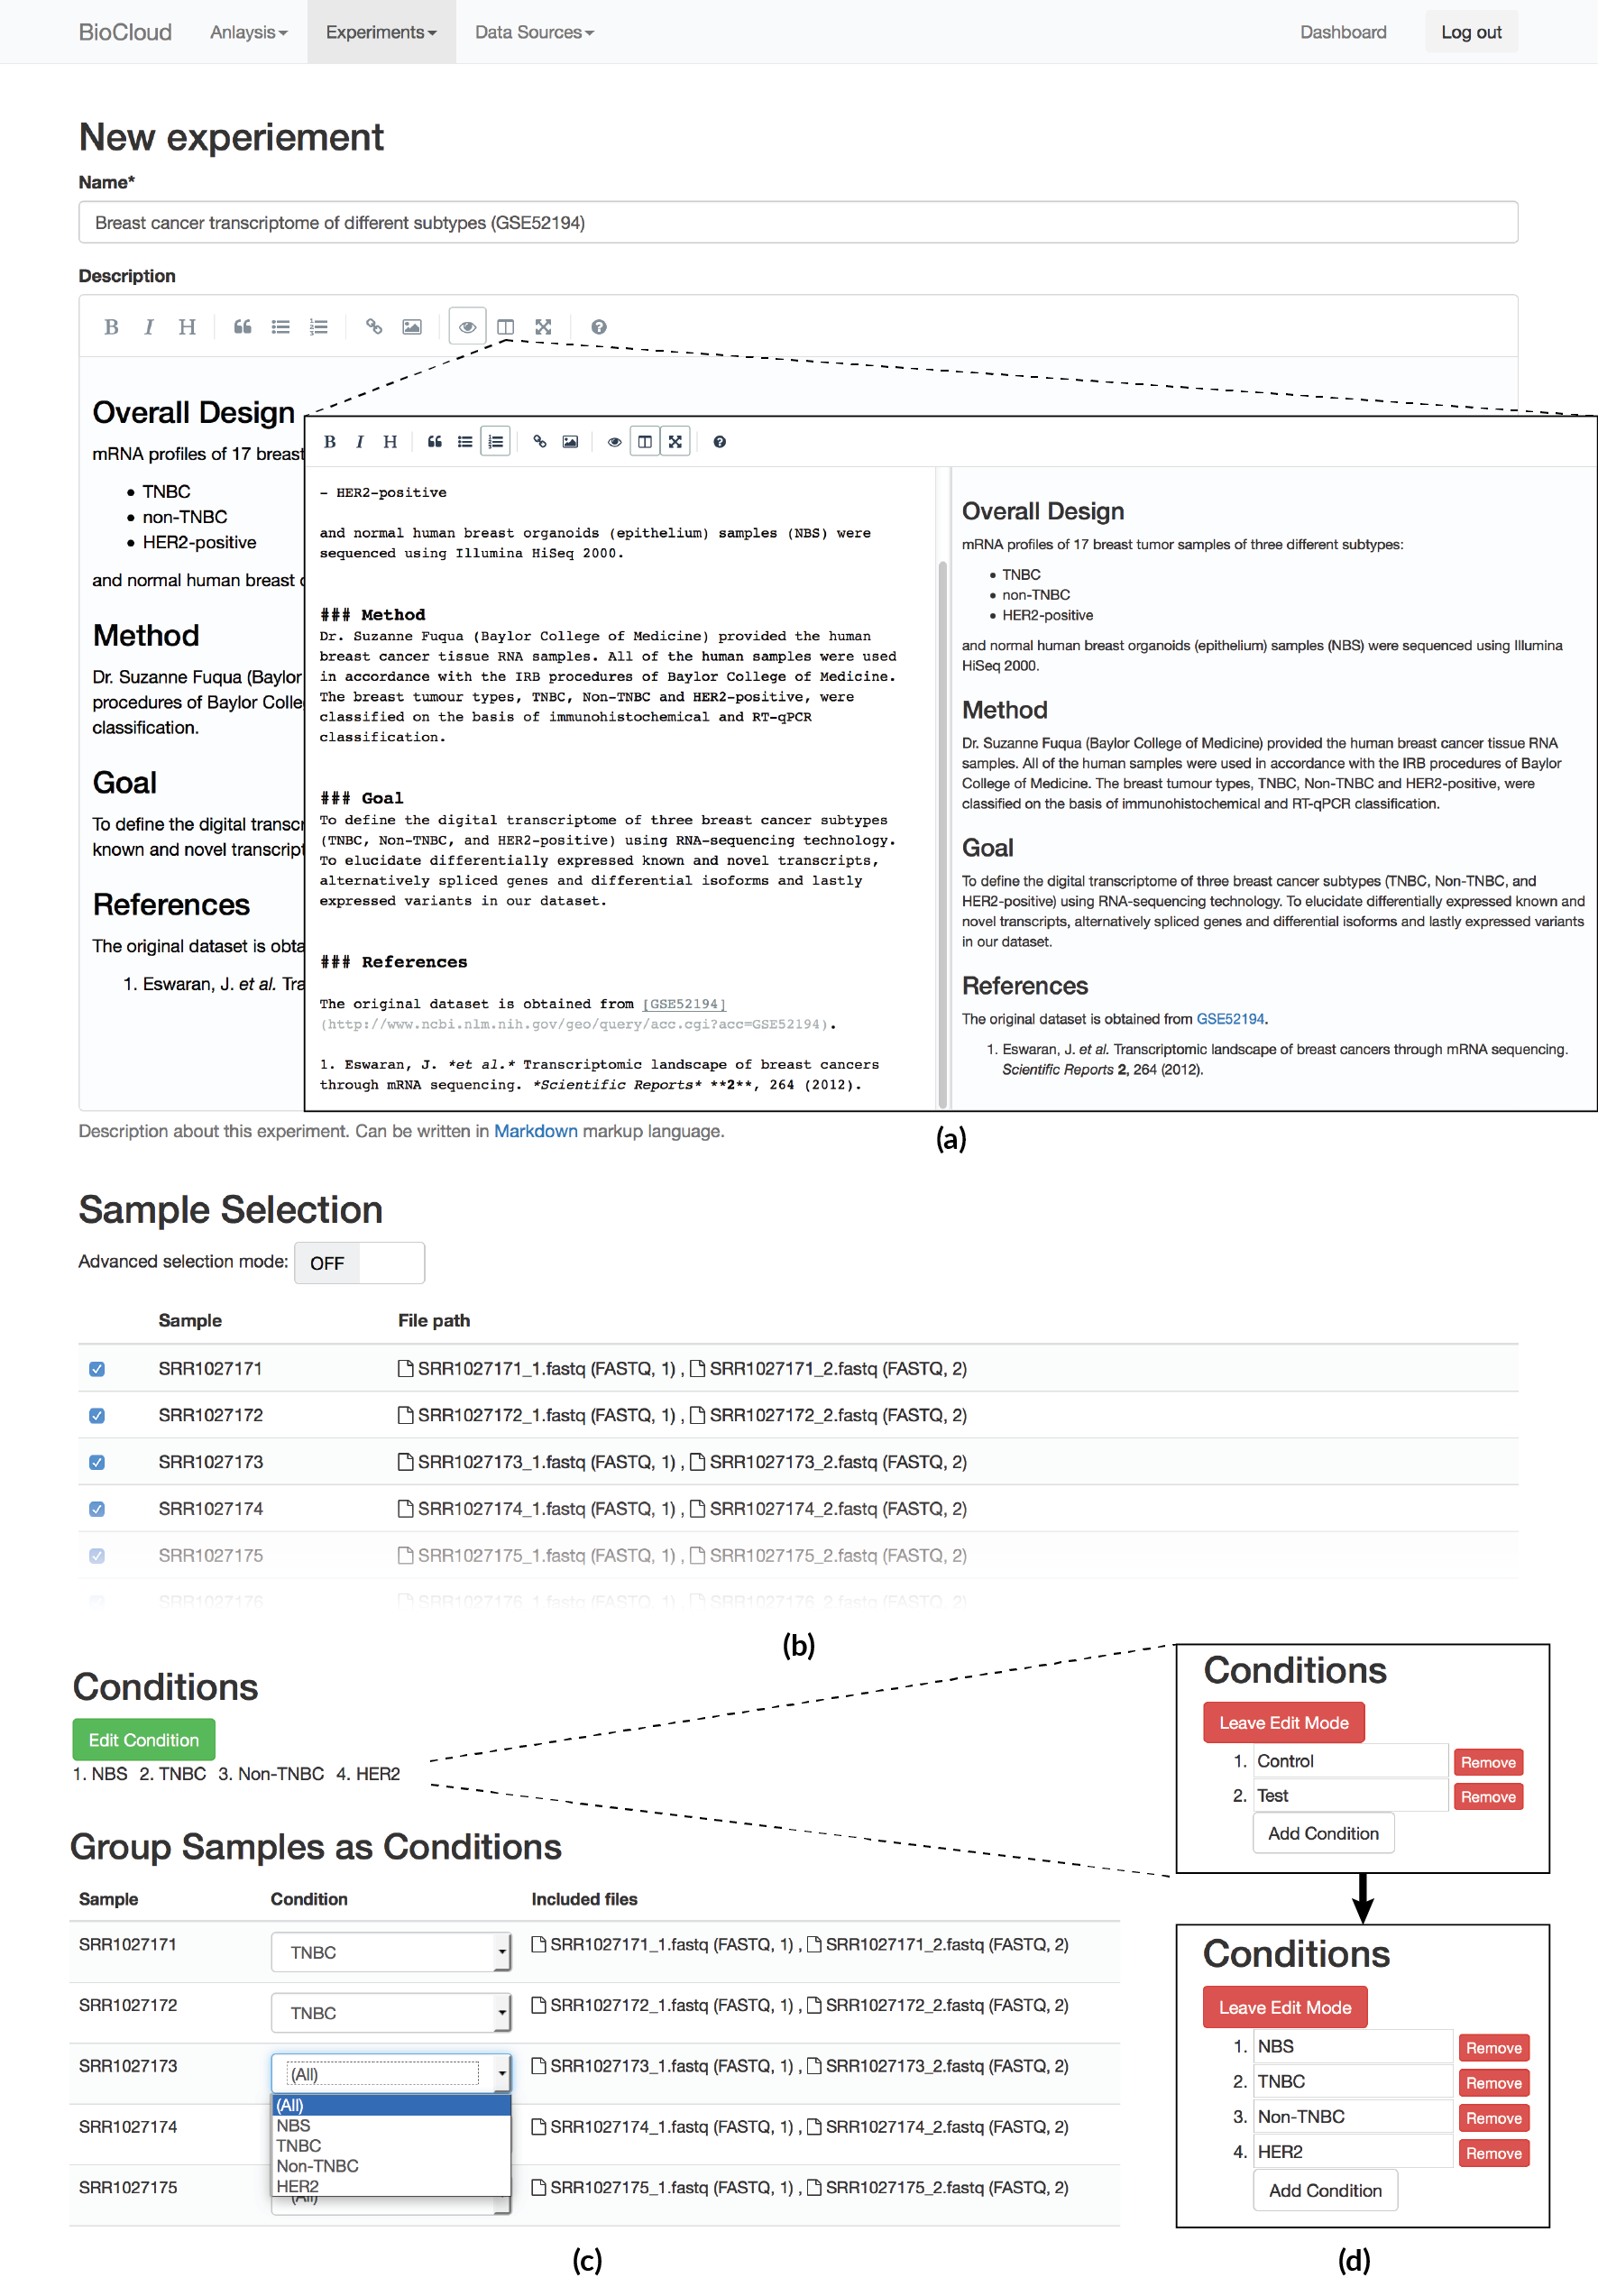
\includegraphics[width=1\textwidth]{images/biocloud_experiment_design}
\caption[Experiment design on BioCloud]{
    Experiment design on BioCloud.
    (a) Description Markdown editor in full screen.
    (b) Upper half of the experiment design form.
    (c) Condition assignment of samples.
    (d) Condition design.
}
\label{fig:biocloud-experiment-design}
\end{figure}

\begin{figure}[!tbp]
\centering
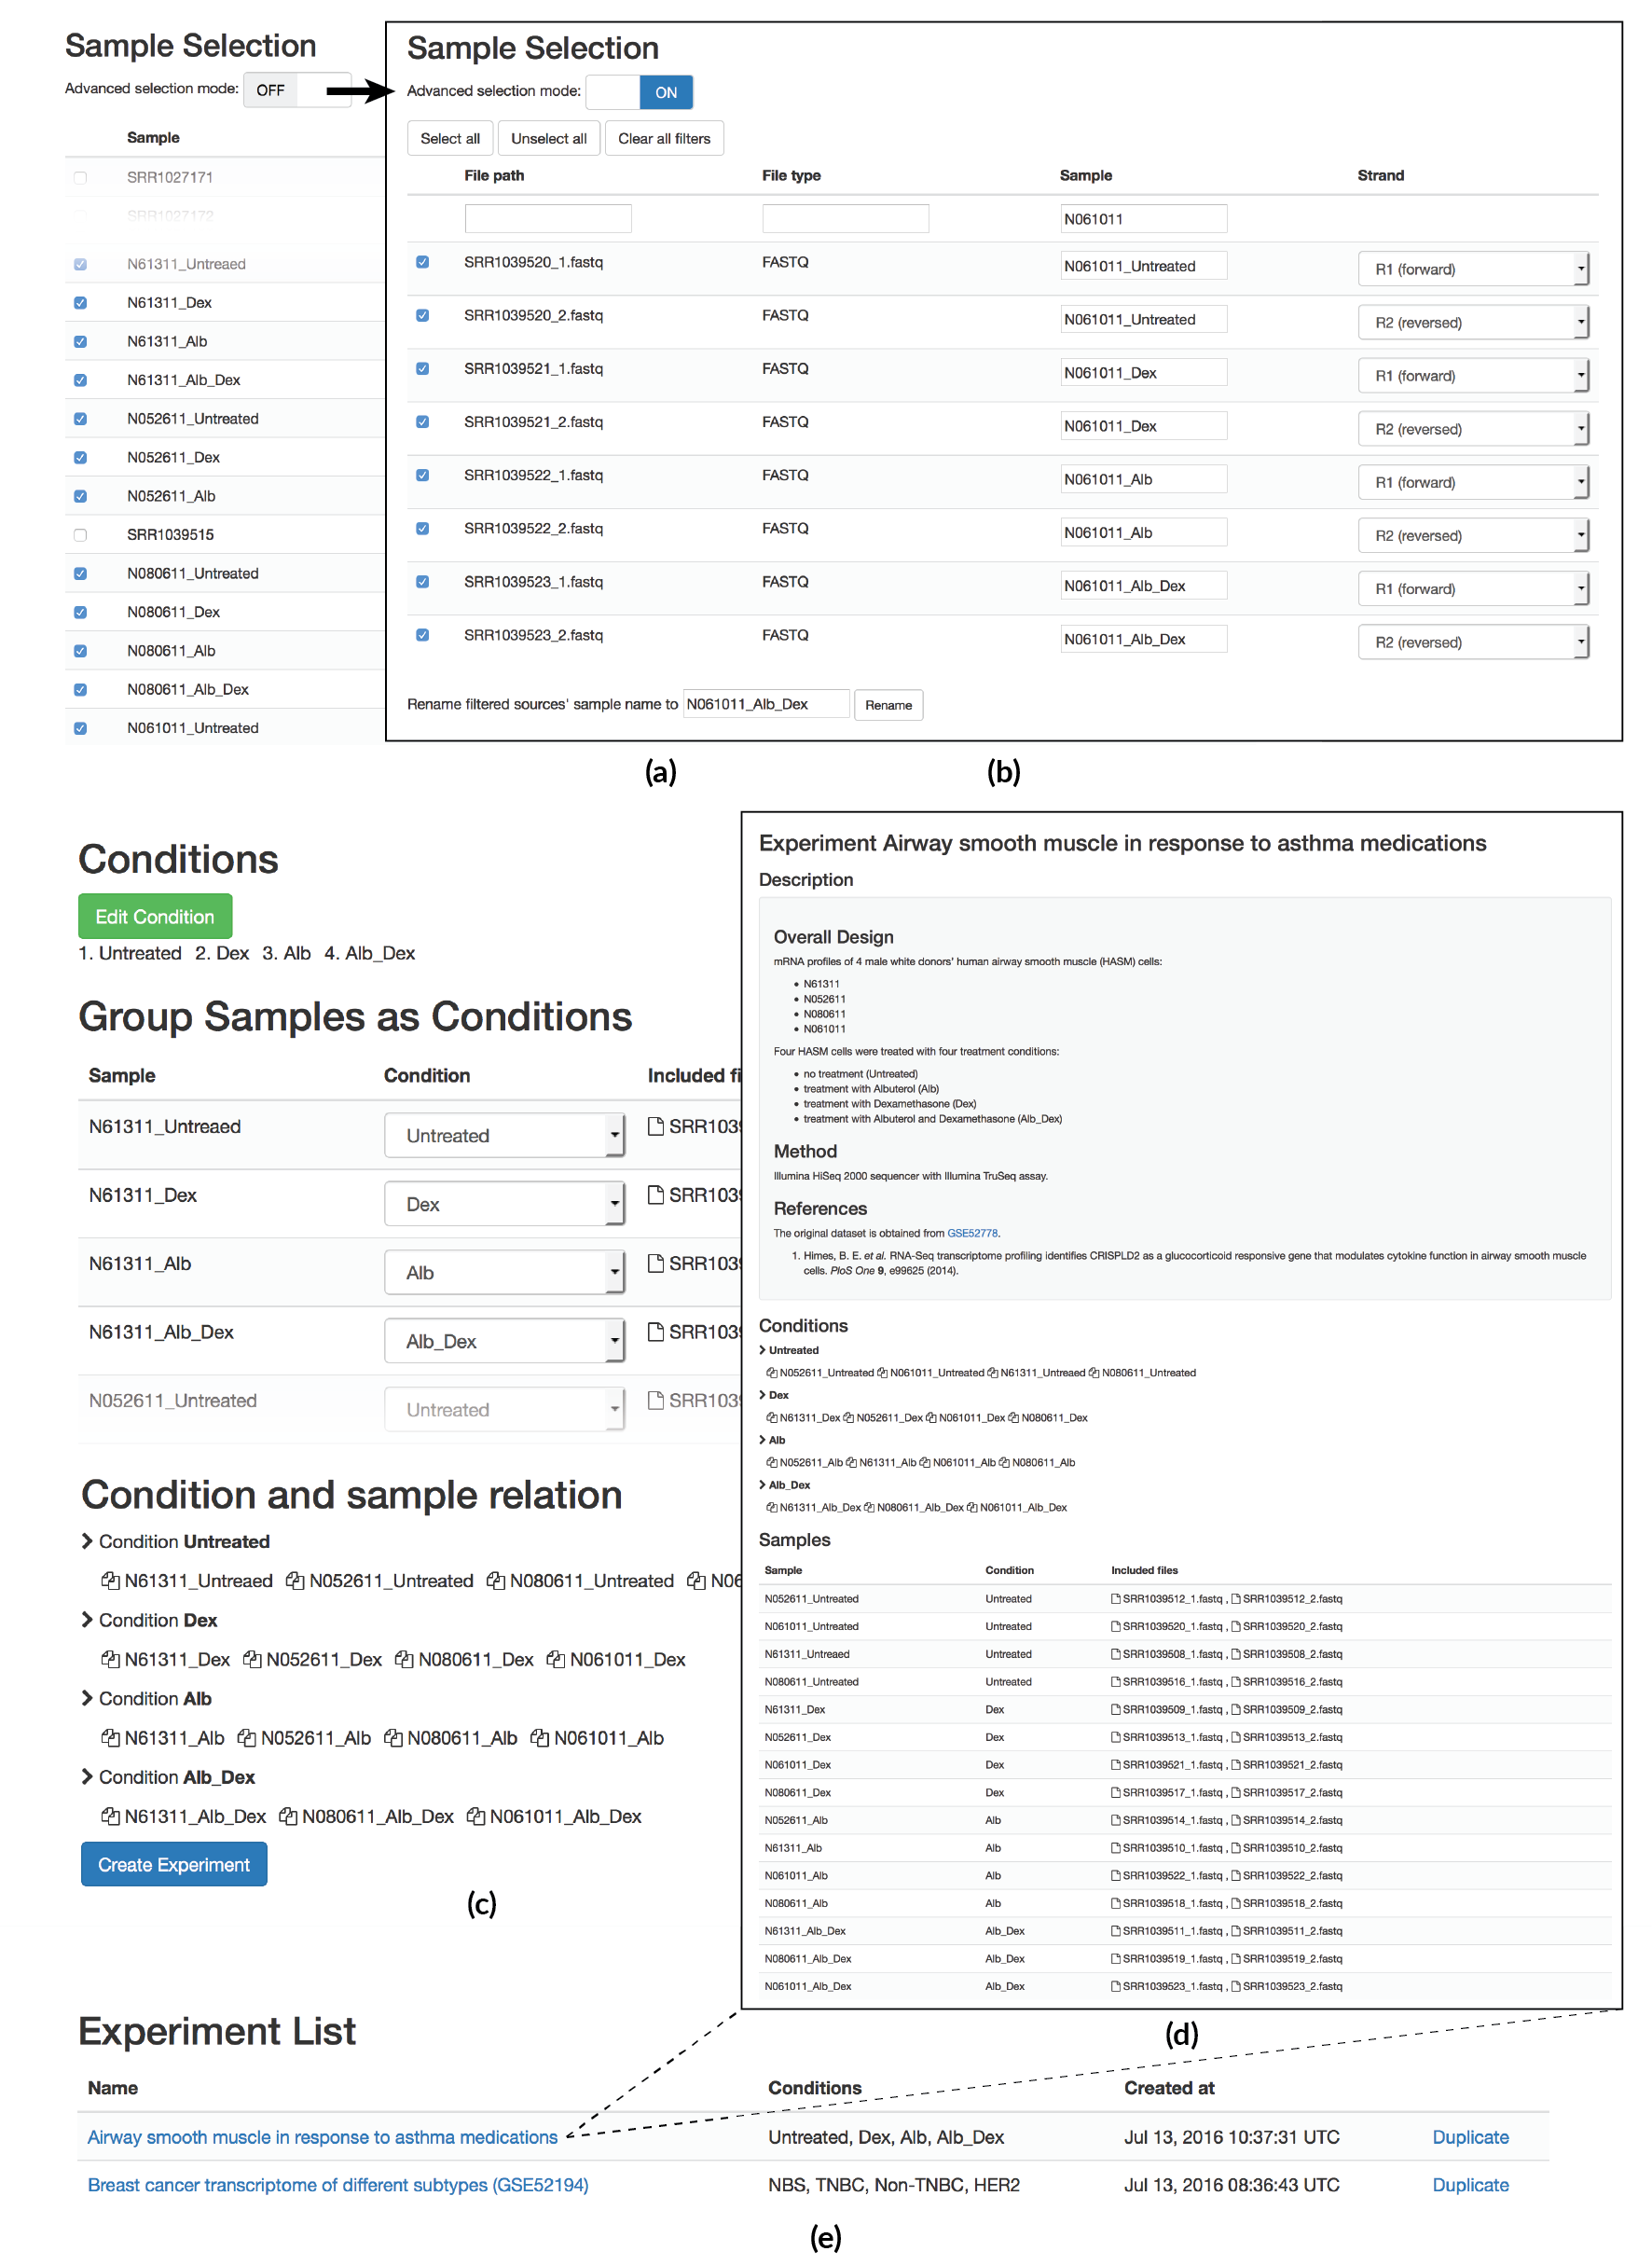
\includegraphics[width=1\textwidth]{images/biocloud_experiment_sample_condition}
\caption[Experiment design on BioCloud (cont'd)]{
    Experiment design on BioCloud (cont'd).
    (a)
    (b)
    (c)
    (d)
    (e)
}
\label{fig:biocloud-experiment-design}
\end{figure}



% general description
Experiment design groups selected samples into user defined conditions to
represent the biological experiment design. BioCloud will warn the user if one
try to create experiment without adding any data source. All experiment related
functions are under the menu item ``Experiment''. Here the demo user added all
datasets mentioned in Section~\ref{s:dataset}. When the user created a new
experiment, one was guided to fill in experiment description, select data
sources, create conditions, assign conditions step by step, as shown in
Figure~\ref{fig:biocloud-experiment-design}. User first filled in the
experiment name and description. Experiment description was written using the
Markdown syntax and an editor based on SimpleMDE was provided, as shown in
Figure~\ref{fig:biocloud-experiment-design}(a). Headings, enumerated lists, and
hyperlinks can be created to help user collect all the related information. The
rendered description can be live previewed in full screen side-by-side mode.

% sample selection
To actually construct the experiment design, user first started with sample
selection, as shown in Figure~\ref{fig:biocloud-experiment-design}(b). By
default the simple mode of selection sample was shown, where data sources of
same sample names were selected together and the default sample name was used.
Selected samples were simultaneously shown in the condition design section
below (Figure~\ref{fig:biocloud-experiment-design}(c)) with the help of
reactive programming. All the elements in the experiment design form shares the
same underlying data structure. Therefore, as a sample was selected, all its
data sources are marked as selected and Vue.js updated all the DOMs that
depended on the selected data sources.

% simple and advanced mode
An advanced mode of selection mode was provided so user can have detail control
on the inclusion of samples, as shown in
Figure~\ref{fig:biocloud-experiment-sample-condition}(b). When it is enabled
data sources were listed one by one and their sample names become modifiable.
User can select one strand of a pair-end sample, or override the existed sample
name of data sources. Data sources can be filtered based on file name, file
type, and sample name.

% condition
By default samples are of condition ``(All)'', a special condition implying the
sample does not belong to any given condition. Currently no pipeline requires
the special condition but it is implemented so custom pipeline can let user
specify experiment-wise input. By default there were two conditions: Control
and Testing. User can remove, edit, and add conditions, as shown in
Figure~\ref{fig:biocloud-experiment-design}(d). They were dynamically rendered
as available options of selected sample's conditions, as shown in
Figure~\ref{fig:biocloud-experiment-design}(e). Note that it is considered safe
and there will be no data loss if user later modifies the condition name.
Order of conditions was kept in the database. In analysis, condition specified
later was compared with those specified earlier for each condition pair.
Generally, one should put control or normal condition as the first condition.
In the figure, breast cancer dataset defined conditions: NBS, TNBC, Non-TNBC,
HER2 in order, where NBS was the normal condition of the dataset. As user was
designing the conditions, a preview of the current experiment was displayed in
the last section, as shown in
Figure~\ref{fig:biocloud-experiment-sample-condition}(c).

%experiment list
User can view one's submitted experiments at the experiment list view, as shown
in Figure~\ref{fig:biocloud-experiment-sample-condition}(e). Detail of the
experiment can be found by clicking the link of each experiment in the
experiment list view, as shown in
Figure~\ref{fig:biocloud-experiment-sample-condition}(d). Users are not allowed
to modify the experiment conditions, otherwise existed analyses would have
uncertain experiment design. However, one can build a new experiment based on
an existed experiment design.



\section{Analysis design}

\begin{figure}[!p]
\centering
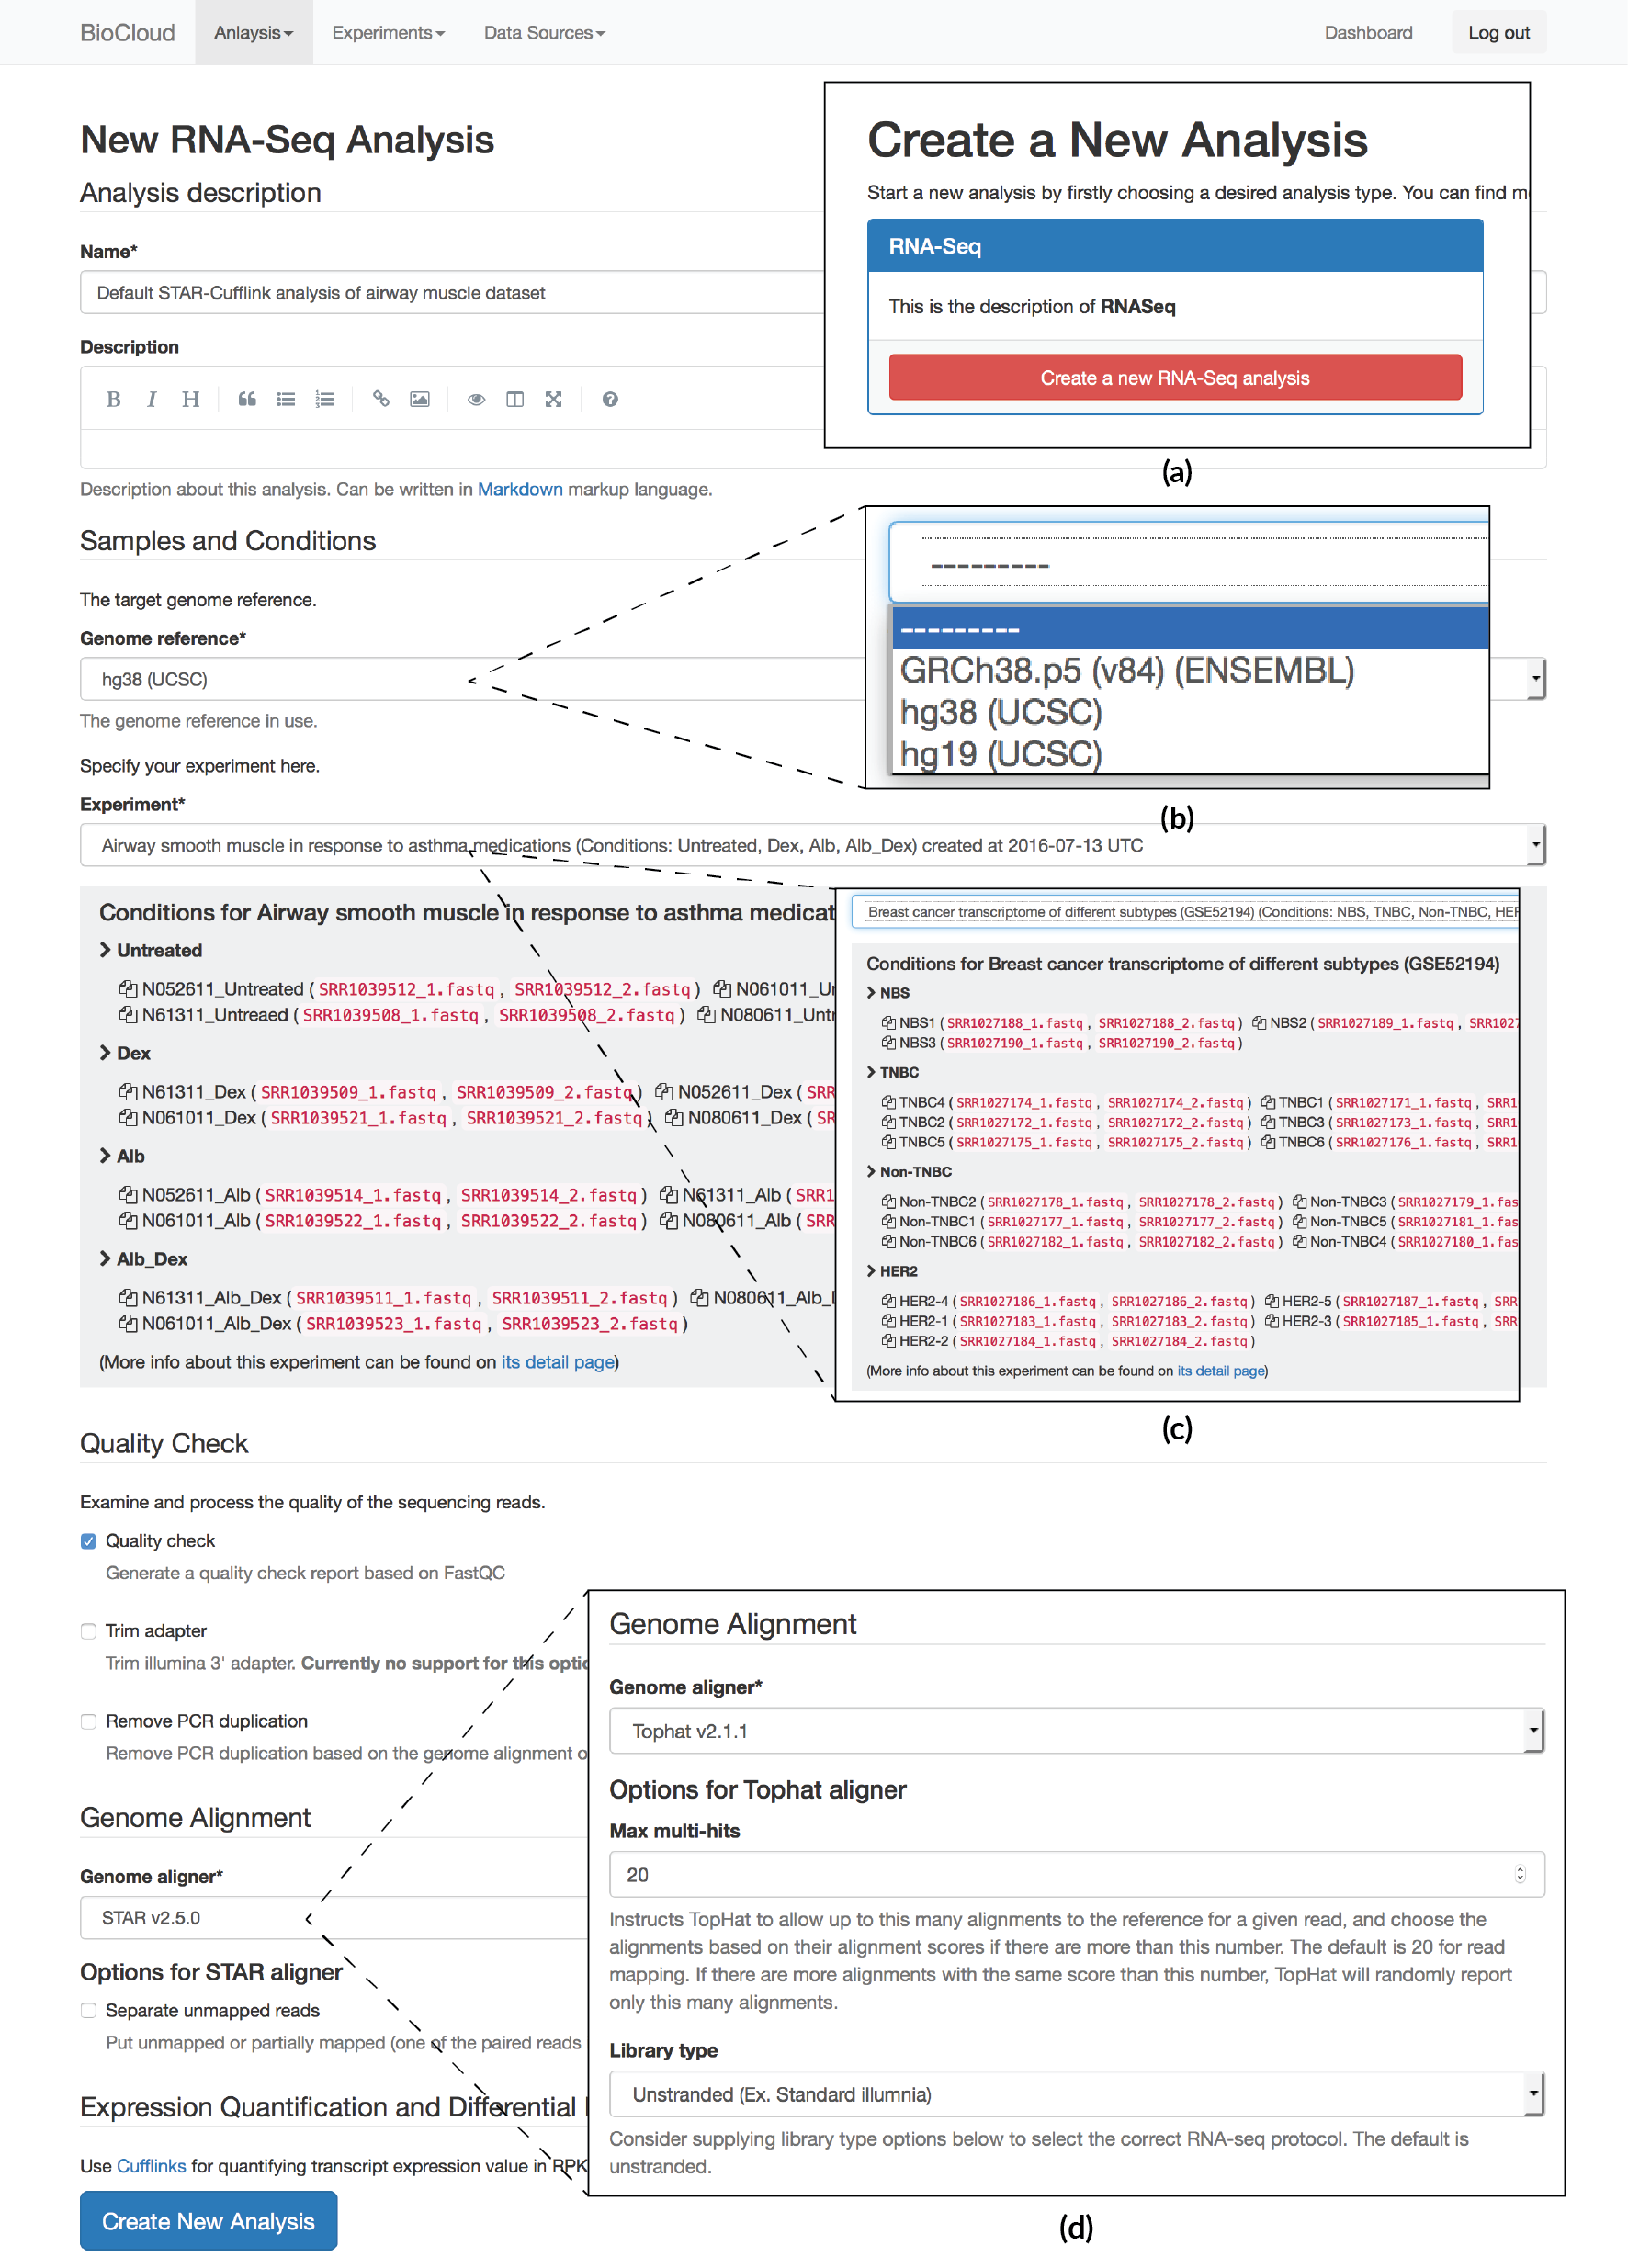
\includegraphics[width=1\textwidth]{images/biocloud_analysis_design}
\caption[Analysis design on BioCloud]{
    Analysis design on BioCloud.
}
\label{fig:biocloud-analysis-design}
\end{figure}



Analysis binds an experiment design and executes one of the available pipelines
with given genome reference and parameters. First user chose the pipeline to
execute, as shown in Figure~\ref{fig:biocloud-analysis-design}(a). It was a
portal which gathered all currently available pipelines defined in the BioCloud
source code. In Figure~\ref{fig:biocloud-analysis-design}, the demo user
selected the Cufflink-based RNA-Seq pipeline. User was then guided to a new
dedicated page for the selected analysis design form. Similar to experiment
design, user can specify name and description in Markdown syntax for the
new analysis.

Some parts of the analysis design form were the same for all analysis
pipelines. All analysis pipelines require genome reference and experiment
design as input. Available genome references were defined by staff or superuser
via the BioCloud admin interface, whose name and provider combined as the
option name as shown in Figure~\ref{fig:biocloud-analysis-design}(b). Here the
human genome reference hg38 provided by UCSC was chosen. User continued to
select the experiment design in use. User can select by the name of one's own
experiment designs, whose conditions and samples will be dynamically rendered
once user made a choice, as shown in
Figure~\ref{fig:biocloud-analysis-design}(c). A link to the experiment detail
view was also provided for more information. Here the human airway smooth
muscle dataset was used.

Finally, rest of the analysis design form was specially defined for
Cufflink-based RNA-Seq pipeline. As described in
Section~\ref{s:rnaseq-pipeline}, there are three available genome aligners in
this pipeline. Each of the aligner has different option sets. Therefore, as
user selected one aligner, only the corresponding options were shown. For
example, in Figure~\ref{fig:biocloud-analysis-design}(d), user changed the
aligner from STAR to Tophat2 and different options were displayed.



\section{Job queue monitoring}

\begin{figure}[!p]
\centering
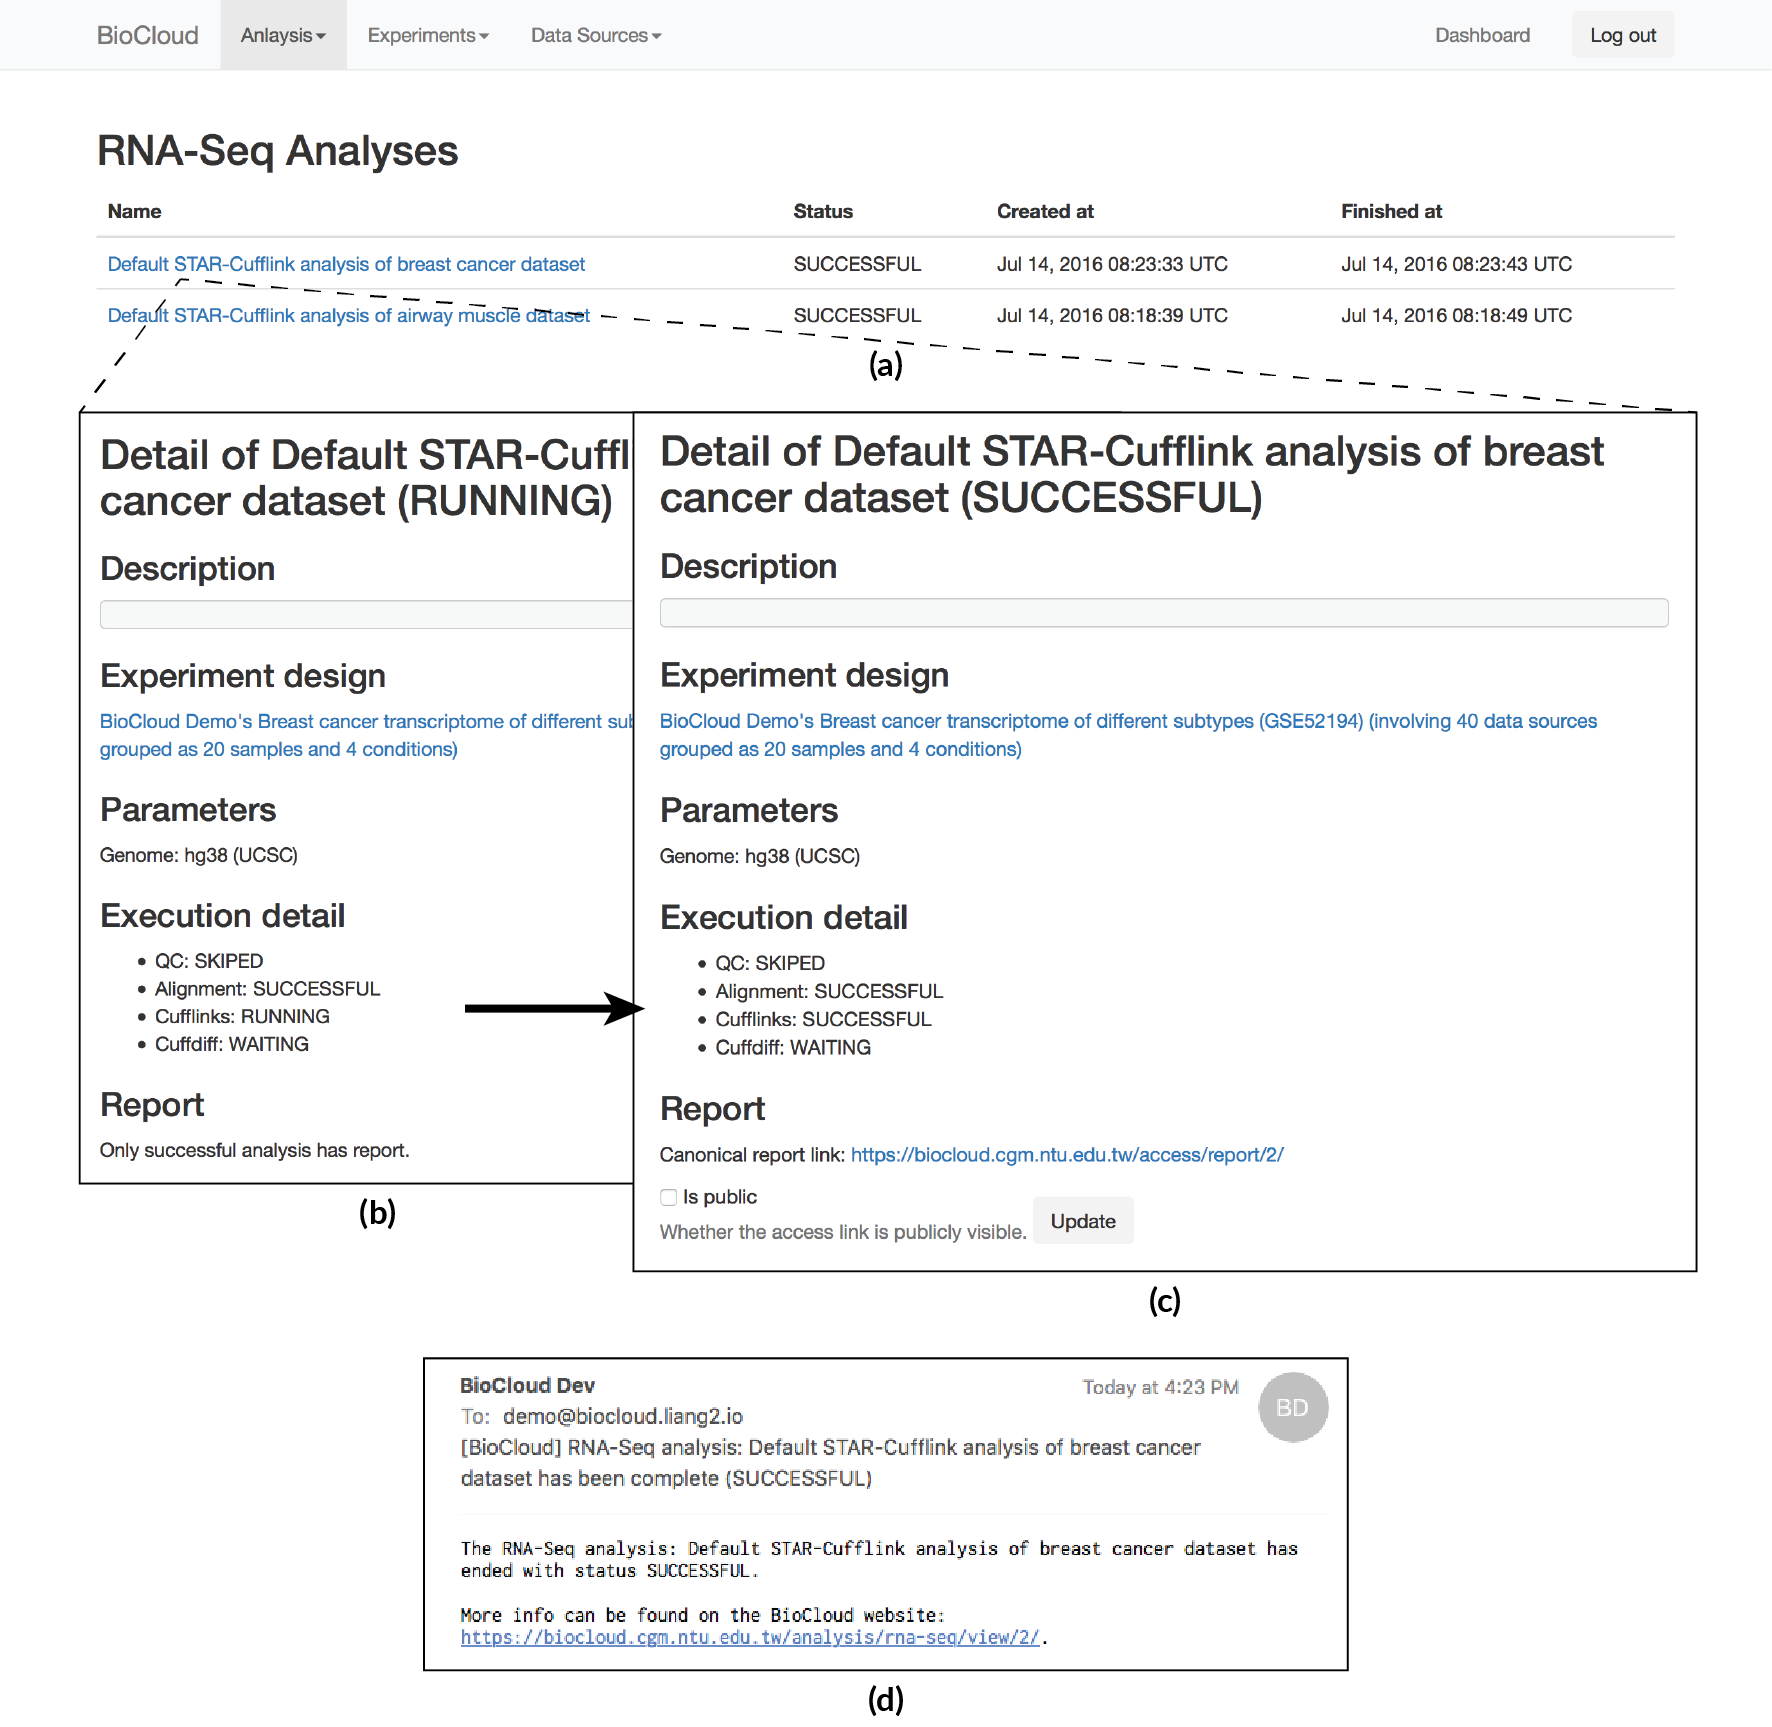
\includegraphics[width=1\textwidth]{images/biocloud_job_monitor}
\caption[Job monitoring on BioCloud]{
    Job monitoring on BioCloud.
}
\label{fig:biocloud-job-monitor}
\end{figure}



% analysis list
% execution detail
% report link and options
% email notification

User could find all executed, queuing and currently running analyses at one's
analysis list view, as shown in Figure~\ref{fig:biocloud-job-monitor}(a). By
clicking on the name of the analysis, user was guided to its detail page. If
the analysis is currently running, its detail will be live updated to reflect
the current status of its execution stages. Some of the stages may be marked as
skipped if user opted out their execution during analysis design. For example,
Figure~\ref{fig:biocloud-job-monitor}(b) shows an analysis currently running
the Cufflinks stage. QC stage was skipped thus this analysis did not perform
the quality check. Stages behind the currently running stage, e.g. Cuffdiff
stage in the figure, were marked as waiting.

As the analysis execution ended, user was notified by mail with the link to the
analysis detail page, as shown in Figure~\ref{fig:biocloud-job-monitor}(d). If
the analysis execution was successful, the summary report was generated and its
link would be shown in its analysis detail page.
Figure~\ref{fig:biocloud-job-monitor}(c) showed the successful execution of the
analysis described above. Summary report was generated and its canonical link
was given below the execution detail. When user clicked on the link, one would
be redirect to the report link with HMAC-based access token. During logged in,
both links will maintain valid until user modifies one's authentication number
at the user profile page, which invalidate the current HMAC-based access token
while the canonical link will always be accessible. By default, all reports and
results were restricted to private access only. User can opt the current
analysis to be public by changing the ``is public'' setting shown in
Figure~\ref{fig:biocloud-job-monitor}(c).



\section{Admin interface}
\label{s:biocloud-admin}

\begin{figure}[!p]
\centering
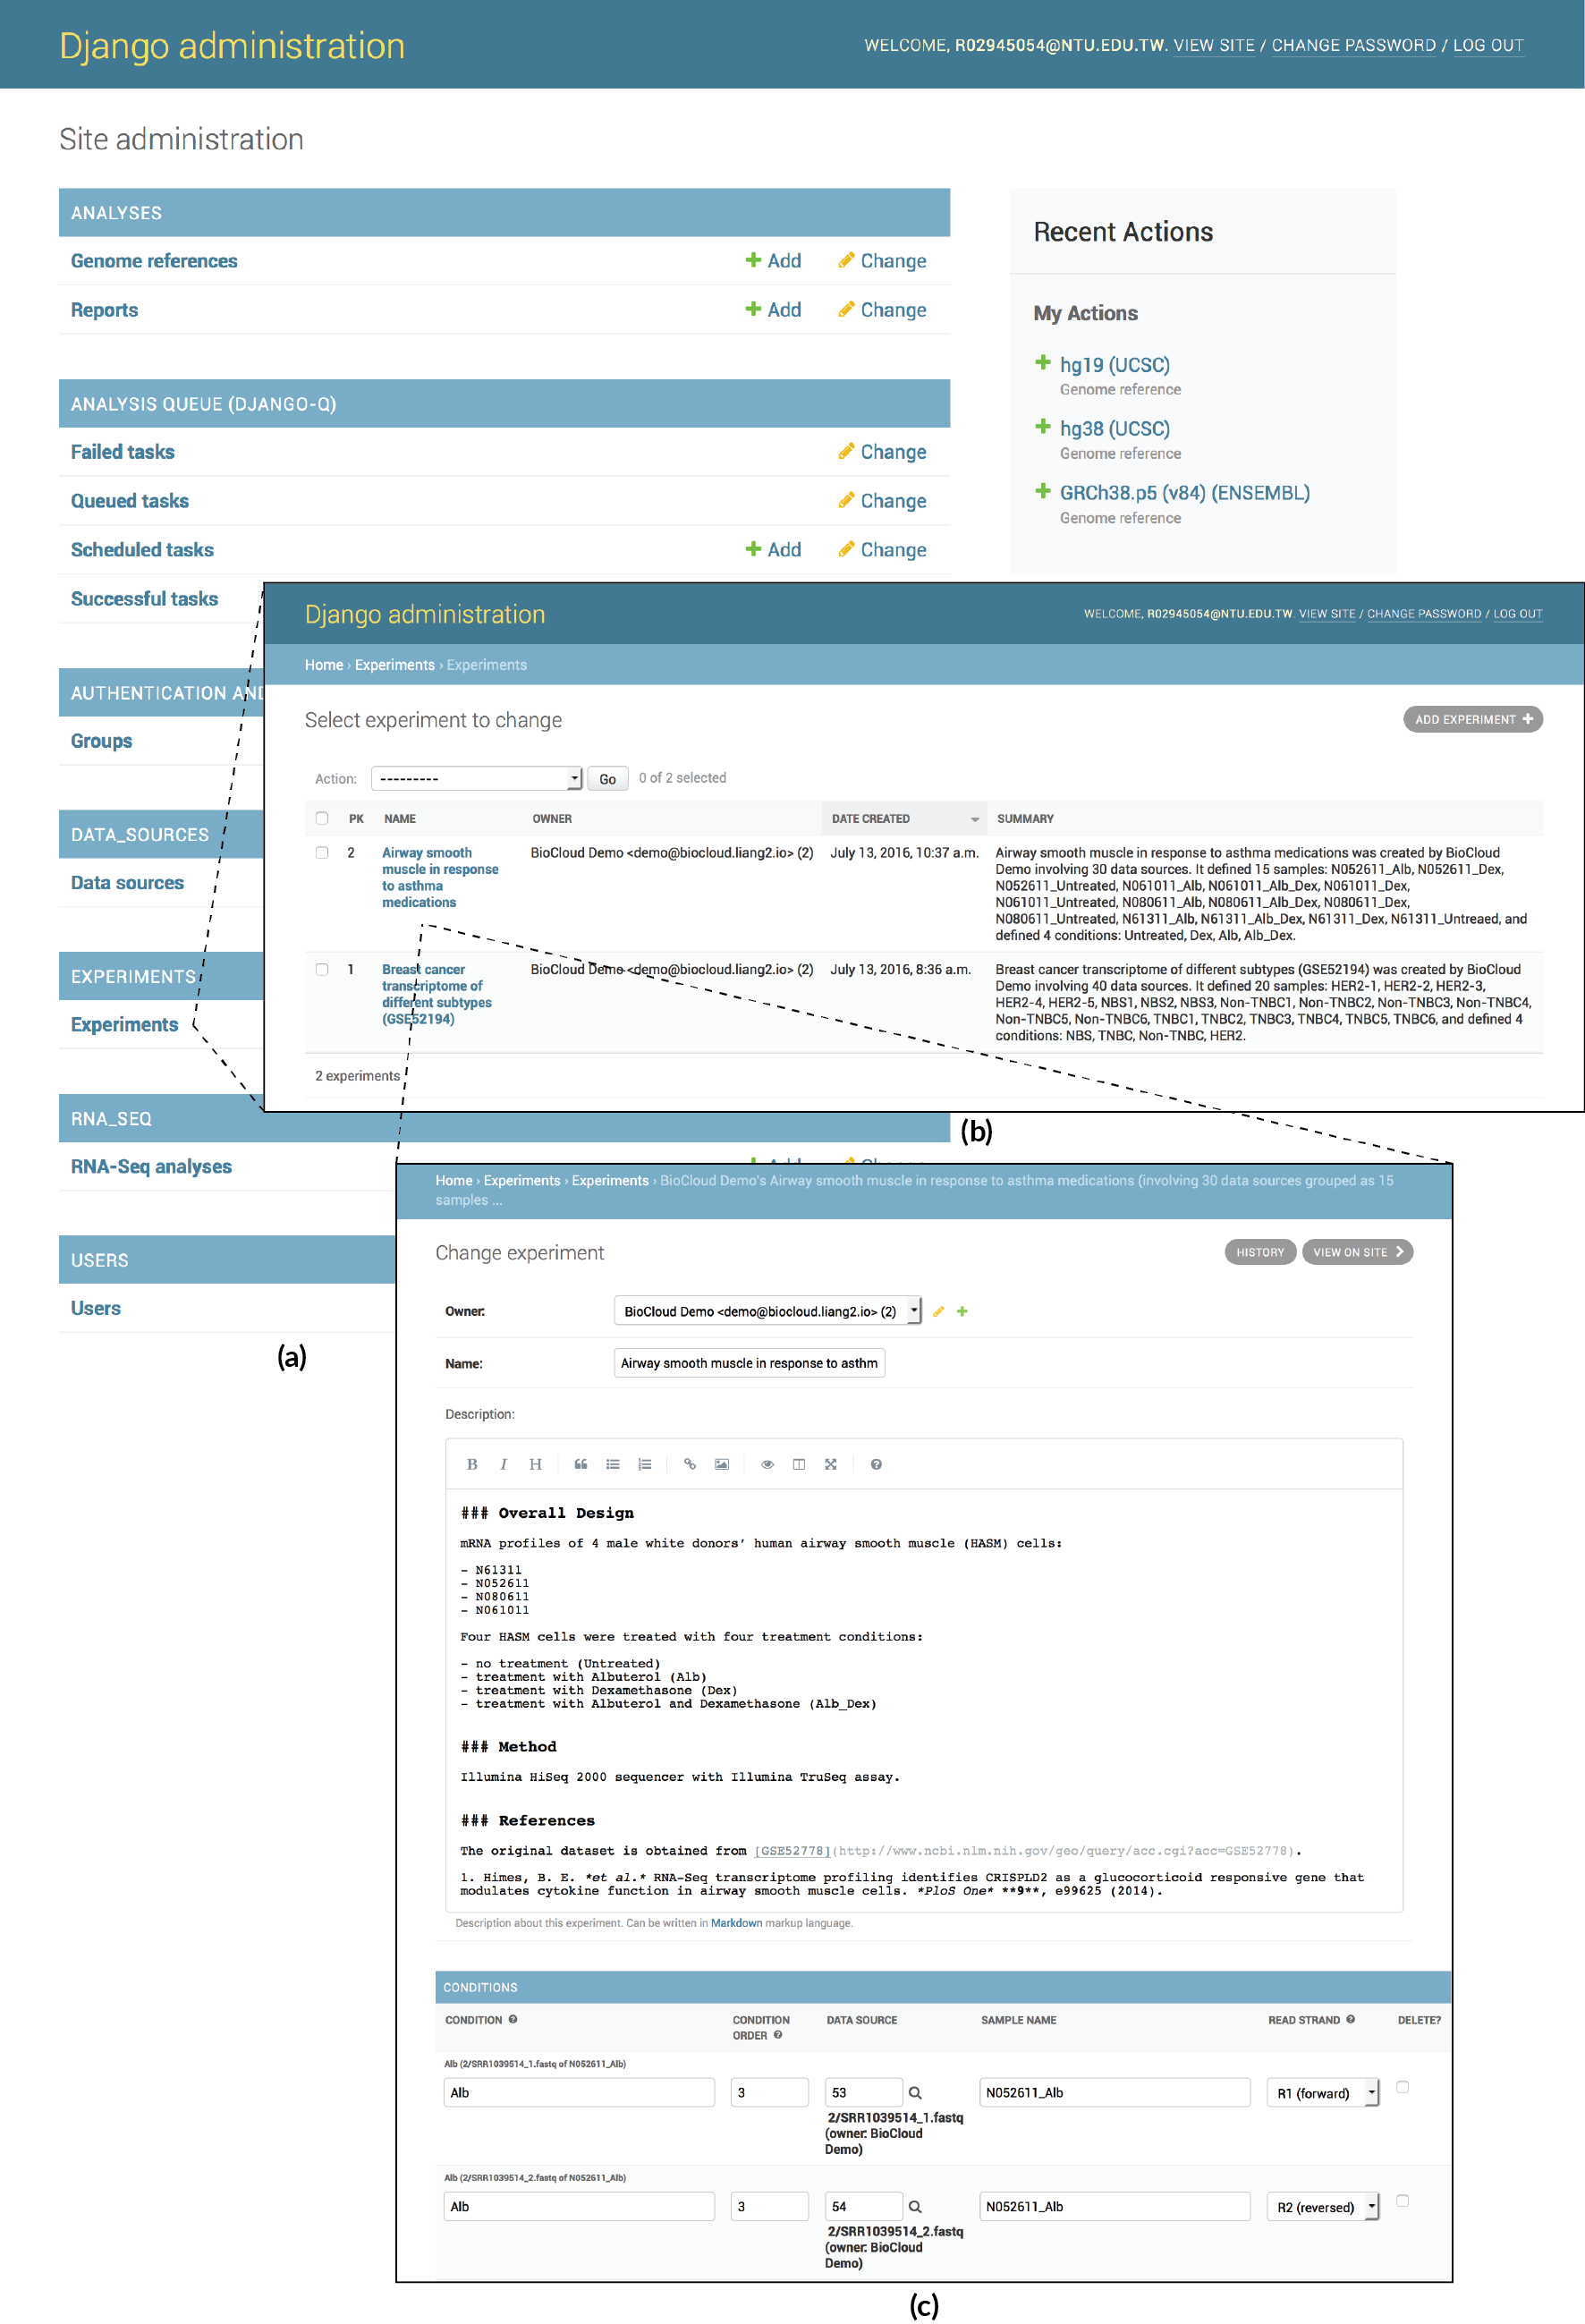
\includegraphics[width=1\textwidth]{images/biocloud_admin}
\caption[Admin interface of BioCloud]{
    Admin interface of BioCloud.
}
\label{fig:biocloud-admin}
\end{figure}




Before moving on to the summary report of the analysis, since most of the
BioCloud's functions have been covered, we can now look at its admin interface.
As shown in Figure~\ref{fig:biocloud-dashboard}(d), staff and superuser will
have the special permission to access the admin interface of BioCloud. The
homepage of the BioCloud admin is shown in Figure~\ref{fig:biocloud-admin}(a).
In admin interface, user is allowed to add genome references, diagnose tasks in
the analysis job queue, and modify all user's data.
Figure~\ref{fig:biocloud-admin}(b) shows the section managing experiments where
one can find BioCloud defines many hidden fields including owner and created
date of a experiment. These fields can be further change by clicking into the
desired experiment, as shown in Figure~\ref{fig:biocloud-admin}(c). Noted that
some of input validations were disabled in admin interface so user should be
responsible and careful for all the actions performed here.



\section{Result summary report}

Summary report was available for successfully executed analysis. It can be
viewed on the BioCloud by accessing the report link. An example summary report
is shown in Figure~\ref{fig:report}. The home page of the summary report
provides the statistics and general information about the analysis, including
time usage, owner, and parameters for the pipeline. Sidebar of the summary
report collects outputs from different stages of the pipeline. An example output
of quality check stage is shown in Figure~\ref{fig:report-qc}. FastQC outputs
of all used data sources were collected as a summary table. In below an
interactive plot of per base quality made was given. User can filter data
sources to display and zoom in particular region of the reads. The figure can
be exported as static PNG, JPEG, or SVG format.

\begin{figure}[!tb]
\centering
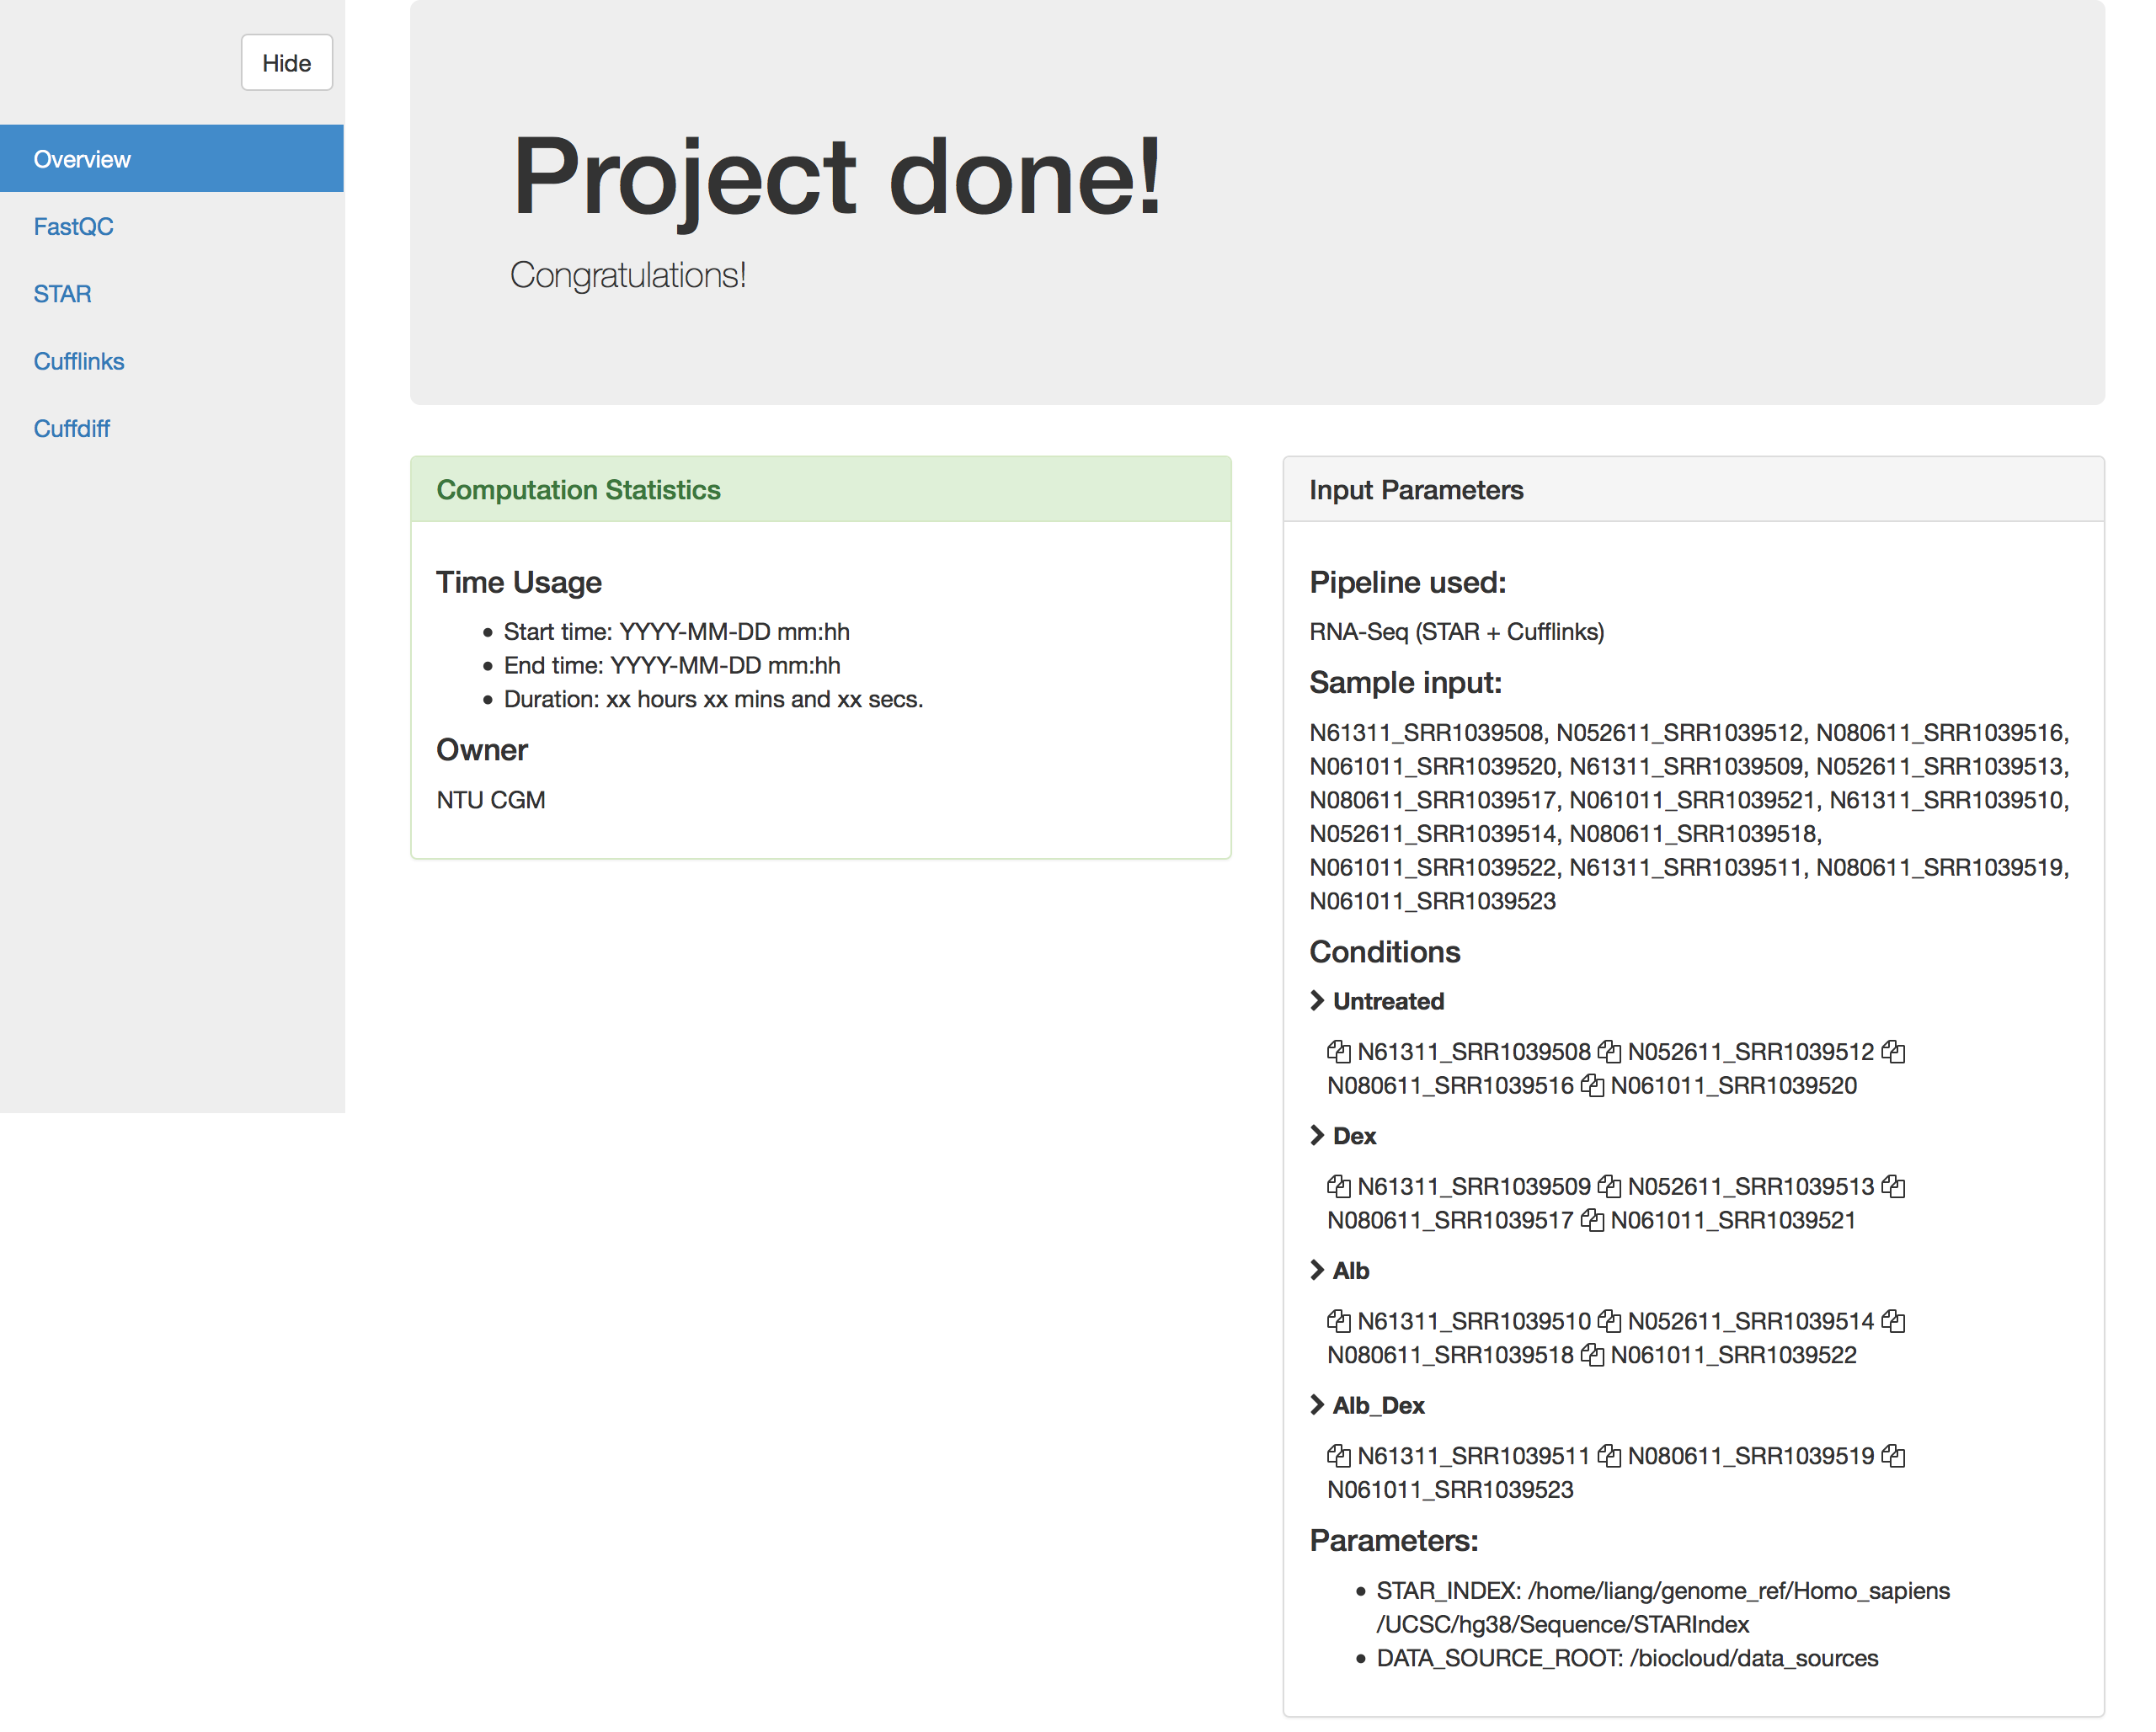
\includegraphics[width=1\textwidth]{images/report_home}
\caption[Result summary report]{
    Result summary report.
}
\label{fig:report}
\end{figure}



\begin{figure}[!tb]
\centering
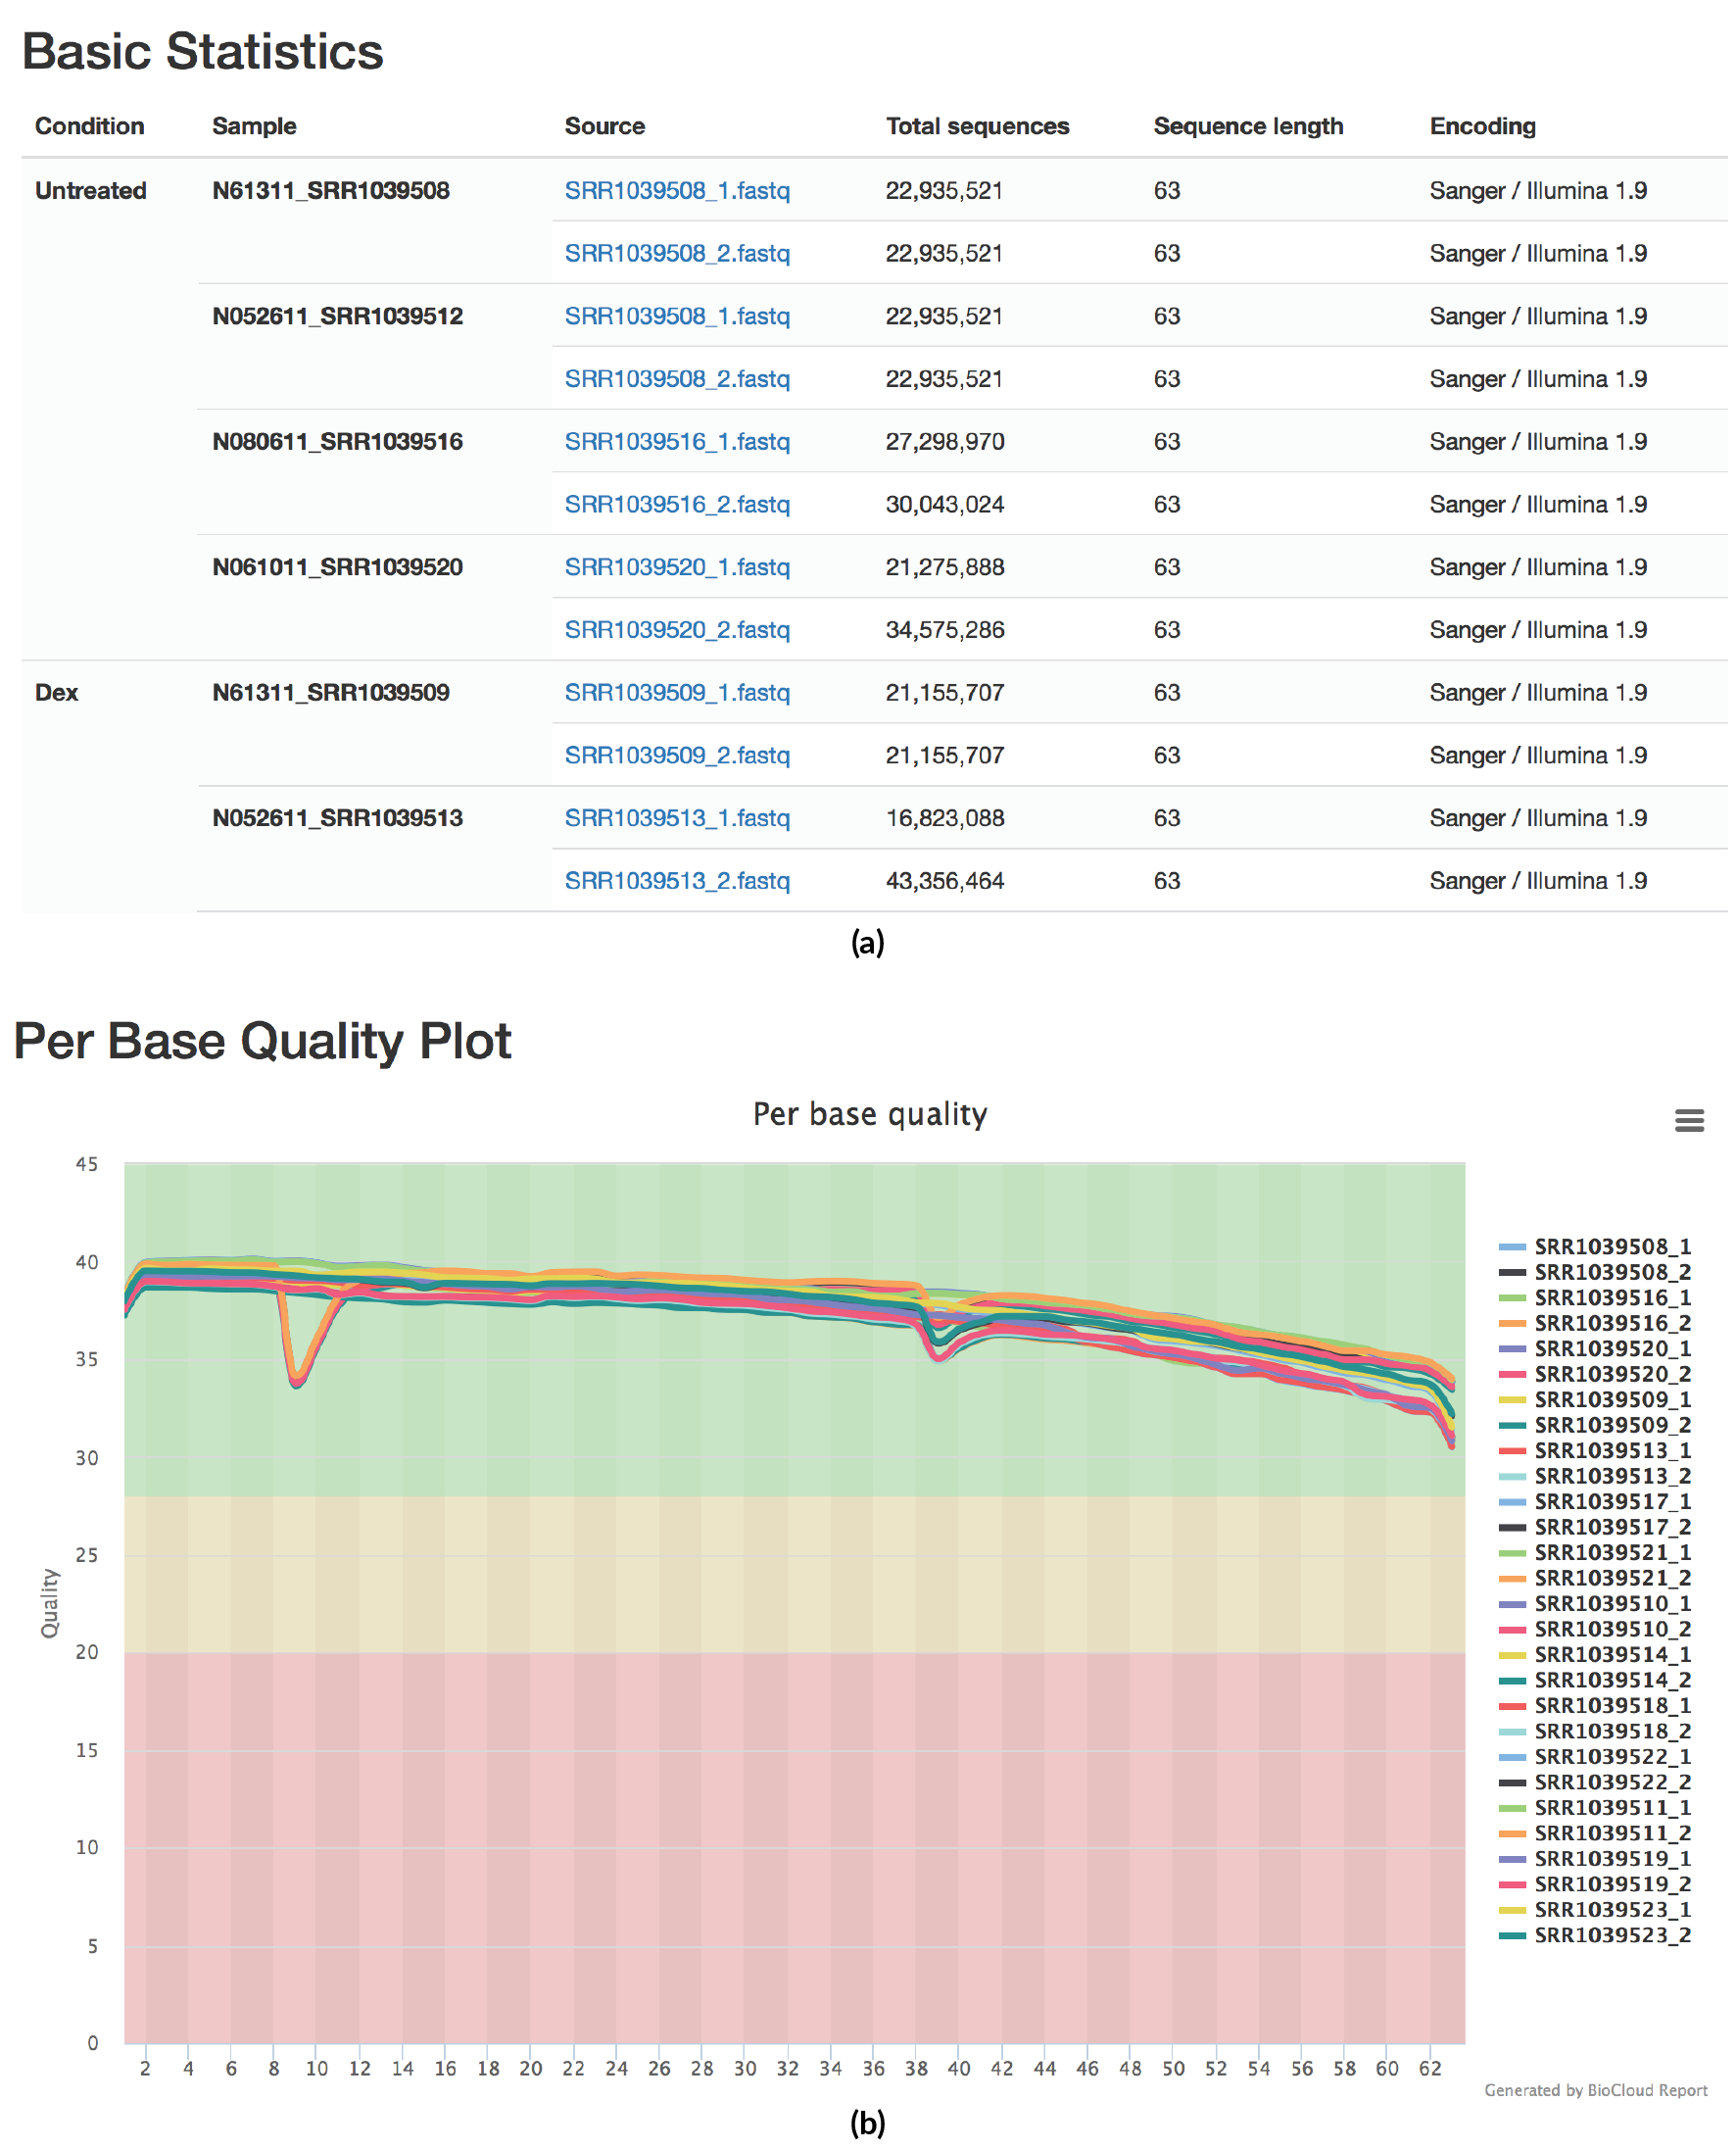
\includegraphics[width=1\textwidth]{images/report_qc}
\caption[Quality check page of report]{
    Quality check page of report.
}
\label{fig:report-qc}
\end{figure}


Raw output by each tools were provided via separate download links in the last
section of each report page. These raw output links can be further integrated
with popular genome browsers like Ensembl\footnote{
    Current Ensembl v84 release does not support HTTPS connections to remote
    BAM files due to an older version of samtools was used. However, in the
    next release the HTTPS connection will be supported and all operations on
    UCSC genome browser can be applied to Ensembl genome browser in a similar
    fashion.
} and UCSC genome browser. Here we take the alignment BAM files from breast cancer
dataset and display the alignment on UCSC genome browser as example, shown in
Figure~\ref{fig:result-genome-browser}. User specified custom data track by the
following format:

\begin{CVerbatim}[fontsize=\small]
track type=bam name="NBS1"
bigDataUrl=https://biocloud.cgm.ntu.edu.tw/access/<auth key>/result/
STAR/NBS1/Aligned.sortedByCoord.out.bam
\end{CVerbatim}

\vspace{-1em}\noindent
Here the data track was specified for NBS1 sample from the breast cancer
dataset. User can then view their alignment on UCSC genome browser in the same
way as on desktop genome browser tools like IGV. Genome browser didn't download
the whole BAM file before displaying the alignment. Instead, it utilized the
BAM index to look up the alignment data of the current viewing genomic region.
Many file formats other than BAM are supported, including GTF and VCF.

\begin{figure}[!p]
    \centering
    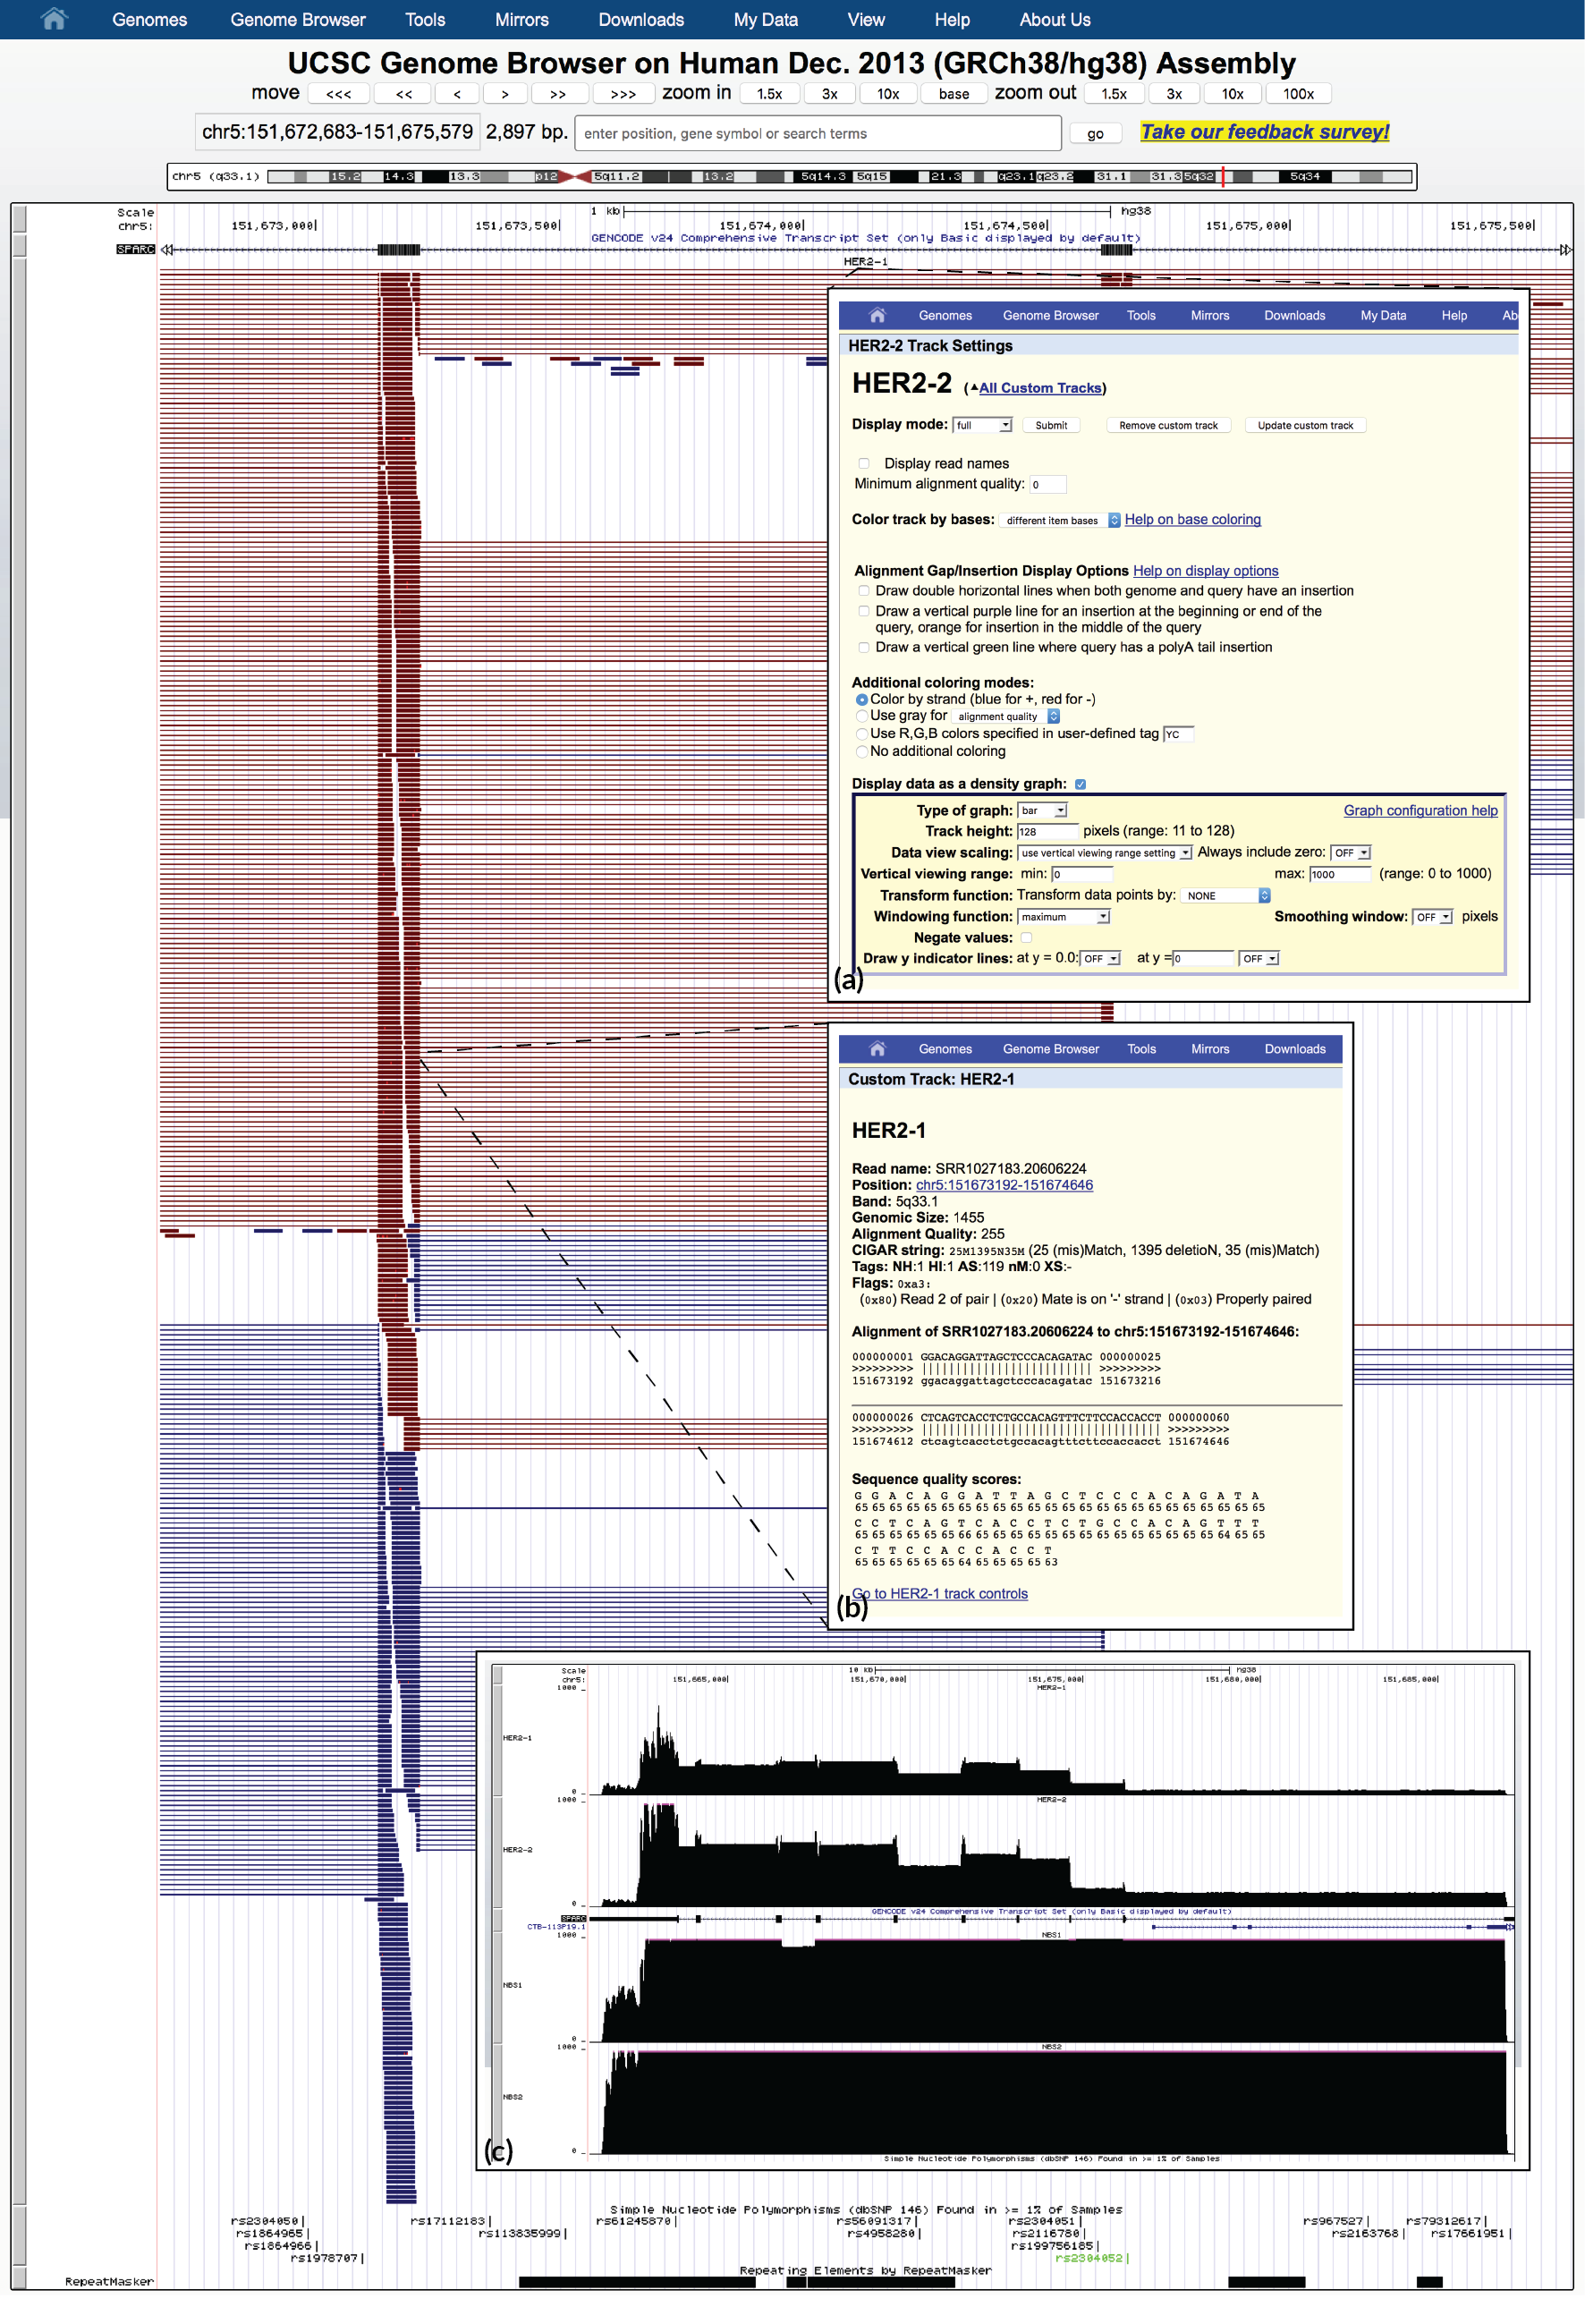
\includegraphics[width=1\textwidth]{images/result_genome_browser}
    \caption[Result integration with genome browser]{
        Result integration with USCS genome browser. Alignment of HER2-1 sample
        was shown. Display options can be tuned in the panel shown in (a). By
        clicking on an read, detail alignment information poped up as shown in
        (b). In (c), genome browser was configured to display the coverage
        depth of four samples simultaneously.
    }
    \label{fig:result-genome-browser}
\end{figure}




% \subsection{Alignment - STAR}
% \subsection{Cufflinks}
% \subsection{DESeq2}

% vim: set textwidth=79 spell:

\chapter{Discussions}
\label{c:discussion}


\section{Data source upload}

BioCloud does not offer the ability to upload data sources from local to
BioCloud's data storage since the uploading is extremely hard to implement
correctly and few people use uploading function anyway. Uploading a pair-end
sample of 22M 63 base pair long reads takes about 3.5 hours for normal ADSL
connection or 20 minutes for education network to complete\footnote{The upload
speed is given 1MB/s for normal ADSL connection and 10MB/s for education
environment; The pair-end sample of 22M reads with 63 base pair consumes total
12 GiB disk space}. Upload a dataset having 10 samples may take days for users
of low connection speed. Though a lot of HTTP-based uploading frameworks exist,
they are only suitable for uploading few hundreds of MBs at a time. Moreover,
most users may not upload any data sources in their lifetime since their raw
sequencing data exist on the server in the very first place. BioCloud supports
reading soft-linked data sources so putting data sources under BioCloud data
storage structure does not necessarily increase the total disk usage. When data
source transferring is needed, one can use tools such as \texttt{rsync},
\texttt{sftp} and \texttt{ftp} to help transfer large files rather than using
HTTP-based solutions. After data sources appear in the user's data source
directory, they can be discovered and managed by BioCloud.



\section{Pipeline extension}
\label{s:pipeline-extension}

% \begin{lstlisting}
% class Hello:
%
%     def __init__(self, a, b):
%         self.x = a
%         self.y = b
%
%     @classmethod
%     def from_str(cls, raw_str):
%         return cls(*raw_str.split('\t', 1))
% \end{lstlisting}


\section{Collaboration with other frameworks}

% vim: set textwidth=79:

\chapter{Conclusions}
\label{c:conclusion}


\@startappendix

% \chapter{Datasets}
\label{c:dataset}


\backmatter

\clearpages
\phantomsection
\addcontentsline{toc}{chapter}{\bibname}

% Your bibliography goes here
\printbibliography

\end{document}
